% for details https://github.com/alwynmathew/phd-thesis-cseiitp
%% PLEASE READ THE COMMENTS BEFORE DOING ANYTHING 
\documentclass[12pt,letter]{book} % Font size=12, tamaño hoja carta, both-side printing, and in a book format
\usepackage[spanish]{babel}
\usepackage[utf8]{inputenc}
\usepackage[intlimits]{amsmath}%
\usepackage{booktabs}
\usepackage{adjustbox}
\usepackage{longtable}
\usepackage{multicol}
\usepackage{lscape}
\usepackage{amsthm}
\usepackage{caption3}
\usepackage{graphicx}
\usepackage{latexsym}
\usepackage{thesis}
\usepackage{rotating}
\usepackage{wrapfig}  % for biography photo
% \usepackage{pstricks} % for table shading https://tex.stackexchange.com/a/68871/136315
\usepackage{colortab} % for table shading
%\usepackage[algoruled, algochapter, linesnumbered]{algorithm2e} % for algorithm writing
%\usepackage{indentfirst}  % for indent the first paragraph of any chapter
\usepackage{makeidx}      % for making index at last in the thesis
\makeindex                % for making index at last in the thesis
\allowdisplaybreaks[1]
\usepackage{gensymb}
\usepackage{amssymb}

\usepackage{tabularx}
\usepackage{blindtext}
\usepackage{amstext}
\usepackage{epstopdf}
\usepackage{dcolumn}
\usepackage{array,multirow}
\usepackage{tikz}
\usepackage{titlesec}
\titlespacing*{\subsection}
{0pt}{0.6\baselineskip}{0.6\baselineskip}
\titlespacing*{\section}
{0pt}{0.75\baselineskip}{0.75\baselineskip}
\titlespacing*{\subsubsection}
{0pt}{0.5\baselineskip}{0.5\baselineskip}

%\newtheorem{theorem}{Theorem}
%\newtheorem{condition}{Condition}

%#### sectstyCAMBIA EL FORMATO DEL CAPTITULO
\usepackage{sectsty}

%\chapterfont{\centering}
%\chaptertitlefont{\centering}
\usepackage{titlesec}
%####################################
%\titleformat{\chapter}[display]
%  {\normalfont\bfseries\LARGE}
%  {\chaptertitlename~\thechapter}{0.5pc}
%  {{\color{black}\titlerule[1pt]\vspace{0.1pc}\titlerule[3.5pt]}\vspace{1pc}}%\MakeUppercase}
%####################################
%\renewcommand{\thechapter}{\Roman{chapter}}}
%\titleformat{\chapter}[display]
%{\bfseries\LARGE}
%{\MakeUppercase{\chaptertitlename} \Huge\thechapter}{0ex}
%{%\titlerule
%	\vspace{0.5ex}%
%	}
%	[\vspace{1ex}%
%	\titlerule]
%####################################
%\titleformat{name=\chapter,numberless}[display]
%	{\normalfont\bfseries\LARGE}{}{1pc}
%	%{\MakeUppercase{\chaptertitlename} \Huge\thechapter}{1ex}
%	{\MakeUppercase{\chaptertitlename}}
%####################################
%\titleformat{name=\chapter,numberless}[display]
%  {\normalfont\bfseries\LARGE}{}{1pc}
%  {\MakeUppercase}

%####################################
%\usepackage{caption}
%\usepackage{subcaption}
  
% Uncomment the following block and comment the next block (both starting with '\usepackage[dvips...') when you need for final printout. However to submit the softcopy of the thesis comment the first block and uncomment the next block.

%%-------------------- 1st Block ----------------------------
%\usepackage[dvips,
%                 bookmarks,
%                 bookmarksopen=true,
%                 bookmarksnumbered=true,
%                 breaklinks=true,
%                 linktocpage,
%                 backref,
%                 colorlinks=true,
%                 linkcolor=black,
%                 urlcolor=black,
%                 citecolor=black,
%                 anchorcolor=black,
%                 hyperindex=true,
%                 hyperfigures
%                 ]{hyperref} % added by Sandipan
%
%\usepackage{backrefx}% added by Sandipan
%-------------------- 1st Block Ends-------------------------

%-------------------- 2nd Block -----------------------------
%\usepackage[dvips]{hyperref} % for link boxes
%\usepackage[dvipdfmx]{hyperref} % for dvi to pdf conversion
%\usepackage[driverfallback=dvipdfm]{hyperref}
\usepackage[pdftex]{hyperref}
\hypersetup{
             bookmarks,
             bookmarksopen=true,
             bookmarksnumbered=true,
             breaklinks=true,
             linktocpage,
             backref,
             colorlinks=true, % false: boxed links; true: colored links
             linkcolor=cyan,    % color of internal links
             filecolor=magenta,
             citecolor=red,  % color of links to bibliography
             urlcolor=cyan,    % color of external links
             hyperindex=true,
             anchorcolor=blue,
             hyperfigures
}

%\usepackage{backrefx} % for citing the section/page_no of each reference in Bibliography
%\usepackage[all]{hypcap} % for showing the figure as well as its caption.

%%--------------------2nd Block Ends--------------------------

\setcaptionwidth{0.9\textwidth} % For caption width 'Caution: Don't Change otherwise you'll be in trouble to control the figure/Table captions.
%\usepackage[linewidth=1pt]{mdframed}
\usepackage{minibox}
%\usepackage{algorithm}
\usepackage{algpseudocode}
\usepackage{enumitem}

\usepackage{arydshln}
\usepackage{multirow}
\usepackage{calc}
\usepackage{verbatim}
\usepackage{bbding}
\usepackage{bbm}
\usepackage{soul}
\usepackage{dsfont}
\usepackage{mathrsfs}
\usepackage{mathtools}

\usepackage[caption=false]{subfig}
%\usepackage[ruled]{algorithm2e}
\usepackage{algorithm} 
%\usepackage{algorithmic}  
%\usepackage[algo2e]{algorithm2e}
%\usepackage[latin1]{inputenc}
%\newtheorem{theorem}{Theorem}
\newcommand{\cmt}[1]{ }
\usepackage{lipsum}

\newcommand{\thesistitle}{Propuesta de modelo para pronóstico del precio de Bitcoin y su clasificación para la toma de decisiones de inversión}
\newcommand{\authorname}{Sacbe García García}
%\newcommand{\authorrollno}{XX21CSXX}
\newcommand{\supervisorname}{Dr. Álvaro Castañeda Mendoza\\ \vspace{0.2cm}Mtr. Carlos Abraham Carballo Monsivais}

\begin{document}

% ------------ Starting of Preamble Pages---------------------
%\pagenumbering{none}
%%\pagestyle{empty} %%%%%%%%%%%%%%%%%%%%%%%%%%%%%%%%%%%%%%%%%%%%%%%%
\thispagestyle{plain}
\begin{center}
\vspace*{0.5cm}
{\Large \bf MOMENT METHOD ANALYSIS OF RECTANGULAR WAVEGUIDE DISCONTINUITIES USING HIGHER-ORDER HIERARCHICAL LEGENDRE BASES\\}
\end{center}



\vspace{14cm}
\begin{flushright}
%\begin{Large}
\begin{large}
{\bf {\em Yatendra Kumar Singh ~~}\noindent}
%\vskip -.8\baselineskip
%\noindent
%\rule[-2.5 mm]{\textwidth}{3 pt}\\}
%\end{Large}
\end{large}
\end{flushright}

%\cleardoublepage

\setcounter{page}{1}
\pagenumbering{roman}
	
%\thispagestyle{plain}
\thispagestyle{empty}
\vspace*{0.50cm}
\begin{center}
	\begin{figure}[t]
		\centering
		
\includegraphics[width=0.3\textwidth]{HeadTail/unistmo.jpeg}
	\end{figure}
 {\LARGE  {\thesistitle}\\}

\vspace*{1.20cm}
{ Presentado en cumplimiento parcial de los requisitos
\\
para el grado de
}\\

\vspace*{1.0cm}
{\Large {Licenciado en Matemáticas Aplicadas}}\\

\vspace*{0.5cm}
{por}\\

\vspace*{0.5cm}
{\Large{\authorname}}\\
%{ \authorrollno}\\

\vspace*{1cm}
{ Bajo la supervición de:}\\

\vspace*{0.3cm}
{\large{ \supervisorname}}\\

\vspace*{0.50cm}

%\begin{figure}[h]
%\centering
%  
\includegraphics[width=3.5cm,height=3.5cm]{HeadTail/iitplogo.eps}
%\end{figure}

\vspace*{0.50cm}
%{ Department of Computer Science and Engineering\\
%Indian Institute of Technology Patna \\
%Bihar, India - 801106 \\
%April ~\the\year}\\
{ Matemáticas Aplicadas\\
Universidad del Istmo campus Tehuantepec\\
Oaxaca, México - 70760\\
\today} \\%~\the\year}\\
\vspace{1.8cm}

%Copyright
%\copyright~\the\year ~\authorname.  All rights reserved.
\end{center}

\clearpage

\thispagestyle{plain}
\clearpage

\cleardoublepage

% \thispagestyle{empty}%
% \vspace*{0.4\textheight}
% \begin{center}
% {\AlgoFont{18} {\sf To Him}}\\
% \vspace*{0.5\baselineskip}
% {\AlgoFont{18} {\sf The Source of Everything}}\\
% \end{center}

\cleardoublepage

%\addcontentsline{toc}{chapter}{Certificate of Approval} 
%\cmt{
\vspace*{0.5cm}
\begin{minipage}[b]{0.3\textwidth}
		
\includegraphics[width=2.5cm, height=2.5cm]{HeadTail/iitplogo.eps}
\end{minipage} 
\begin{minipage}[b]{0.7\textwidth}
	\flushleft
\textbf{INDIAN INSTITUTE OF TECHNOLOGY PATNA}\\
\textbf{Department of Computer Science \& Engineering}
\end{minipage}
\noindent\rule{16cm}{1pt}
}
\vskip 2.0\baselineskip
\centerline{\textbf{APPROVAL OF THE DOCTORAL COMMITTEE}}
\noindent\rule{16cm}{1pt}
\vskip 2.0\baselineskip

%\begin{flushright}
%    30/06/2010
%\end{flushright}


\noindent
Certified that the thesis entitled \textbf{\textquotedblleft \thesistitle\textquotedblright} submitted by \textbf{\authorname} to Indian Institute of Technology Patna for the award of the degree of Doctor of Philosophy, has been accepted by the doctoral committee members after the successful completion of the synopsis seminar held on 22 July 2019.

% \noindent
% Certified that the synopsis entitled \textbf{\textquotedblleft \thesistitle\textquotedblright} submitted by \textbf{Rakesh Kumar Sanodiya} to Indian Institute of Technology Patna for the award of the degree of Doctor of Philosophy, has been accepted by the doctoral committee members after the successful completion of the synopsis seminar held on 22 July 2019.

\vspace*{2.5cm}

\begin{table}[h]
\begin{tabular}{lp{2.1 cm}l}
\textbf{Dr. W}  						&   &  	\textbf{\supervisorname}  \\
Chairperson, Doctoral Committee  		&   &  	Supervisor \\
Department of Computer Sc. and Engg. 	&  	& 	Department of Computer Sc. and Engg.\\
Indian Institute of Technology Patna 	&   & 	Indian Institute of Technology Patna \\

\vspace*{1.5cm}\\

\textbf{Dr. Y} 							&  & \textbf{Dr. Z}    \\
Member, Doctoral Committee     			&  & Member, Doctoral Committee         \\
Department of Computer Sc. and Engg. 	&  & Department of Electrical Engineering   \\
Indian Institute of Technology Patna 	&  & Indian Institute of Technology Patna  \\
\end{tabular}
\end{table}

\vspace*{1.5cm} 

% \begin{table}[h] 
% \begin{tabular}{lp{0.5 cm}l}
% \textbf{Dr. Sudhan Majhi} & &   \\
% Member, Doctoral Committee & &      \\
% Department of Electrical Engg. & &  \\
% Indian Institute of Technology Patna & &     \\
% \end{tabular}
% \end{table}


 
% After the viva-voce, change the file name to 'Certificate_of_approval.tex'
%\cleardoublepage

%\addcontentsline{toc}{chapter}{Declaration}
%\cmt{
\vspace*{1cm}
\begin{minipage}[b]{0.3\textwidth}
	
\includegraphics[width=2.5cm, height=2.5cm]{HeadTail/iitplogo.eps}
\end{minipage} 
\begin{minipage}[b]{0.7\textwidth}
	\flushleft
	\textbf{INDIAN INSTITUTE OF TECHNOLOGY PATNA}\\
	\textbf{Department of Computer Science \& Engineering}
\end{minipage}
}

\vskip 2.0\baselineskip
\centerline{\textbf{DECLARATION BY THE SCHOLAR}}
\noindent\rule{16cm}{1pt}
\vskip 2.0\baselineskip


\noindent
I certify that:

\begin{itemize}
	\item The work contained in this thesis is original and has been done by me under the guidance of my supervisor.
	\item  The work has not been submitted to any other Institute for any degree or diploma.
	\item I have followed the guidelines provided by the Institute in preparing the thesis.
	\item I have conformed to the norms and guidelines given in the Ethical Code of Conduct of the Institute.
	\item Whenever I have used materials (data, theory and text) from other sources, I have given due credit to them by citing them in the text of the thesis and giving their details in the reference section.
	\item The thesis has been checked by anti-plagiarism software.
\end{itemize}


\vspace*{2.5cm}
\begin{flushright}
\authorname
\end{flushright}

%\cleardoublepage

%\addcontentsline{toc}{chapter}{Certificate}
%\cmt{
\vspace*{0.5cm}
\begin{minipage}[b]{0.3\textwidth}
	
\includegraphics[width=2.5cm, height=2.5cm]{HeadTail/iitplogo.eps}
\end{minipage} 
\begin{minipage}[b]{0.7\textwidth}
	\flushleft
	\textbf{INDIAN INSTITUTE OF TECHNOLOGY PATNA}\\
	\textbf{Department of Computer Science \& Engineering}
\end{minipage}
}

\vskip 2.0\baselineskip
\centerline{\textbf{\large{CERTIFICATE}}}
\noindent\rule{16cm}{1pt}
\vskip 2.0\baselineskip

%\vskip 2.0\baselineskip
%%\centerline{\underline{\Large{\bf Certificate}}}
%\centerline{\textbf{\Large{CERTIFICATE}}}
%\vskip 2.0\baselineskip
\noindent
This is to certify that the thesis entitled \textbf{\textquotedblleft \thesistitle \textquotedblright}, submitted by \textbf{\authorname} to Indian Institute of Technology Patna, is a record of bonafide research work under my supervision and I consider it worthy of consideration for the degree of Doctor of Philosophy of the Institute.


\vspace*{1.5cm}


\begin{table}[h]
\begin{tabular}{lp{1.1 cm}l}
  &   &  \textbf{\supervisorname}  \\
  &   &  Supervisor \\
Place: Indian Institute of Technology Patna  &  & Department of Computer Sc. and Engg.\\
Date: \today  &   & Indian Institute of Technology Patna \\
\end{tabular}
\end{table}
%\cleardoublepage

\addcontentsline{toc}{chapter}{Agradecimientos}
\chapter*{Agradecimientos}
%I would like to express my deep and heartfelt gratitude for my respected guide and mentor, Dr. -, for his evergreen blessings, valuable advice, support, good wishes and encouragement all alone the journey of this work. Without his undisputed support, this work would not have been true in the light of daylight. I am also grateful to the members of my Doctoral Committee (Dr.  -, Dr.  -, and Dr. -) for reviewing my works and for their valuable comments.

\lipsum[66]

\vspace*{1.5cm}
\begin{flushright}
\authorname
\end{flushright}


\vspace*{-1.3cm}
\noindent
Lugar: Universidad del Istmo\\
Fecha: \today 

\cleardoublepage

\addcontentsline{toc}{chapter}{Resumen}
\chapter*{Resumen}

El bitcoin es una criptomoneda que ha adquirido una gran popularidad y su precio se ha incrementado enormemente, sin embargo, posee una gran volatilidad y se vuelve necesario predecir su comportamiento. En el presente trabajo, a partir de las características de la blockchain descargadas desde el 2 de febrero de 2012 al 14 de abril de 2022 usando la API de coinmetrics se analizaron aquellas que tuvieran un mayor impacto en el precio del bitcoin usando análisis de regresión, PCA y un dendrograma de correlación.

Con las características obtenidas de la blockchain y con datos del precio del bitcoin calculados a partir de la mediana de tres fuentes distintas (Yahoo Finance, Investing y Coingecko) con un intervalo igual al de las métricas de la blockchain se muestran los resultados de aplicar métodos estadísticos como Naive, SES, Holt, ETS, ARIMA y métodos de aprendizaje máquina como RTS, SVM, RF y LSTM, para predecir el precio del bitcoin con el objetivo de realizar una comparación entre métodos con base en el índice de error RMSE y el índice de eficiencia Theil’s U. Los datos del precio son transformados por funciones log, BoxCox, diff y diff(log) como también la escala original y se mostrará una tabla comparativa con los índices de error y exactitud por transformación para elegir el modelo propuesto.

De igual forma se estudia la geometría de los datos usando análisis topológico de datos para deducir que a partir de la norma $C^1$ generada del diagrama de persistencia, se pueden anticipar caídas graves del precio y crear alertas de cracs financieros.

Por último, con ayuda de la característica topológica y el cálculo de la entropía de Shannon del precio del bitcoin se obtienen clusters de inversión para el etiquetado de imágenes, estas últimas elaboradas a partir de la serie de tiempo financiera, que son clasificadas para la toma de decisiones de inversión utilizando CNN. El modelo generado es empleado para dar una recomendación de compra, venta o riesgo y mejorar futuros modelos de inversión a mediano y largo plazo.

Se concluye que hay métricas que influyen en la varianza del precio y que además mejoran los modelos de predicción, por otra parte, el análisis topológico de datos ayuda a detectar exitosamente caídas del precio, asimismo también ayuda a la creación de clusters de inversión junto con la entropía de Shannon para la mejora de toma de decisiones de inversión.


\cleardoublepage

%%%%%%%%%%%%%%%% LIST OF ABBREVIATIONS %%%%%%%%%%%%%%%%%%
%	\addcontentsline{toc}{chapter}{List of Abbreviations}
%	\markboth{List of Abbreviations}{List of Abbreviations}
%	% Give Abbreviations alphabetically
\chapter*{Abreviaturas}\label{LstAbb} 

\begin{flushleft}
\begin{longtable}{lp{11cm}}

OHLC & Open-High-Low-Close\\
SLR & Systematic Literature Review\\	
AI & Artificial Intelligence \\
DL & Deep Learning \\
SES & Simple Exponential Smoothing\\
ETS & Exponential Smoothing\\
ARIMA & Autoregressive Integrated Moving Average\\
RTS & Regression Time Series\\
SVM & Support Vector Machine\\
RF & Random Forest\\
LSTM & Long Short Term Memory\\

\end{longtable}
\end{flushleft}

%	\clearpage{\pagestyle{empty}\cleardoublepage}

%%%%%%%%%%%%%%%%%% LIST OF SYMBOLS %%%%%%%%%%%%%%%%%%%%%
%    \addcontentsline{toc}{chapter}{List of Symbols}
%	\markboth{List of Symbols}{List of Symbols}
%	% Greek Symbols are to be given first followed by other symbols alphabatically
\chapter*{Lista de Notaciones y Operaciones}\label{LstSym}

\begin{flushleft}
\begin{longtable}{lp{12cm}}
	
$X$ & Unknown 1\\
$\mathcal{K}_0$ & Unknown 2\\


\end{longtable}
\end{flushleft}


%	\clearpage{\pagestyle{empty}\cleardoublepage}

%%%%%%%%%%%%%%%%%%%%%%%%%%%%%%%%%%%%%%%%%%

\addcontentsline{toc}{chapter}{Abstract}
\chapter*{Abstract}

\lipsum


\vspace*{0.7cm}
%\vspace*{1cm}
\noindent
{\large{\textbf{\emph{Keywords:}}}}~
Keywords 1, Keywords 2, Keywords 3








	
%\addcontentsline{toc}{chapter}{List of Publications}
%\chapter*{Contribuciones}
\addcontentsline{toc}{chapter}{Contribuciones}
%\section*{Publicaciones}
%
%\begin{enumerate}
%	
%	\item One
%	\item Two	\textit{(Under revision)}
%	\item Three \textit{(Under review)}
%
%\end{enumerate}

\section*{Congresos}


\begin{enumerate}

	\item \textbf{Sesión de cartel}: "Bitcoin: Prónostico y clasificación para toma de decisiones de inversión'' G. Sacbe y A. Castañeda, en 4 Congreso Nacional de la Sociedad Matemática Mexicana ''Intégrate para derivar soluciones'' llevado a cabo el Del 18 al 22 de octubre 2021 en la sala virtual de la Escuela de Desarrollo de Habilidades Científicas y de Innovación.
	\item \textbf{Conferencia}: ''Análisis de métricas de la blockchain con mayor influencia en el precio del bitcoin y clasificación de la criptomoneda para toma de decisiones de inversión usando CNN'' G. Sacbe y Carballo Carlos en el Centro de Investigación en Matemáticas, durante la Escuela de Verano virtual en los meses de junio y agosto de 2021.
	\item \textbf{Sesión de cartel}: "Propuesta de Modelo de Machine Learning para pronósticos de la Criptomoneda Bitcoin'' G. Sacbe y Carballo Carlos durante la XIX Escuela de Probabilidad y Estadística en Guanajuato, Gto., México, el 23 de Abril de 2021.

\end{enumerate}

\section*{Otros}

\begin{enumerate}
	\item \textbf{Hackaton:} ''Mejorando la Toma de Decisiones para Inversionistas'' Equipo Bitmoney conformado por Ballesteros Leticia, Carballo Carlos, García Sacbe en Decred TalentLand Latinoamerica llevado a cabo durante del 17 de noviembre al 2 de diciembre de 2020.
\end{enumerate}



\noindent
\rule{0.49\textwidth}{0.75pt} $_{\bigcirc}$ \rule{0.49\textwidth}{0.75pt}\\









\renewcommand{\headrulewidth}{0.30pt}    % Width of head rule

%%%%%%%%%%%%%%%%%% LIST OF SYMBOLS %%%%%%%%%%%%%%%%%%%%%
%\addcontentsline{toc}{chapter}{List of Tables}
%\listoftables
%\cleardoublepage

%\clearpage{\pagestyle{empty}\cleardoublepage}
%\addcontentsline{toc}{chapter}{List of Figures}
%\listoffigures
%\cleardoublepage

%\clearpage{\pagestyle{empty}\cleardoublepage}
%\addcontentsline{toc}{chapter}{Lista de Simbolos}
%\markboth{List of Symbols}{List of Symbols}
%% Greek Symbols are to be given first followed by other symbols alphabatically
\chapter*{Lista de Notaciones y Operaciones}\label{LstSym}

\begin{flushleft}
\begin{longtable}{lp{12cm}}
	
$X$ & Unknown 1\\
$\mathcal{K}_0$ & Unknown 2\\


\end{longtable}
\end{flushleft}



\clearpage{\pagestyle{empty}\cleardoublepage}
\addcontentsline{toc}{chapter}{Lista de Abreviaturas}
\markboth{List of Abbreviations}{List of Abbreviations}
% Give Abbreviations alphabetically
\chapter*{Abreviaturas}\label{LstAbb} 

\begin{flushleft}
\begin{longtable}{lp{11cm}}

OHLC & Open-High-Low-Close\\
SLR & Systematic Literature Review\\	
AI & Artificial Intelligence \\
DL & Deep Learning \\
SES & Simple Exponential Smoothing\\
ETS & Exponential Smoothing\\
ARIMA & Autoregressive Integrated Moving Average\\
RTS & Regression Time Series\\
SVM & Support Vector Machine\\
RF & Random Forest\\
LSTM & Long Short Term Memory\\

\end{longtable}
\end{flushleft}

\clearpage{\pagestyle{empty}\cleardoublepage}

%%%%%%%%%%%%%%%%%%%%%%%%%%%%%%%%%%%%%%%%%%

\tableofcontents
\cleardoublepage

%%%------------- End of the Preamble Pages----------------------------

%%%------------- Starting of the Actual Thesis -----------------------
    \renewcommand{\headrulewidth}{0.30pt} 
	\setcounter{page}{1}
	\pagenumbering{arabic}

\begin{spacing}{1.4}

\chapter[Introducción]{Introducción}{Introducción}\label{Intro}
%\vspace{2cm}
\noindent
\rule{0.49\textwidth}{0.75pt} $_{\bigcirc}$ \rule{0.49\textwidth}{0.75pt}\\

El mercado de las criptomonedas se ha disparado en los últimos años y a comparación  de las monedas tradicionales las mayores innovaciones de los activos criptográficos son establecer un nuevo sistema de pago con sistemas criptográficos sofisticados, transacciones de persona a persona, con un sistema descentralizado y que asegura la privacidad del usuario.\\
El Bitcoin destaca exitosamente en todos los puntos anteriores consolidándose como la criptodivisa líder del mercado.
Debido a su naturaleza altamente volátil se necesitan buenas predicciones en las que basar las decisiones de inversión. En los mercados financieros tradicionales puede interesar la aplicación de estrategias comerciales automatizadas que ayudan a obtener un rendimiento razonable de los fondos invertidos.\\

\noindent
\rule{0.49\textwidth}{0.75pt} $_{\bigcirc}$ \rule{0.49\textwidth}{0.75pt}\\
\clearpage

\section{Introducción}
%\begin{figure}[h]
%	\centering
%	\includegraphics[width=0.5\textwidth]{example-image-a}
%	\caption{Test Figure}
%	\label{fig1: intro}
%\end{figure}
Bitcoin es la primera implementación de un concepto conocido como moneda criptográfica, la cual fue descrita por primera vez en 1998 por Wei Dai. La especificación inicial del protocolo Bitcoin y la prueba del concepto la publicó Satoshi Nakamoto en el 2009  la cual abandonó a finales de 2010 sin revelar nada de su persona, desde entonces la comunidad ha crecido de forma exponencial \parencite{nakamotoBitcoinPeertoPeerElectronic2008}.

En noviembre de 2020 el bitcoin alcanzó máximos históricos \parencite{BitcoinUSDBTCUSD} consolidándose así como una moneda legitima que desde finales de 2019 se ha disparado más del $175\%$, incluso gigantes de pago como Paypal y Square permiten la compra y venta de bitcoins. Países como Estados Unidos, Japón y El Salvador actualmente permiten transacciones con esta moneda, destacando este último por ser el primer país en legalizar el bitcoin como moneda legal a partir del 7 de septiembre de 2021. En contraste, países como La República Dominicana o China no cuentan con el respaldo de sus bancos centrales, inclusive prohibiendo éste último la compra y venta de esta criptomoneda.

La tecnología Bitcoin es popular ya que permite evitar pasar por un intermediario para validar una transacción, genera valor al realizar las validaciones, y este valor se transforma en un elemento de intercambio. Como se ha visto en los últimos años el bitcoin puede recuperar su valor después de caídas significativas, incluso cuando la incertidumbre es alta en el mercado como durante la pandemia de la COVID-19 \parencite{mudassirTimeseriesForecastingBitcoin2020}, esto es importante ya que consolida a esta moneda como un activo de inversión fiable.
%Pero, ¿cómo funciona esta moneda?%

%El funcionamiento de esta moneda es como sigue, se define una moneda electrónica como una cadena de firmas digitales donde cada propietario al transferir una monto a otra persona, éste firma digitalmente un \textit{hash} de la transacción previa y la clave pública del siguiente propietario, añadiendo ambos al final de la moneda [4]. Este conjunto de transacciones es público y propagada a todos los usuarios en la red, esto también es conocido como blockchain o cadena de bloques, donde cada bloque es una transacción con los hashes correspondientes, eliminando así la centralización y la confianza en un solo punto.%

Se define una moneda electrónica como una cadena de firmas digitales donde cada propietario, al transferir un monto a otra persona, firma digitalmente un \textit{hash} de la transacción previa y la clave pública del siguiente propietario, añadiendo ambos al final de la moneda \parencite{nakamotoBitcoinPeertoPeerElectronic2008}. Este conjunto de transacciones es público y propagado a todos los usuarios en la red. Esto también es conocido como blockchain o cadena de bloques, donde cada bloque contiene una transacción con los hashes correspondientes, eliminando así la centralización y la confianza en un solo punto.

%Aquí un hash es una función matemática que genera una cadena de caracteres $M$ que resume un mensaje $U$ a través de una función computable (Ver apéndice A).%
%Entonces, ¿cómo podemos asegurar que alguien no puede inventarse una transacción?%

Se puede asegurar que alguien no puede agregar una transacción maliciosa en la blockchain ya que se utiliza una prueba de trabajo o proof of work. Para llevar a cabo esta prueba primero se tiene que convertir un bloque de la cadena de bloques en un hash y ser verificado, esto es, comprobar que el hash cumpla con un número de ceros requeridos en un orden especifico o dicho de otra, forma resolver un problema criptográfico que requiere poder computacional. Al agregarse otro bloque el atacante tiene que asegurarse que este esté conectado a su bloque malicioso por lo que tiene que competir contra el poder computacional de los demás usuarios de la red y así indefinidamente, lo que resulta inviable. La red blockchain selecciona la cadena de bloques más larga, esto quiere decir que selecciona la cadena de bloques que resuelve los problemas criptográficos más rápido, siendo la más confiable por ser la soportada por la comunidad.

Por todo lo anterior y debido a su naturaleza altamente volátil, se necesitan buenas predicciones en las que basar las decisiones de inversión. En los mercados financieros tradicionales puede interesar la aplicación de estrategias comerciales automatizadas que ayudan a obtener un rendimiento razonable de los fondos invertidos. Los métodos tradicionales (Naive, SES, Holt, ETS y ARIMA) dependen en gran medida de una hipótesis que requiere datos con estacionalidad, tendencia y ruido para que sean eficaces. Al no cumplirse estas características los mecanismos de inteligencia artificial entran en acción, considerando especialmente la naturaleza volátil y temporal de los datos como los del bitcoin \parencite{tandonBitcoinPriceForecasting2019}.

\section{Motivación}
En la literatura disponible se muestran resultados limitados sobre aplicaciones y desarrollo de métodos con el uso de aprendizaje automático y trasfondo matemático para la toma de decisiones de inversión en criptomonedas \parencite{felizardoComparativeStudyBitcoin2019,tandonBitcoinPriceForecasting2019,phaladisailoedMachineLearningModels2018}. Este campo tiene dos oportunidades de desarrollo potencial: la primera aplicando los métodos existentes en la creación de parámetros de comparación y su capacidad para caracterizar el entorno real, la segunda buscar alternativas de modelación para fines de predicción.
Esta propuesta de investigación permitirá contribuir al cuerpo de conocimiento de la ciencia de datos con nuevos métodos para la caracterización de oportunidades de inversión financiera. Se espera que al final de la investigación se proponga al menos un método eficiente y robusto para facilitar a consultores de inversiones, analistas de riesgos e incluso inversionistas no calificados en la mejora de toma de decisiones para crecer sus inversiones a mediano y largo plazo.

\section{Planteamiento del problema}
Actualmente los métodos y herramientas para realizar modelación y caracterización de tendencias de comportamiento financiero están limitados al uso de técnicas simples en la mayoría de los casos prácticos \parencite{zbikowskiApplicationMachineLearning2016}. El problema a resolver es encontrar un modelo de predicción para el precio del bitcoin en dólares usando las métricas de la blockchain que más influyen en su comportamiento utilizando reducción de dimensionalidad y análisis topológico de datos, como también, proponer un modelo que ayude a la toma de decisiones de inversión.

\section{Objetivo}
\subsection{Objetivo general}
Proponer un modelo de aprendizaje máquina para predecir el precio del bitcoin usando métricas financieras y de la blockchain, averiguar si estas influyen en su volatilidad y %cómo también%
plantear una metodología para la clasificación de estos precios para toma de decisiones de inversión a mediano y largo plazo.

\subsection{Objetivos específicos}
Los objetivos de la investigación son:
\begin{itemize}
	\item Identificar si hay métricas que influyen en la variabilidad del precio del bitcoin y si es el caso, determinar las de mayor peso usando análisis de regresión, análisis de componentes principales y agrupamiento jerárquico.
	\item Aplicar modelos estadísticos y de aprendizaje máquina sobre datos transformados para predecir el precio del bitcoin.
	\item Seleccionar el mejor modelo con base al índice de error RMSE y el índice de eficiencia Theil's U.
	\item Describir el panorama persistente de los datos usando análisis topológico de datos.
	\item Caracterizar diferentes herramientas de inteligencia artificial que permitan mejorar la toma de decisiones en un mercado financiero.
	\item Clasificar la decisión de inversión a mediano y largo plazo en comprar, vender o arriesgar.
\end{itemize}

\section{Contribuciones}
Se espera que la contribución de esta investigación sea un modelo que minimice el error mínimo cuadrático en las predicciones y que estas sean fiables conforme al índice Theil's U, esto se reflejará en que los pronósticos realizados no diferirán mucho con respecto al precio original.
Por otro lado se pretende aportar una metodología que ayude a clasificar el precio predicho para toma de decisiones de inversión
a mediano y largo plazo a diferencia de los modelos para trading actuales.
\vspace{-0.5cm}
\section{Alcances y limitaciones}
La investigación del estado de arte se limita a las publicaciones de herramientas y algoritmos que se han publicado recientemente. La comparación sera exclusiva entre los métodos de predicción y clasificación seleccionados en la investigación (Naive, SES, Holt, ETS, ARIMA, RTS, SVM, RF, LSTM y CNN). Se usan datos experimentales (series de tiempo del precio del bitcoin) para estimar la eficiencia y robustez de los métodos, los resultados tienen validez en el mismo contexto de los datos experimentales y las limitaciones de los métodos.
\vspace{-0.5cm}
\section{Contenido general}
A continuación se mostrará de manera breve y concreta lo que el lector encontrará en cada capítulo.

\begin{enumerate}
	\item \textbf{Introducción}: Presentación breve sobre orígenes del bitcoin, objetivos, justificación y contribuciones de la investigación.
	
	\item \textbf{Estado del arte}: Aquí se hace referencia a la revisión sistemática de la literatura y se encuentra una revisión en la cual se presentan de forma cronológica los avances de los distintos tópicos mostrados en la introducción. 
	
	\item \textbf{Metodología propuesta}: Se explica tomando como punto de partida un diagrama de flujo que muestra todo el proceso de la tesis y luego se explica a detalle el uso de cada método y herramienta usada.
	
	\item \textbf{Fundamento teórico}: Se detalla el trasfondo matemático de cada medida, modelo, transformación y análisis utilizado.
	
	\item \textbf{Resultados en Bitcoin}: Este capítulo describe los resultados obtenidos siguiendo la metodología propuesta.
	
	\item \textbf{Conclusiones y trabajo futuro}: Conclusiones generales.
\end{enumerate}


 
\chapter[Estado del arte]{Estado del arte}{Estado del arte}\label{Intro}
\renewcommand{\tablename}{Tabla}

\noindent
\rule{0.49\textwidth}{0.75pt} $_{\bigcirc}$ \rule{0.49\textwidth}{0.75pt}\\

Los modelos de inteligencia artificial ya sean de aprendizaje maquina o aprendizaje profundo han mostrado ser los mejores para predecir el precio volátil de algunas criptomonedas, entre ellas el bitcoin. Esto se debe a que los datos del precio no cumplen con los supuestos de estacionalidad, tendencia y ruido de algunos modelos estadísticos requieren.\\
Otros estudios muestran la importancia de agregar métricas tecnológicas como la de la blockchain como variables explicativas para mejorar la predicción utilizando métodos basados en correlación o análisis de sensibilidad.\\
Se encuentra también que los modelos de clasificación más comunes para inversión en criptomonedas están basados en el trading, donde la clasificación toma en cuenta las alzas o bajas del precio con respecto al actual en intervalos pequeños de tiempo, y con una exactitud un poco mayor al del tiro de una moneda.\\

\noindent
\rule{0.49\textwidth}{0.75pt} $_{\bigcirc}$ \rule{0.49\textwidth}{0.75pt}\\
\clearpage

\section{Metodología} 

Para el seguimiento del estado del arte se utilizó la revisión sistemática de la literatura (SLR) expuesta en el \autoref{appen3} donde se detalla cada paso de la misma. Esta metodología consiste en interpretar y sintetizar de forma adecuada la información obtenida de un tema de investigación. Se deben cumplir tres fases principales en una SLR: (1) Planificación de revisión, (2) Realización de la revisión, (3) Reporte de resultados. Los resultados para cada apartado de la investigación realizada se muestran a continuación utilizando los estudios principales obtenidos en la SLR de forma cronológica.

\section{Predicción del precio}

En un artículo publicado en marzo del 2018 McNally et al. \cite{mcnallyPredictingPriceBitcoin2018} compararon modelos que utilizan redes neuronales recurrentes (RNN), modelos long-short term memory (LSTM) y ARIMA para realizar una clasificación binaria que determine las subidas y bajadas del precio con respecto al valor anterior. Para la clasificación se evaluó el rendimiento de la regresión utilizada para predicción con el indicador de error RMSE.
En este trabajo se mostró que el modelo LSTM genera una mejor exactitud para la clasificación, sin embargo, basados en el RMSE el mejor modelo fue RNN con datos que van desde el 19 de agosto de 2013 a 19 de julio de 2016. 

%con un RMSE tan bajo cómo 6.87\% 

En julio de 2018 Phaladisailoed et al. \cite{phaladisailoedMachineLearningModels2018} publicaron un articulo utilizando datos de Bitstamp que abarcan desde el 1 de enero de 2012 hasta 8 de enero de 2018 en intervalos de un minuto para realizar trading con Bitcoin. Se utilizaron todas características financieras del formato OHLC y se alcanzó un mejor rendimiento con el modelo GRU (Gated Recurrent Unit) entre LSMT, Theil-Sen Regression y Huber Regression. 

%con un error cuadrático medio (MSE) de 0.00002 y un $R^2$ de 99.2\%.

Por otro lado en el artículo publicado en marzo de 2019 Tandon et al. \cite{tandonBitcoinPriceForecasting2019}, utilizando datos de CoinMarket sobre modelos como RNN, LSTM, regresión lineal y random forest (RF) con 10-fold cross validation, se mostró que RNN con LSTM supera a random forest y regresión lineal usando como predictores el precio de cierre y volumen del mismo con datos desde 2013 a 2019.

%alcanzando un error medio absoluto (MAE) de 0.0043 con 10-fold cross validation usando RNN con LSTM, superando a random forest y regresión lineal usando como predictores el precio de cierre y volumen del mismo con datos desde 2013 a 2019.

En un estudio comparativo de octubre de 2019 realizado por Felizardo et al. \cite{felizardoComparativeStudyBitcoin2019} nos muestran los resultados de modelos como ARIMA, RF, SVM, LSTM y Wavenets concluyendo que el modelo SVM es el mejor a un día de predicción y a una ventana de cinco a diez días SVM y ARIMA son superiores a los demás modelos con datos de 2012 hasta inicios del 2017.

%Concluyó que el modelo SVM es el mejor a un día de predicción con un MAE de  11.41 y un MSE de 376.615, a cinco y diez días. SVM y ARIMA son superiores con entre 22.494 y 36-26 de MAE y un rango de 1076.32 a 2188.53 de MSE respectivamente con datos de 2012 hasta inicios del 2017.


En julio de 2020 Mudassir et al. \cite{mudassirTimeseriesForecastingBitcoin2020} obtienen resultados utilizando características de la blockchain, para ello se redujo la dimensionalidad de los datos filtrando las características con análisis de componentes principales y random forest, del análisis se seleccionaron aquellas características con mayor importancia, resultando que la arquitectura LSTM fue la mejor entre los modelos ANN, SVM y SANN.

%En predicción la arquitectura LSTM fue la mejor con un MAE de 22.05, RMSE de 36.12 y MAPE de 3.83 con un horizonte de 7 días.

De los estudios disponibles se concluye que no hay una metodología establecida para la predicción del precio del bitcoin, ya sea por las fechas de los datos de entrenamiento, los indices de comparación o los horizontes de predicción, esto puede deberse a que el Bitcoin es una tecnología en desarrollo y que los distintos modelos requieren de supuestos estadísticos distintos. 
Por otra parte, de los modelos utilizados más populares, el LSTM es que el que más destaca ya que fue el mejor en dos de cinco artículos primarios.


%De los estudios disponibles se concluye que no hay medidas de comparación estándar para la predicción, esto es debido a los diferentes modelos usados y que para su comparación todos deben tener un indice de comparación definido.
%Por otra parte, de los modelos utilizados más populares, el LSTM es que el que más destaca alcanzando como mínimo un error medio absoluto de 0.0043 con validación cruzada en el trabajo de Tandon et al. \cite{tandonBitcoinPriceForecasting2019} de 2019.

\section{Análisis de métricas} 

En abril de 2018 tenemos un articulo de Saad et al. \cite{saadCharacterizingBlockchainbasedCryptocurrencies2018} sobre la caracterización de la blockchain donde se trata de identificar las métricas que explican los altos precios alcanzados. Usando la correlación de Pearson entre criptomonedas y características de la blockchain se encontró que el número de carteras, hashrate y UTXO determinan el número de nuevos usuarios, mineros y el balance que pueden gastar todos estos. 

%Usando regresión lineal sobre estas características se encontró que con datos de abril de 2016 a septiembre de 2017 se obtuvo un RMSE sobre el precio de 0.0113 y un MAE de 0.0060 haciendo predicción sobre los cuatro meses próximos.

En septiembre de 2019 Ji et al.  \cite{jiComparativeStudyBitcoin2019} encontraron que usando la correlación de Spearman con veintinueve características de la blockchain dieciocho de ellas fueron seleccionadas incluyendo el precio. De la selección se excluyeron aquellas características que tuviesen un coeficiente de Spearman menor a 0.75 y mayores a 0.95, esto debido a que las características con un coeficiente cercano a uno eran propiedades que dependían explícitamente del precio como la capitalización del mercado. De las características seleccionadas las que obtuvieron un mayor coeficiente fueron difficulty, est-trans-vol-usd, hash-rate, my-wallets, trade-vol y trans-fees-usd.

En julio de 2020 Mudassir et al. \cite{mudassirTimeseriesForecastingBitcoin2020} obtienen características de la blockchain filtrando estas con análisis de componentes principales y random forest, seleccionando aquellas con mayor importancia. En el estudio no se muestran las características obtenidas por el PCA pero este logra capturar un 95\% de la varianza de los datos, sin embargo, el rendimiento en los modelos de regresión con estas características fue menor de lo esperado.
Se utilizó random forest como método principal de selección de características donde la importancia de las mismas dependía de la ventana de tiempo utilizada para el análisis. Las características más importantes que se mantuvieron a lo largo de las distintas ventanas de tiempo fueron las siguientes: median\_transaction\_fee30trxUSD, size90trx, price3wmaUSD, difficulty30rsi, mining\_profitability y transactionvalueUSD. 

%Con estas métricas de la blockchain la predicción con la arquitectura LSTM fue la mejor con un MAE de 22.05, RMSE de 36.12 y MAPE de 3.83 con un horizonte de 7 días.

En enero de 2021 Chen et al. \cite{chenMachineLearningModel2021} partiendo de predictores económicos y tecnológicos, y seleccionando aquellas con un factor de importancia utilizando random forest y ANNs se encontró que entre los modelos propuestos (ARIMA, SVR, ANFIS y LSTM) LSTM fue el mejor usando como datos de entrada los predictores obtenidos con el análisis de factor de importancia. Se encontró también que los predictores tecnológicos de alto impacto cambian constantemente con respecto al tiempo. En adición se muestra que la tarifa promedio por transacción es un fuerte predictor con alta importancia. Se concluye que las características que se mantienen en el tiempo (del 1 de enero de 2011 a 31 de julio de 2018) con alto impacto son la capitalización del mercado y la tarifa promedio por transacción.

%El modelo LSTM alcanzó como mínimo un RMSE promedio de 12.0632, un MAPE de 2.2793, y un MAE de 8.7512 usando estos predictores en cuatro ventanas de tiempo diferentes.

Con esto, el estudio concluyó que la información obtenida de determinantes económicos y tecnológicos son más importantes que únicamente la tasa de cambio de la moneda (precio en USD) aun en periodos largos de tiempo como los usados en el estudio (1 de julio de 2015 a 31 de julio de 2018). 

El panorama del estado del arte en lo que respecta al análisis de métricas de la blockchain para mejorar la predicción del precio parece no muy concluyente. En la mayoría de los estudios primarios se realiza un análisis de correlación, ya sea usando correlación de Pearson o de Spearman, estas nos indican el grado de relación lineal que hay entre las variables. Chen y Mudassir et al. \cite{chenMachineLearningModel2021, mudassirTimeseriesForecastingBitcoin2020} utilizan el método de análisis de sensibilidad para medir la importancia de los factores económicos y tecnológicos usando random forest y artificial neural networks. Los resultados generales de los estudios no nos muestran características en común concluyentes. Eliminando las variables como la capitalización del mercado que son dependientes directamente del precio tenemos que la tarifa promedio por transacción, el hashrate, y el número de carteras son algunas características en común en al menos dos de los estudios.



\section{Clasificación del precio para inversión}
 
 
En febrero de 2020 Chen et al. \cite{chenBitcoinPricePrediction2020} usando clasificación binaria, características de la blockchain y financieras clasificaron los precios del bitcoin con modelos estadísticos como regresión lineal y análisis lineal de discriminante en intervalos de 5 minutos alcanzando una exactitud del 53\%. Por otro lado métodos de machine learning como random forest, XGBosst, discriminante cuadrático, SVM, y LSTM alcanzaron en promedio una exactitud del 62.2\%.
La clasificación considero las subidas y bajadas del precio con respecto al actual y las características de la blockchain para predicción fueron seleccionadas usando Boruta. 

%%\begin{itemize}
%%	\item Block size
%%	\item Hash rate
%%	\item Mining difficulty
%%	\item Time between blocks
%%	\item Trades per minute
%%	\item Number of transaction
%%	\item Confirmed transactions per day
%%	\item Mempool transaction count
%%	\item Market capitalization
%%	\item Estimated transaction value
%%	\item Total transaction value
%%	\item Mempool size
%%\end{itemize}

En mayo de 2020 Pintelas et al. \cite{pintelasInvestigatingProblemCryptocurrency2020} mostraron que la combinación de algoritmos de deep learning (LSTM, Bi-directional LSTM, Convolutional Layers) con estrategias de ensamble (everaging, baggin, stacking) se pueden complementar mostrando buena auto-correlación en los residuos.  En Bitcoin se alcanzó una exactiud de 54.62\% con el modelo CNN-BiLSTM y ensamble Bagging. La clasificación tomó en cuenta la dirección del precio con respecto al actual.

En julio de 2020 Mudassir et al. \cite{mudassirTimeseriesForecastingBitcoin2020} obtuvieron resultados utilizando características de la blockchain, filtrando estas con análisis de componentes principales o random forest y seleccionando aquellas con mayor importancia. En la clasificación se alcanzó un promedio por arriba de un 65\% de exactitud para el día siguiente. Para 7 y 9 días se obtuvo de un 62\% a 64\% de exatitud con los modelos propuestos ANN,SVM,SANN y LSTM. 

En Septiembre de 2020 Jaquart et al. \cite{jaquartShorttermBitcoinMarket2021} realizaron clasificación con datos de movimiento a corto plazo (1-60 minutos). El conjunto de características usadas incluyen características técnicas (retorno del bitcoin), de la blockchain (número de bitcoins, transacciones), de sentimiento (Sentimiento de Twitter y Sentimiento de Twitter ponderado por la fuerza de la emoción), y características base del activo (S\&P500, VIX returns, Gold returns, MSCI World returns). Se usaron los modelos GRU, LSTM, FNN (Feedforward neural networks), regresión logística, gradiend boosting clasifier y random forest. Se concluyó que aparentemente incrementar el intervalo de tiempo trading aumentaba la exactitud del mismo. Se obtuvo el mejor resultado con LSTM a 60 minutos de predicción (56\%) con datos de 4 de marzo de 2019 a 10 diciembre de 2019.

En enero de 2021 Ibrahim et al. \cite{ibrahimPredictingMarketMovement2021} realizaron clasificación del precio haciendo predicción hacia arriba o hacia abajo en intervalos de tiempo de 5 minutos. Se comparan modelos como ARIMA, Prophet (Facebook), RF, RF lagged-Auto-regression y multi-layer perceptron. El estudio concluyó que MLP alcanzó la mejor exacitud con 54\%.

En febrero de 2021 Akyildirim et al. \cite{akyildirimPredictionCryptocurrencyReturns2021} realizaron clasificación de precios del bitcoin para trading de un día, 15, 30, 60 min. utilizando el criterio -1 si OPEN$<$CLOSE y 1 si OPEN$>$CLOSE refiriéndose a el precio de apertura y cierre en un periodo de tiempo abarca desde 10 agosto de 2017 a 23 junio de 2018. Se alcanzó una exactitud de 55-65\% en promedio resultando ser SVM el mejor modelo entre regresión logística, ANN y random forest como modelos candidatos.

En general podemos observar que los métodos de clasificación se basan en el trading y la dirección del precio, esto es, se utilizan datos de movimiento a corto plazo para realizar una predicción de compra o venta. Los resultados obtenidos en el estado del arte  tienen una exactitud un poco mayor al del tiro de una moneda, sin embargo la metodología propuesta por Mudassir \cite{mudassirTimeseriesForecastingBitcoin2020} alcanza una exactitud máxima de 64\% con ventana de tiempo de 7 a 9 días, haciendo notar que tal vez el trading no sea la mejor estrategia de inversión, sino las inversiones a mediano y largo plazo.
 % new chapters 
\chapter[Metodología]{Metodología propuesta}{Metodología Propuesta}\label{Metodologia}

\noindent
\rule{0.49\textwidth}{0.75pt} $_{\bigcirc}$ \rule{0.49\textwidth}{0.75pt}\\

La metodología se basa en la recolección de datos, el pre-procesamiento de los mismos, en fases de entrenamiento para los distintos modelos usados y su respectiva validación con sus indicadores de error y eficiencia.\\
Para mejorar la calidad de la toma de decisiones de inversión se agregó un análisis de métricas antes de la fase de entrenamiento para saber cuales son las características de la blockchain que más variabilidad agregan al precio. Por ultimo se hizo una inspección a los datos usando análisis topológico para poder predecir posibles tiempos de crisis.\\
La salida de esta metodología es un posible precio en un intervalo de tiempo futuro, una recomendación de inversión y una posible advertencia de una crash en la serie de tiempo financiera.\\
%Al final de este flujo de trabajo se toma una decisión para invertir 

\noindent
\rule{0.49\textwidth}{0.75pt} $_{\bigcirc}$ \rule{0.49\textwidth}{0.75pt}\\
\clearpage

\section{Metodología}

La metodología propuesta se divide en cuatro apartados: La predicción del precio utilizando series de tiempo del bitcoin en dólares, el análisis de las métricas de la blockchain, la clasificación de las alzas y bajas del precio y el análisis topológico de datos.
 
En la predicción del precio se darán a conocer rendimientos futuros utilizando un conjunto de datos de prueba sobre el cual se realizará la predicción usando modelos estadísticos y de machine learning. Para el análisis de métricas de la blockchain se encontrarán las variables que más influyen en el precio del bitcoin utilizando análisis de regresión, análisis de componentes principales y clustering jerárquico, por otra parte la clasificación para toma de decisiones de inversión a mediano y largo plazo convertirá la serie de tiempo en imágenes y las clasificará en comprar, vender o incertidumbre utilizando redes neuronales convolucionales, por último, el análisis topológico de datos analizará posibles crashes en el precio utilizando la norma topológica C1 y k-means.

La metodología general del trabajo se muestra en la \autoref{fig4}. Esta se divide en el pre-procesamiento de los datos, la fase de entrenamiento, análisis de métricas, análisis topológico de datos y la fase de validación. 

\subsection{Datos y pre-procesamiento}

Los datos del precio del bitcoin están disponibles en linea de forma gratuita. Los datos para este estudio fueron recolectados de tres fuentes distintas, Yahoo! Finance \cite{YahooFinanceStock}, Kraken \cite{BitcoinCryptocurrencyExchange} e Investing \cite{InvestingComStock}, para la descarga de estos datos se usó la librería \emph{quandl} en Python para descargarlos de forma automática en formato OHLC (Open-High-Low-Close). El intervalo de los datos es considerado desde el 2 de febrero del 2012 hasta el 11 de octubre de 2021.

Las tres fuentes de datos mostraban diferencias al compararlas, no todas estaban en formato OHLC y habían gaps entre los precios. Para solucionar lo anterior se creó la función \emph{merge\_dfs\_on\_column} en Python, que tiene por entrada una lista de dataframes con columnas en común, una lista con los nombres de exchanges usados asociados a los dataframes y la columna en común sobre la cual se trabajará. Esta función devuelve un dataframe que combina las columnas en común especificadas. Las columnas de dataframe obtenido anteriormente son sumadas y dividas entre el número de columnas, creándose así una única columna con la media.
%A las columnas del dataframe obtenido se le calculan la media creándose una única columna.
%\newpage
\begin{landscape}
	\begin{figure}[h]
		\centering
		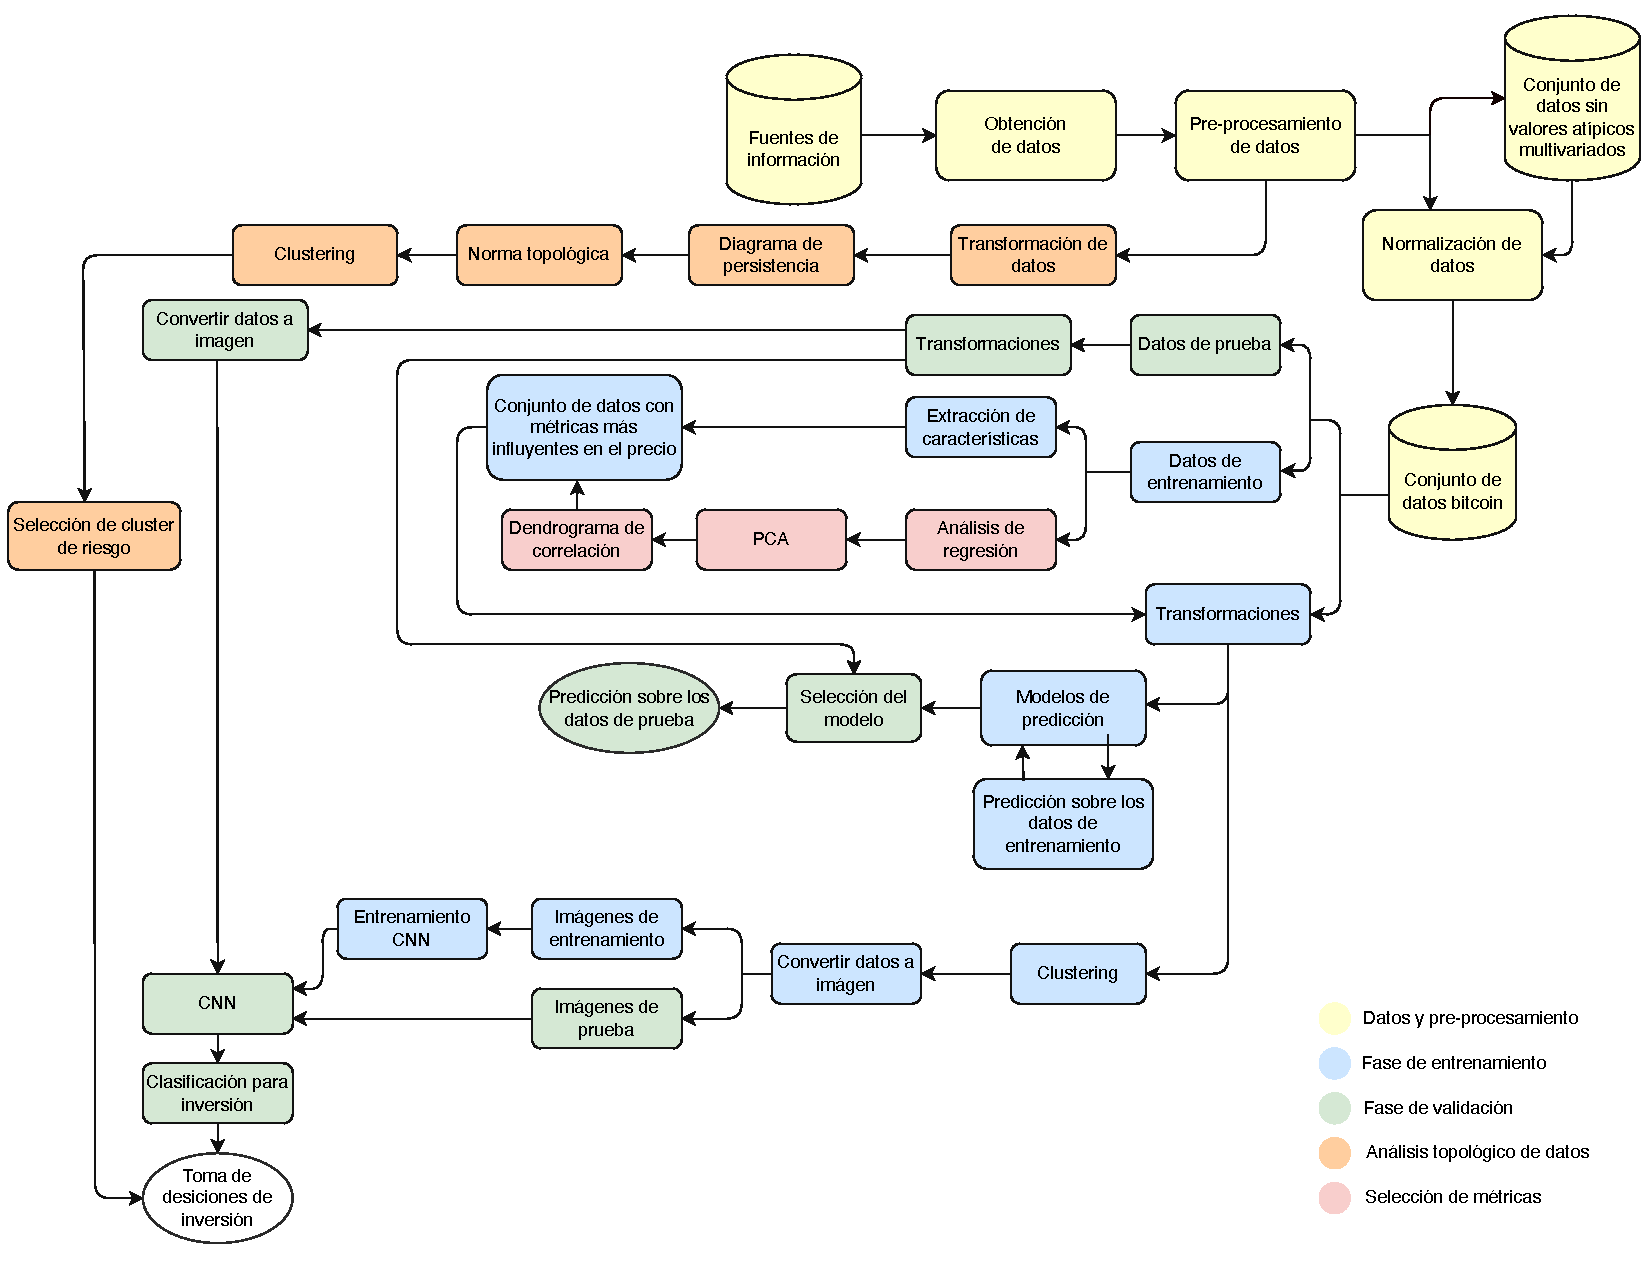
\includegraphics[scale=0.7]{Chapter3/Meto-2.pdf}
		\caption{Metodología general propuesta}
		\label{fig4}
	\end{figure}
\end{landscape}
%\clearpage
Al final se crea un conjunto de datos usando como columnas las medias obtenidas utilizando la función antes especificada. Ya que algunos exchanges no registran los precios con precisión o no trabajan en días festivos o fines de semana, entonces se eliminan estas fechas al dataframe creado con la media de los precios y se inputan los datos faltantes utilizando interpolación splines cúbico en ambas direcciones.\\
Los datos para realizar el análisis de métricas fueron recolectados utilizando la API de la comunidad de Coin Metrics \cite{APIBasics}. Se obtuvo un archivo CSV con un total de 140 métricas como se observa en la \autoref{tab:TableAppen1}. Se consideró un intervalo de los datos desde el 2 de febrero del 2012 hasta el 11 de agosto de 2021 donde se utilizó interpolación de splines de orden tres para igualmente inputar datos faltantes.

Se eliminaron los valores atípicos multivariados del conjunto de datos de métricas utilizando la distancia de  Mahalanovis definida como sigue:

\[ D_M(x) = \sqrt{(x-\mu)\textbf{S}^{-1}(x-\mu)} \]

donde $x = (x_1,x_2,x_3,...,x_N)^T$ es una observación, $\mu = (\mu_1,\mu_2,\mu_3,...,\mu_N)^T$ es la media y $\textbf{S}$ es la matriz de covarianza. Se considera un valor atípico si la distancia del dato (la métrica en este caso) encontrada es mayor que dos veces la media de las distancias.


Se escalaron los datos de las métricas como del precio al intervalo [0,1] con la formula $(x-min(x))/(max(x)-min(x))$ del método MinMax para un mejor funcionamiento de los algoritmos de machine learning. 	 

\subsection{Fase de entrenamiento}

Las bases de datos creadas se dividieron con un 80\% para los datos de entrenamiento y 20\% para los datos de prueba. Para los datos de predicción el conjunto de entrenamiento contiene 2782 elementos. Para el conjunto de entrenamiento de métricas de la blockchain se utilizó la función \emph{train\_test\_split} de la librería sklearn en Python creando de forma aleatoria 3604 datos con semilla 123. Por último, después de las transformaciones correspondientes el conjunto de entrenamiento para clasificación y toma de decisiones de inversión resulto en 616 imágenes.

\subparagraph{Predicción del precio:} Para la extracción de características de los modelos de machine learning se usó el método de correlación \cite{tandonBitcoinPriceForecasting2019}, donde se realizó la estimación del coeficiente de correlación de Pearson para examinar la fuerza y la dirección de la relación lineal entre las variables de la base de datos, en este caso, apertura, precio máximo, mínimo y cierre. Se determinó que todas las características están fuertemente relacionadas entre sí y fueron utilizadas como variables explicativas en los modelos no univariados (SVM, RF, RTS). A las características extraídas se les agregó las métricas de la blockchain que más influyeron en la variabilidad del precio como se detalla en la \autoref{ssec:metrics}.    
Para las redes LSTM se utilizó únicamente el precio de cierre con retraso de un día para su ajuste.

Antes de aplicar los modelos a los datos de entrenamiento se realizaron distintas transformaciones como BoxCox [\ref{eqn:9}], $\log$ [\ref{eqn:10}], $diff$ [\ref{eqn:11}] y $diff$($\log$) [\ref{eqn:12}]. Para la transformación BoxCox el parámetro $\lambda$ se estimó con la función BoxCox.lambda() de R para encontrar el parámetro que mejor estabiliza la varianza, en el caso del la transformación $\log$ se uso la base natural $e$.

Se ajustaron los precios del bitcoin usando diferentes modelos estadísticos y de machine learning basados en el método Naive [\ref{eqn:1}], SES [\ref{eqn:2}], Holt [\ref{eqn:3}], ETS \footnotemark , ARIMA [\ref{eqn:4}], RTS [\ref{eqn:5}], SVM [\ref{eqn:6}], RF [\ref{eqn:7}], y LSTM [\ref{eqn:8}].

Para el método Naive, SES, Holt, ETS y ARIMA se usaron las funciones estándar de R del paquete \emph{fpp2}, únicamente cambiando la entrada de los datos de entrenamiento por la respectiva transformación, por otro lado, para el método RTS, SVM y RF se realizaron las inferencias sobre las características dichas anteriormente, manteniendo los hiperparámetros por defecto. La configuración usada para el modelos LSTM es la mostrada en la \autoref{tab:Table10}.

%Tabla hiperparámetros LSTM
\begin{table}[!h]
	\centering
	\begin{tabular}{p{4cm} p{4cm}  }
		\toprule
		\textbf{Hiperparámetro} & \textbf{Configuración}\\
		\midrule
		Optimizer & Adam\\
		Hidden layers & 2 (2,1)\\
		Learning rate & 0.02\\
		Epochs & 100\\
		Batch size & 1\\
		Activation & tanh\\
		Loss function & MSE\\
		\bottomrule
		\hline
	\end{tabular}
	\caption{Configuración de los hiperparámetros LSTM}
	\label{tab:Table10}
\end{table}

%Tabla transformaciones
\begin{table}[h]
	\centering
	\begin{tabular}{m{4cm} m{8cm}}
		\toprule
		\textbf{Transformación} & \textbf{\hspace{4cm}Fórmula}\\
		\midrule
		BoxCox			& 
		
		\begin{equation}
			\label{eqn:9}
			y_{t}(\lambda)= \left\{ \begin{array}{lcc}
				
				\frac{y_{t}^{\lambda} - 1}{\lambda} &   si  & \lambda \neq 0 \\
				\log{y_{y}} &  si & \lambda = 0 \\
				
			\end{array}
			\right.
		\end{equation}  
		\\ 
		log			&
		\begin{equation}
			\label{eqn:10}
			y_{t} = \log{y_{t}}
		\end{equation} \\
		\emph{diff} 			&
		\begin{equation}
			\label{eqn:11}
			\nabla y_{t} = y_{t} - y_{t-1}
		\end{equation}
		\\
		\emph{diff}(log)		& 
		\begin{equation}
			\label{eqn:12}
			\nabla y_{t} = \log{y_{t}} - \log{y_{t-1}}
		\end{equation}\\
		\bottomrule
		\hline
	\end{tabular}
	\caption{Transformaciones utilizadas en el modelo de entrenamiento}
	\label{tab:Table9}
\end{table}

\footnotetext[1]{Encuentra el modelo que minimiza mejor el AIC (Akaike’s Information Criterion) o BIC (Schwarz’s Bayesian Information Criterion) usando SES de primer, segundo o tercer orden.}

%Tabla modelos utilizados
\begin{table*}
	\centering
	\begin{adjustbox}{width=0.95\textwidth}
	\begin{tabular} {m{2cm} m{9cm} m{7cm}}
		\toprule
		\textbf{Modelo} & \textbf{\hspace{3cm}Notación} & \textbf{Parámetros}\\
		\midrule
		Naive&\begin{equation}\label{eqn:1}\hat{y}_{t+h \mid t} = y_{t}\end{equation}	  
		&\\
		SES&	
		\begin{align}
			\label{eqn:2}
			\begin{split}
				\hat{y}_{t+h\mid t} = l_{t}
				\\
				l_{t} = \alpha y_{t}+(1-\alpha)l_{t-1}
			\end{split}
		\end{align}
		& $0 \leq \alpha \leq 1$\\
		Holt 	&	
		\begin{align}
			\label{eqn:3}
			\begin{split}
				\hat{y}_{t+h\mid t} = l_{t}+hb_{t}
				\\
				l_{t} = \alpha y_{t}+(1-\alpha)(l_{t-1}+b_{t-1})
				\\
				b_{t} = \beta(l_{t}-l_{t-1})+(1-\beta)b_{t-1}
			\end{split}
		\end{align}
		& $0 \leq \alpha \leq 1$
		\newline $0 \leq \beta \leq 1$
		\\
		ETS\footnotemark	& &
		\\
		ARIMA 	&	
		\begin{align}
			\label{eqn:4}
			\begin{split}
				\nabla y_{t} = c + \phi \nabla_{1} y_{t-1}+...+\phi \nabla_{p} y_{t-p}\\
				+\theta_{1}\epsilon_{t-1}+...+\theta_{q}\epsilon_{t-q}+\epsilon_{t}
			\end{split}
		\end{align}
		& 
		$p$: orden de parte autorregresiva\newline
		$d$: grado de las diferencias\newline
		$q$: orden de promedios móviles\newline	
		\\
		RTS 		&	
		\begin{align}
			\label{eqn:5}
			\begin{split}
				y_{t} = \beta_{0}+\beta_{1}x_{1,t}+...+\beta_{k}x_{k,t}+\epsilon_{t}
			\end{split}
		\end{align}
		&
		\\
		SVM 		&	
		\begin{align}
			\label{eqn:6}
			\begin{split}
				min \frac{1}{2}\|w\|^{2}+\nu\sum_{i=1}^{m}\xi_{i}\\
				s.to\hspace{0.1cm} y_{i}(wx_{i}-b)\geq  1-\xi_{i},\hspace{0.1cm} \xi\geq 0
			\end{split}
		\end{align}
		&
		$w\in R^{n}$\newline
		$b\in R$\newline 
		$\nu$ parámetro de regularización \newline
		$\xi_{i}$ variables de holgura
		\\
		RF 		&	
		\begin{align}
			\label{eqn:8}
			\begin{split}
				g_{c}(x)=\frac{1}{t}\sum_{j=1}^{t}\hat{P}(c\mid v_{j}(x))\\
				P(c\mid v_{j}(x)) = \frac{P(c, v_{j}(x))}{\sum_{l=1}^{n}P(c_{l},v_{j}(x))}	
			\end{split}
		\end{align}
		&
		$t$: número de arboles creados en un subespacio aleatorio\newline
		$c$: clase 1,2,...,n\newline
		$v_{j}(x)$: nodo terminal del punto $x$ en el árbol $T_{j}$ ($j = 1,2,...,t$)
		\\
		LSTM 	&	
		\begin{align}
			\label{eqn:7}
			\begin{split}
				x = \left[ \begin{array}{c} x_{t} \\ h_{t-1} \end{array} \right]\\
				f_{t} = \delta(W_{f}X+b_{f})\\
				i_{t} = \delta(W_{i}X+b_{i})\\
				o_{t} = \delta(W_{o}X+b_{o})\\
				\tilde{C}_{t} = tanh (W_{c}[h_{t-1},x_{t}]+b_{c})\\
				C_{t} = f_{t} \cdot C_{t-1}+i_{t} \cdot \tilde{C}_{t}\\
				h_{t} = o_{t}\cdot tanh(C_{t})
			\end{split}
		\end{align}
		& 
		$x_{t}$: input al tiempo $t$ \newline
		$h_{t}$: hiden state al tiempo $t$	\newline
		$W_{f},W_{i},W_{o},W_{c}$: matrices de peso\newline
		$b_{f},b_{i},b_{o},b_{c}$: parámetros de entrenamiento\newline
		$\delta$: función de activación
		\\
		\bottomrule
	\end{tabular}
	\end{adjustbox}
	\caption{Descripción de modelos usados en la comparación}
	\label{tab:Table8}
\end{table*}

\footnotetext[2]{Generalización del modelo SES que toma en cuenta el error, la tendencia y la estacionalidad.}

\subparagraph{Clasificación para toma de decisiones de inversión:} Después del pre-procesamiento de los datos se aplica una transformación logarítmica al precio de cierre en dólares para estabilizar la varianza. El objetivo de esta transformación es tratar de identificar una tendencia monótona. En este estudio nos referiremos a este ajuste como la característica estadística tradicional (TSF)\cite{pinedo-sanchezVibrationAnalysisBearings2020}.\\
La entropía de Shannon es fundamental en la teoría de la información y también es conocida por medir la incertidumbre. La ecuación original es como sigue
\[ H(x) = -\sum_{i=1}^{n}p(x_i)\log{p(x_i)} \]
donde $x$ es una variable aleatoria discreta con posibles salidas $x_1,x_2,x_3,...,x_n$. Entonces como en \cite{pinedo-sanchezVibrationAnalysisBearings2020} utilizaremos una modificación de esta ecuación que tiene la siguiente forma
\[ H(x) = \frac{1}{n} \sum_{i=1}^{n}-TFS(x_i)\log_2{TSF(x_i)} \]
aquí $n$ es el tamaño de la ventana deslizante. Esta última ecuación nos permite destacar las características obtenidas de la TSF. De este modo podemos elegir el TSF junto con la entropía de Shannon para observar un aumento o disminución bien definidos de los datos a lo largo del tiempo.

El siguiente paso es agrupar los datos después de las transformaciones correspondientes para así tener las etiquetas que clasifiquen los precios del bitcoin. Se utilizó el algoritmo k-means para agrupar los datos con características similares. Este algoritmo consiste en minimizar la suma de las distancias euclidianas de cada uno de los puntos con respecto al centroide del cluster. Se utilizó con $k=10$ para una mayor precisión a la hora de escoger los grupos para la toma de decisiones de inversión.

El proceso para convertir los datos a imágenes con datos originales $R$ y $N$ puntos de muestreo se observan en la \autoref{fig5}.  Si las imágenes a generar son de una resolución de $M \times M$, entonces el primer paso es tomar una sub-muestra $L$ de tamaño $M^2$ de los datos originales $R$, esto es, la i-ésima muestra esta dada por $L_i = \{R(i\cdot s+1),R(i\cdot s+2),R(i\cdot s+3),...,R(i\cdot s+M^2)\}$ donde $s\in \mathbb{Z}^+$ es el paso entre muestras y el índice $i = \{1,2,3,...,  \lfloor\frac{N}{s}\rfloor\}$, con $\lfloor \cdot \rfloor$ la función piso. Cada punto de la sub-muestra $L$ llena una matriz de $M\times M$ de izquierda a derecha y de arriba a abajo. Cada punto es normalizado de $0$ a $255$ y representa el valor del píxel en una escala de grises. Para la i-ésima imagen $P(x,y)$ el proceso se define como sigue

\[ P_i(x,y) =  round\left(\frac{L_i((x-1)\cdot M+y)-min(L_i)}{max(L_i)-min(L_i)}\cdot 255\right)\]

Para el propósito de este estudio se ha escogido una resolución de $32\times 32$ píxeles con un paso $s = 32$.    

La configuración de la arquitectura utilizada esta basada en AlexNet y se muestra en la \autoref{tab:Table11}. Esta mostró ser la optima en el estudio del desgaste de baleros con una precisión por arriba del $98.64\%$ \cite{pinedo-sanchezVibrationAnalysisBearings2020}. 

%Arquitectura CNN
\begin{table}[h]
	\centering
	\begin{tabular}{m{1cm} m{3cm}  }
		\toprule
		\textbf{Capa} & \textbf{Característica}\\
		\midrule
		1 & Conv($5\times 5 \times 96$)\\
		2 & Maxpool($2\times 2$)\\
		3 & Conv($3\times 3 \times 256$)\\
		4 & Maxpool($2\times 2$)\\
		5 & Conv($3\times 3 \times 384$)\\
		6 & Maxpool($2\times 2$)\\
		7 & Conv($3\times 3 \times 384$)\\
		8 & Conv($3\times 3 \times 256$)\\
		9 & Maxpool($2\times 2$)\\
		10 & FC ($n$)\\
		11 & FC ($n$)\\
		12 & FC ($x$)\\
		\bottomrule
		\hline
	\end{tabular}
	\caption{Configuración de la arquitectura propuesta.}
	\label{tab:Table11}
\end{table}
\begin{figure}[h!]
	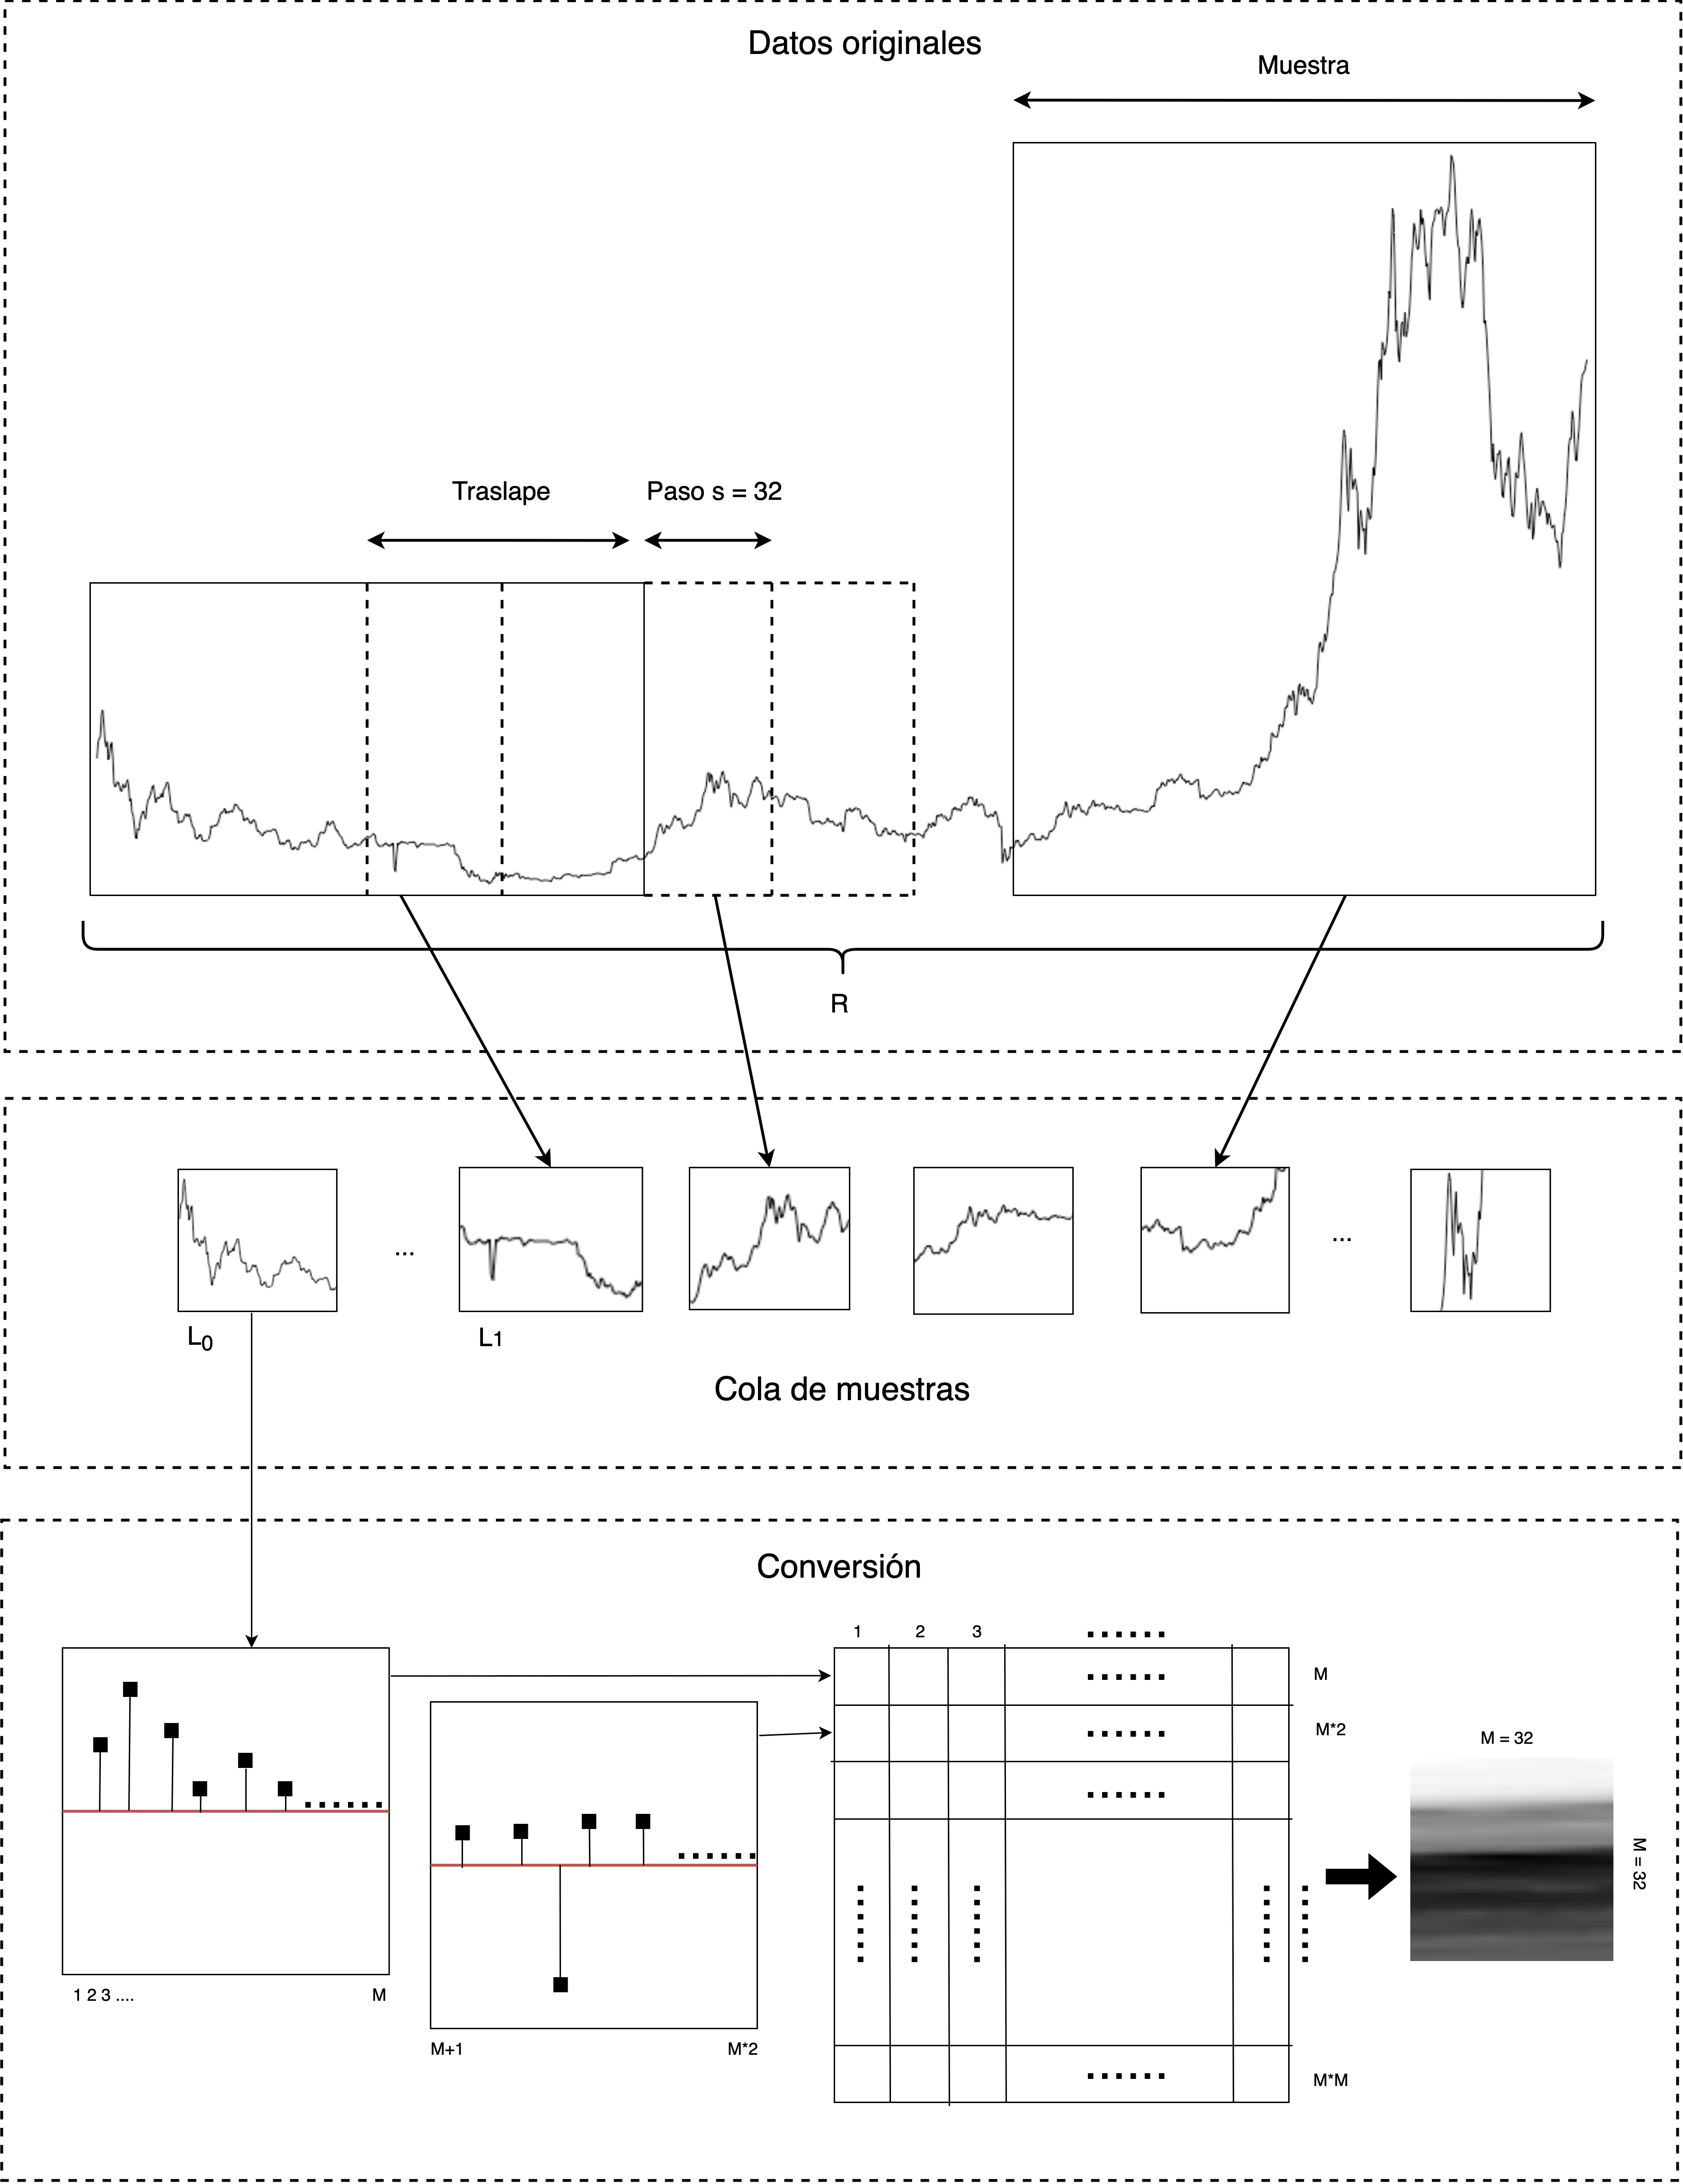
\includegraphics[width=\textwidth,height=21cm]{Chapter3/3-2.png}
	\caption{Método para convertir datos a imágenes.}
	\label{fig5}
\end{figure}

\subsection{Selección de métricas}
\label{ssec:metrics}
Para la selección de métricas que más influyen en el precio del bitcoin primero se seleccionaron aquellas que tuvieran significación estadística usando mínimos cuadrados ordinarios. De las variables seleccionadas se escogieron aquellas que tuvieran la misma dirección y el mismo o mayor peso que la variable precio usando análisis de componentes principales. Al final se corroboró la información usando un dendrograma de correlación para ver la relación entre las variables.

\subparagraph{Análisis de regresión:}
\label{AR}
Las variables endógenas que se utilizaron son las mostradas en el \autoref{tab:TableAppen1}, la variable exógena es el precio en dólares obtenido de Coin Metrics. 
A los datos de entrenamiento de las métricas se ajustó un modelo de mínimos cuadrados ordinarios de la librería statsmodels en Python y se seleccionaron las variables con un valor $p$ menor que $0.05$ con base en el estadístico $t$.


\subparagraph{Análisis de componentes principales:}
\label{PCA}

De las métricas obtenidas utilizando análisis de regresión se seleccionaron aquellas que tuvieran la misma dirección y, mayor o igual magnitud que la variable precio, para ello se utilizó la función PCA de la librería \emph{sklearn.decomposition} en Python.
Se utilizó como parámetro la cantidad total de métricas obtenidas anteriormente y se utilizó el siguiente criterio para determinar las métricas con mayor influencia en el precio
\[ F^{\prime} = \{ y \hspace{0.5mm}:\hspace{0.5mm} \lVert y \rVert_2 \geq \lVert x \rVert_2,\hspace{0.5mm} sign(y) = sign(x),\hspace{0.5mm}y \in F\} \]

donde $F$ es el conjunto de características obtenidas en el análisis de regresión, $x$ es el vector precio, $\lVert \cdot \rVert_2$ es la norma euclidiana usual y $sign$ es la función signo.

\subparagraph{Dendrograma de correlación:}
Se utilizó la función heatmap de la librería biokit en Python utilizando todas la características obtenidas en el paso anterior empleando como distancia la correlación entre las métricas y se seleccionaron aquellas que estuvieran en el mismo cluster que el precio o cercanas al mismo.

\subsection{Análisis topológico de datos}
Se siguieron los siguientes pasos para determinar los posibles crashes en el precio:

\subparagraph{Incrustar los datos en un espacio de dimensión superior:} La serie de tiempo del precio del bitcoin es incrustada en un espacio de dimensión 4 usando el teorema de Takens.
\subparagraph{Creación del panorama de persistencia:} Con los datos en un espacio de dimensión superior se calcula la homología persistente de los datos para crear el respectivo panorama de persistencia. Se utiliza la librería $TDA$ de R con la función $ripsDiag()$.
\subparagraph{Cálculo de norma topológica:} El panorama de persistencia creado en R al ser un elemento vectorial se calcula la norma L1 para después crear la norma C1 respectiva.
\subparagraph{Creación de clusters:} Se aplica el algoritmo k-means a un dataframe que tiene por columnas el logaritmo del precio del bitcoin y la norma C1 para visualizar los posibles clusters de los datos.
\subparagraph{Selección de cluster de riesgo:} En base a los siguientes criterios se selecciona el cluster que nos advierte de una posible burbuja. 

\begin{enumerate}
	\item La mayoría de los elementos del cluster cumplen que $\lVert x_t \rVert_{C1} > 0.5$
	\item Las fechas en el cluster deben ser consecutivas.
\end{enumerate}


\subsection{Fase de validación}
\subparagraph{Predicción del precio:}
En cada modelo se realizo una predicción sobre el 80\% de los datos, en estas predicciones se consideró el indicador de error RMSE (Root Mean Square Error) y la segunda versión del indice de eficiencia Theil’s U \cite{bliemelTheilForecastAccuracy1973}.
Hubo un total de 49 modelos tomando en cuenta cada transformación propuesta, de estos, el modelo seleccionado en este estudio es el que tiene menor RMSE e índice Theil’s U más cercano a cero. Con el modelo seleccionado se hace la predicción sobre el conjunto de validación como se muestra en la \autoref{subResultados}.

\begin{table}[H]
	\centering
	{
		\begin{tabular}{ll}
			\toprule
			\textbf{Indicador} & \textbf{Fórmula}\\
			\midrule
			RMSE			&$\sqrt{\frac{\sum_{i=1}^{n}({\hat{y_{n}}} - y_{n})^{2}}{n}}$\\ 
			Theil’s U 	&$\sqrt{\frac{\sum_{i=1}^{n}({\hat{y_{n}}} - y_{n})^{2}}{\sum_{i=1}^{n}y_{n}^{2}}}$ \\
			
			\bottomrule
			\hline
	\end{tabular}} \quad
	\caption{Fórmulas de los índices RMSE y Theil’s U}
	\label{tab:Table12}
\end{table}

\subparagraph{Clasificación del precio:}
Se crea un dataframe con las imágenes generadas. Una columna contiene los archivos de imagen y la otra las etiquetas de su cluster respectivo. Los clusters son renombrados a comprar, vender o incertidumbre.

Se crea el conjunto de entrenamiento del dataframe creado, se configura la CNN como en la \autoref{tab:Table11} y se entrena con los datos anteriores.

La precisión del modelo es calculada utilizando el método accuracy de tensorflow la cual crea dos variables locales, \emph{total} y \emph{count}, que se utilizan para calcular la frecuencia con la que las predicciones coinciden con las etiquetas. Esta frecuencia se devuelve finalmente como una operación que simplemente divide el total entre el recuento.






\chapter[Fundamento teórico]{Fundamento teórico}{Fundamento teórico}\label{Fundamento}

\noindent
\rule{0.49\textwidth}{0.75pt} $_{\bigcirc}$ \rule{0.49\textwidth}{0.75pt}\\

¿En que se diferencian los modelos estadísticos de los modelos de machine learning?, ¿cómo sabemos que tan bueno es un modelo?, ¿la geometría intrínseca de los datos nos puede dar información sobre eventos futuros o acaso se pueden modificar los mismos para tener una mejor comprensión de su comportamiento? Las matemáticas han demostrado ser efectivas para resolver estas preguntas que son la esencia de la predicción, la ciencia de datos y este estudio en general.
\\

\noindent
\rule{0.49\textwidth}{0.75pt} $_{\bigcirc}$ \rule{0.49\textwidth}{0.75pt}\\
\clearpage

\section{Fundamento teórico}

Los datos obtenidos de observaciones del precio del bitcoin son recolectados de forma secuencial y cronológica a lo largo del tiempo. Como ejemplo de lo anterior se puede observar diariamente el precio de apertura y cierre de este activo modelando así lo que comúnmente conocemos como serie de tiempo. En este apartado se hará una revisión breve de los modelos de predicción más utilizados en la literatura como también de análisis multivariante y análisis topológico de datos ya que son fundamentales para el estudio de series temporales, modelar los altibajos del precio y clasificar tendencias.

\section{Medidas de error}
Podemos definir al error del pronostico como la diferencia entre el valor real y el valor pronosticado de un periodo correspondiente. Unas de las medidas de error más populares son las siguientes.

\subsection{RMSE}

Root mean square error (RMSE) o raíz del error cuadrático medio representa la raíz cuadrada del segundo momento muestral de las diferencias entre valores predichos y los valores observados. Esta medida agrega las magnitudes del error en predicciones de varios puntos de datos dentro de una sola medida de predicción.
Es una medida de exactitud, para comparar errores de predicción de diferentes modelos para un conjunto de datos particular y no entre conjunto de datos ya que depende de la escala.

El RMSE es siempre no negativo, y un valor de cero podría indicar un ajuste perfecto de los datos. En general, un RMSE menor es mejor que uno alto.

\[
\operatorname{RMSE}=\sqrt{\frac{\sum_{t=1}^{T}\left(\hat{y}_{t}-y_{t}\right)^{2}}{T}}
\] 

Para valores predichos $\hat{y}_t$ para tiempos $t$ de una regresión sobre una variable dependiente $y_t$ con variables observadas $T$ veces, el RMSE es calculado $T$ veces como la raíz cuadrada de las medias de los cuadrados de las desviaciones

\subsection{MSE}

Mean Square error (MSE) o error cuadrático medio mide la media de los cuadrados de los errores, esto es, el promedio cuadrado de las diferencias entre los valores estimados y los valores reales. MSE es una función de riesgo correspondiente al valor esperado de la perdida cuadrática.

Es una medida de la calidad del estimador y es derivado del cuadrado de la distancia Euclidiana, es siempre un valor positivo que decrementa conforme el error se aproxima a cero.

Si un vector de $n$ predicciones es generado de una muestra de $n$ puntos de datos sobre todas las variables, y $Y$ es el vector de variables observadas de la variable a ser predicha, con $\hat{Y}$ siendo los valores predichos, entonces el MSE muestral del predictor es calculado como sigue 

\[
\mathrm{MSE}=\frac{1}{n} \sum_{i=1}^{n}\left(Y_{i}-\hat{Y}_{i}\right)^{2}
\]

En otras palabras, el MSE es la media de los cuadrados de los errores. 

\subsection{MAE}
Mean absolute error (MAE) o error medio absoluto es una medida de error entre observaciones emparejadas de un mismo fenómeno. Ejemplos de Y contra X incluyen la comparación de valores predichos contra observados o una técnica de medida contra otra técnica de medida. MAE se calcula como sigue

\[
\mathrm{MAE}=\frac{\sum_{i=1}^{n}\left|y_{i}-x_{i}\right|}{n}=\frac{\sum_{i=1}^{n}\left|e_{i}\right|}{n}
\] 

Esto es por tanto una media aritmética de errores absolutos $\left|e_{i}\right| = \left|y_{i}-x_{i}\right|$, donde $y_i$ es la predicción y $x_i$ el valor verdadero.

\subsection{Theil's U}

El estadístico U de Theil es una medida de exactitud relativa que compara los resultados predichos con los resultados de predecir con datos históricos mínimos. Eleva al cuadrado las predicciones para dar más peso a errores grandes y exagerados, el cual puede ayudar a eliminar métodos con errores grandes \cite{OracleCrystalBall}.

La formula para calcular el estadístico U de Theil es la siguiente

\[
U=\sqrt{\frac{\sum_{t=1}^{n-1}\left(\frac{\hat{Y}_{t+1}-Y_{t+1}}{Y_{t}}\right)^{2}}{\sum_{t=1}^{n-1}\left(\frac{Y_{t+1}-Y_{t}}{Y_{t}}\right)^{2}}}
\]

donde $Y_t$ es el valor actual de un punto para un periodo de tiempo $t$, $n$ es el numero de puntos de datos y $\hat{Y_t}$ es el valor predicho.

El estadístico se interpreta de la siguiente forma

\begin{itemize}
	\item Menor que 1 : La técnica de predicción es mejor que adivinar
	\item  Igual a 1: La técnica de predicción es igual que adivinar
	\item Mayor que 1: La técnica de predicción es peor que adivinar.
\end{itemize}

\section{Modelos estadísticos}
\label{modelosestadisticos}
Los modelos estadísticos utilizan ecuaciones matemáticas para codificar información extraída de los datos. En algunas ocasiones las técnicas de modelado estadístico pueden proporcionar modelos adecuados de forma rápida e incluso pueden ofrecer mejores resultados que algunas técnicas más flexibles de aprendizaje maquina, es posible usar algunos modelos estadísticos como modelos predictivos de línea base para juzgar el rendimiento de técnicas más avanzadas \cite{IBMDocs2021}. 

\subsection{Naive}

Para el método de predicción Naive, simplemente hacemos que el valor predicho sea igual a la última observación, esto es,

\[ \hat{y}_{T+h \mid T}=y_{T} \]

Aquí, la notación $\hat{y}_{T+h \mid T}$ es una manera corta de estimar $y_{T+h \mid T}$ basado en el los datos $y_{1}, \ldots, y_{T}$. Este método funciona bastante bien para series de tiempo económicas y financieras \cite{hyndmanForecastingPrinciplesPractice}.
Se asume que las observaciones más recientes son las más importantes y que las observaciones previas no proveen de información para el futuro.

\subsection{SES}
El método simple exponential smothing (SES) es apropiado para la predicción de datos sin una tendencia clara o sin un patrón estacional \cite{hyndmanForecastingPrinciplesPractice}. Su concepto principal es dar mayor peso a las observaciones más recientes que a las del pasado lejano, por tanto las predicciones se realizan mediante medias ponderadas, donde los pesos disminuyen de forma exponencial a medida que las observaciones son más antiguas como se observan en la \autoref{eq:1}

\begin{equation}
	\hat{y}_{T+1 \mid T}=\alpha y_{T}+\alpha(1-\alpha) y_{T-1}+\alpha(1-\alpha)^{2} y_{T-2}+\cdots
	\label{eq:1}
\end{equation}

donde $0 \leq \alpha \leq 1$ es el parámetro de suavizado. La forma de media ponderada es la siguiente:

\[\hat{y}_{T+1 \mid T}=\sum_{j=0}^{T-1} \alpha(1-\alpha)^{j} y_{T-j}+(1-\alpha)^{T} \ell_{0}\]

dónde $\ell_{0}$ es el primer valor ajustado al tiempo $t=1$, el cual tenemos que estimar y se obtiene dependiendo del tipo de error a maximizar. El valor $(1-\alpha)^{T} \ell_{0}$ tiende a $0$ si $T$ es muy grande, así que esta forma es similar a la \autoref{eq:1}. 

Una representación alternativa es la forma en componentes que está dada por:

\begin{equation*}
	\begin{array}{lcl} 
		\textrm{Ecuación de predicción} \hspace{1cm} \hat{y}_{t+h \mid t}=\ell_{t}\\
		\textrm{Ecuación de nivel}\hspace{1cm} \ell_{t}=\alpha y_{t}+(1-\alpha) \ell_{t-1},
	\end{array} 
\end{equation*}

donde $\ell_{t}$ es el nivel o valor de suavizado de la serie al tiempo $t$.  

\subsection{Holt}

Holt extendió el método SES para permitir la predicción de datos con una tendencia. Este método involucra una ecuación de predicción y dos de suavizado (una para el nivel y otra para la tendencia).

\begin{equation*}
	\begin{array}{lcl} 
		 \text {Ecuación de predicción} & \hat{y}_{t+h \mid t}=\ell_{t}+h b_{t} \\
		\text { Ecuación de nivel } & \ell_{t}=\alpha y_{t}+(1-\alpha)\left(\ell_{t-1}+b_{t-1}\right) \\
		\text { Ecuación de tendencia } & b_{t} =\beta^{*}\left(\ell_{t}-\ell_{t-1}\right)+\left(1-\beta^{*}\right) b_{t-1},
	\end{array} 
\end{equation*}

donde $\ell_{t}$ denota un estimador de nivel de la serie al tiempo $t$,  $b_{t}$ denota un estimador de la tendencia (pendiente) de la serie al tiempo $t$, $\alpha$ es el parámetro de suavizado para el nivel, $0 \leq \alpha \leq 1$ y $\beta^*$ es el parámetro de suavizado para la tendencia., $0 \leq \beta^* \leq 1$.

Como en el método SES, $\ell_{t}$ es una media ponderada de las observaciones $y_t$, en este caso $b_t$, la ecuación de tendencia es también una media ponderada sobre $\ell_{t}-\ell_{t-1}$ y $b_t$ el estimado previo de la tendencia. 

El método de Holt muestra una tendencia constante indefinida hacia el futuro tendiendo a sobre pronosticar para horizontes grandes de predicción. Dada la observación anterior Gardner y McKenzie introdujeron un parámetro de amortización que hace plana la tendencia después de un tiempo en el futuro. Se ha probado que los métodos que incluyen una tendencia amortiguada han sido más exitosos y más populares cuando las predicciones son automatizadas \cite{hyndmanForecastingPrinciplesPractice}. 

El método de Holt amortizado tiene la siguiente forma

\begin{equation*}
	\begin{array}{cl} 
	\hat{y}_{t+h \mid t} =\ell_{t}+\left(\phi+\phi^{2}+\cdots+\phi^{h}\right) b_{t} \\
	\ell_{t} =\alpha y_{t}+(1-\alpha)\left(\ell_{t-1}+\phi b_{t-1}\right) \\
	b_{t}=\beta^{*}\left(\ell_{t}-\ell_{t-1}\right)+\left(1-\beta^{*}\right) \phi b_{t-1} .
	\end{array} 
\end{equation*}

donde $\alpha$ y $\beta$ son como el método Holt y $\phi$ es el parámetro de amortización $0 \leq \phi \leq 1$.
Notemos que la ecuación de predicción converge a $\ell_{T}+\phi b_{T} /(1-\phi)$ conforme $h \rightarrow \infty$. Esto significa que las predicciones a corto plazo tienen tendencia mientras que las predicciones a largo plazo son constantes.

\subsection{ETS}

Los modelos ETS son una familia de modelos para series de tiempo que consisten en un término de error (E), un componente de tendencia (T), y un componente estacional (S) \cite{ETSModelsStatsmodels}.

La predicción con esta familia de modelos implementa todas las combinaciones de error aditivo y multiplicativo; tendencia aditiva, multiplicativa y posiblemente amortiguado; estacionalidad aditivo multiplicativo, tratado de optimizar la verosimilitud a diferencia del modelo SES o Holt.

%explicar que se uso ETS con todos los parametros en automatico para ver la mejor predicción que mejora la verosimilitud.

\subsection{ARIMA}

\subsubsection{Modelos autorregresivos}

Un modelo autorregresivo es aquel en el que predecimos la variable de interés usando una combinación lineal de valores pasados de la variable. El termino autorregresión indica que es una regresión de la variable contra sí misma \cite{hyndmanForecastingPrinciplesPractice}.

Por tanto, un modelo autorregresivo de orden $p$ puede ser escrito como 

\[ y_{t}=c+\phi_{1} y_{t-1}+\phi_{2} y_{t-2}+\cdots+\phi_{p} y_{t-p}+\varepsilon_{t} \]

donde $\varepsilon_{t}$ es ruido blanco y $y_{t-p}$ son valores retardados de $y_t$ como predictores. Esto es comúnmente conocido como \textbf{AR($p$)}.

\subsubsection{Modelo de medias móviles}

Un modelo de medias móviles usa errores de predicción pasados en una regresión, a diferencia de un modelo autorregresivo que usa valores retardados del valor a predecir \cite{hyndmanForecastingPrinciplesPractice}. Esto se puede expresar como

\[ y_{t}=c+\varepsilon_{t}+\theta_{1} \varepsilon_{t-1}+\theta_{2} \varepsilon_{t-2}+\cdots+\theta_{q} \varepsilon_{t-q} \]

donde $\varepsilon_{t}$ es ruido blanco. Esto es comúnmente conocido como \textbf{MA($q$)}, un modelo de medias móviles de orden $q$.

\subsubsection{Modelos ARIMA}

ARIMA es el acrónimo para modelo autorregresivo integrado de promedio móvil (del inglés AutoRegressive Integrated Moving Average), que es un modelo que combina la diferenciación con autorregresión y medias móviles \cite{hyndmanForecastingPrinciplesPractice}. En este caso la parte integrada del modelo hace referencia al converso de la diferenciación. 

El modelo puede ser escrito 

\[ y_{t}^{\prime}=c+\phi_{1} y_{t-1}^{\prime}+\cdots+\phi_{p} y_{t-p}^{\prime}+\theta_{1} \varepsilon_{t-1}+\cdots+\theta_{q} \varepsilon_{t-q}+\varepsilon_{t}, \]

donde $y_{t}^{\prime}$ es la serie diferenciada y los predictores de la parte izquierda de la ecuación son son valores retardados de $y_t$ y $\varepsilon_t$. Llamamos a esto un modelo \textbf{ARIMA($p,d,q$)} donde

\begin{itemize}
\item $p$ = orden de la parte autorregresiva.
\item $d$ = grado de la primer diferenciación involucrada.
\item $q$ = orden de la parte de medias móviles.
\end{itemize}

El operador $B$ (backward shift) es una notación usada para trabajar con series de tiempo retardadas

\[ B y_{t}=y_{t-1}. \]

Si aplicamos dos veces $B$ a $y_t$ entonces desplaza los datos hacia atrás dos períodos: 

\[B\left(B y_{t}\right)=B^{2} y_{t}=y_{t-2}.\]

En general este operador es particularmente útil ya que puede ser tratado usando reglas algebraicas ordinarias. También tiene la propiedad de que una diferencia de orden $d$ puede ser escrita como

\[
(1-B)^{d} y_{t}.
\]

Usando el operador $B$ podemos escribir la ecuación del modelo ARIMA de la siguiente forma

\begin{equation*}
	\begin{array}{ccc}
		\left(1-\phi_{1} B-\cdots-\phi_{p} B^{p}\right) & (1-B)^{d} y_{t}=c+\left(1+\theta_{1} B+\cdots+\theta_{q} B^{q}\right) \varepsilon_{t}\\
		\hspace{0.5cm}\uparrow & \hspace{-5cm}\uparrow & \hspace{-7cm}\uparrow \\
		\operatorname{AR}(p) & \hspace{-5cm}d\hspace{0.1cm}\text{diferencias} & \hspace{-7cm}\operatorname{MA}(q)
	\end{array}
\end{equation*}
\section{Transformaciones matemáticas}
\label{transformacionesmatematicas}
Ajustar los datos en algunos casos puede mejorar la predicción de los mismos ya que permiten disminuir la variabilidad o simplificar los patrones o tendencias de los registros históricos. En este estudio se aplicaron trasformaciones matemáticas para generar series de tiempo que refuerzan la tendencia o hacerla estacionaria.


\subsection{Transformación $\log$}

Si denotamos las observaciones originales como $y_{1}, \ldots, y_{T}$ y las observaciones transformadas como $w_{1}, \ldots, w_{T}$, entonces $w_{t}=\log \left(y_{t}\right)$. Los logaritmos son útiles dado que son interpretables. Por ejemplo, si $\log$ base 10 es usada entonces un incremento de 1 en la escala logarítmica significa una multiplicación de 10 en la escala original.  
Otra propiedad útil es que restringe la predicción a permanecer positiva en la escala original. 

\subsection{Transformación Box-Cox}
La familia de transformaciones Box-Cox que dependen del parámetro $\lambda$ se define como sigue

\[
w_{t}= \begin{cases}\log \left(y_{t}\right) & \text { if } \lambda=0 \\ \left(y_{t}^{\lambda}-1\right) / \lambda & \text { otro caso }\end{cases}
\]

Esta transformación abarca la transformación logarítmica y de potencias, si $\lambda = 0$ entonces el logaritmo natural es usado si no se usa una trasformación de potencias con un escalamiento.

La ventaja de esta transformación es que tomando un buen valor de $\lambda$ podemos estabilizar la varianza en toda la serie de tiempo, haciendo el modelo de predicción más simple \cite{hyndmanForecastingPrinciplesPractice}. 

\subsection{Transformación diff}

La diferencia en series es el cambio entre observaciones consecutivas en la serie original y puede ser escrita de la siguiente manera

\[
y_{t}^{\prime}=y_{t}-y_{t-1}
\]

Una de las ventajas de esta transformación es que puede ayudar a estabilizar la media de una serie de tiempo al eliminar los cambios de nivel de la misma y, por tanto, eliminar (o reducir) la tendencia y la estacionalidad \cite{hyndmanForecastingPrinciplesPractice}.

\subsection{Transformación diff($\log$)}

La transformación diff($\log$) calcula cambios relativos, esto es, la diferencia fraccional entre dos números que, multiplicado por cien es la diferencia porcentual entre los mismos. Estos cambios son simétricos y útiles para explorar las relaciones con datos continuos y de valor positivo \cite{coleStatisticsNotesPercentage2017}.

\[
y_{t}^{\prime}=\log{y_{t}}-\log{y_{t-1}}
\]

En finanzas esta transformación puede ser usada para analizar el cambio porcentual de la tendencia.


\section{Modelos de machine learning}
\label{modelosmachinelearning}
Un modelo de machine learning es una expresión de un algoritmo que analiza gran cantidad de datos para encontrar patrones o realizar predicciones. Los modelos de ML son los motores matemáticos de la IA.
Un modelo de machine learning es una representación matemática de los objetos y sus relaciones entre sí. Los objetos pueden ser cualquier cosa, ya sea un "me gusta'' en una publicación de redes sociales hasta moléculas en un experimento de laboratorio \cite{parsonsQueEsModelo2021}.

\subsection{RTS}
El modelo de regresión sobre series de tiempo (RTS) es una variación de los modelos de regresión lineal que permite agregar variables para la tendencia y temporada \cite{TslmFitLinear}. 

La forma general de un modelo de regresión lineal multiple es la siguiente:

\[
y_{t}=\beta_{0}+\beta_{1} x_{1, t}+\beta_{2} x_{2, t}+\cdots+\beta_{k} x_{k, t}+\varepsilon_{t}
\]

donde $y$ es la variable a predecir y $x_{1}, \ldots, x_{k}$ son las $k$ variables predictoras.
Los coeficientes $\beta_{1}, \ldots, \beta_{k}$ miden el efecto de cada predictor después de tener en cuenta los efectos de todos los demás predictores del modelo.

Las suposiciones implícitas que se hacen al aplicar un modelo de regresión lineal son las siguientes:

\begin{itemize}
\item La relación entre la variable de pronóstico y las variables predictoras satisfacen una ecuación lineal.
\item Los errores tienen media cero.
\item Los errores no están autocorrelacionados.
\item Los errores no están correlacionados con las variables predictoras.
\end{itemize}

Otra suposición importante es que cada predictor no sea una variable aleatoria ya que deben ser datos reproducibles. Con datos observacionales (como la mayoría de datos financieros) no es posible controlar el comportamiento de los datos ya que simplemente son observados, por tanto se hace la suposición de que no son una variable aleatoria y pueden ser controlados para hacer regresión sobre ellos \cite{hyndmanForecastingPrinciplesPractice}.

La variable tendencia del modelo RTS puede ser modelada usando $x_{1, t}=t$ como predictor.

\[
y_{t}=\beta_{0}+\beta_{1} t+\varepsilon_{t}
\]

donde $t=1,...,T$. Por otra parte la temporada se modela agregando variables ficticias para codificar categorías. Cada categoría corresponde a una ventana de tiempo. Estas variables ficticias miden el efecto de la categoría relativa a la categoría omitida \cite{hyndmanForecastingPrinciplesPractice}. 

\subsection{SVM}

Support vector machines (SVM) es un algoritmo de machine learning supervisado que se basa en separar los puntos de los datos usando hiperplanos tal que la distancia de separación es máxima. Los vectores de soporte son los puntos más cercanos al hiperplano para calcular su posición \cite{mudassirTimeseriesForecastingBitcoin2020}.
Para el cálculo de los SVM la función objetivo \ref{svm} debe ser minimizada sujeto a la condición \ref{svm_restric}.

\begin{equation}
	\|\mathbf{w}\|^{2}+C \sum_{i=1}^{n} \zeta_{i}
	\label{svm}
\end{equation}

En la \autoref{svm} la variable de holgura es $\zeta_{i}$, la penalización es $C$ y $\mathbf{w}$ es la normal al hiperplano.

\begin{equation}
	y_{i}\left(\mathbf{w} \cdot \phi\left(x_{i}\right)+b \right) \geq 1-\zeta_{i}, \quad \text { con } \zeta_{i} \geq 0.
	\label{svm_restric}
\end{equation}

En la restricción \ref{svm_restric} $x_i$ y $y_i$ son puntos en los datos y $\phi(x_i)$ son los datos transformados. 

En datos no lineales generalmente no es posible encontrar un hiperplano de separación lineal, para solucionar este problema usamos el truco del kernel. La idea básica detrás de esto es que cuando el conjunto de datos no es separable en la dimensión actual, entonces agregamos otra dimensión y probar si los datos son separables.
Estas transformaciones que nos ayudan a agregar niveles de diferencia a los datos son llamadas kernels. Los más populares son los siguientes: kernel polinomial, kernel gaussiano, función base radial (RBF), kernel Laplace RBF, kernel sigmoide, anove RBF, etc.  

Análogamente existe una versión de regresión del algoritmo SVM que consiste en resolver el siguiente problema

\[
\begin{array}{r@{}r@{}r@{}l}
	\text{Min} \quad \frac{1}{2}\|w\|^{2} \\[\jot]
	\text{s.t.}\qquad \left|y_{i}-\left\langle w, x_{i}\right\rangle-b\right| \leq \varepsilon \\
	
\end{array}
\]

donde $x_i$ es una muestra de entrenamiento con valor objetivo $y_i$. Aquí $\left\langle w, x_{i}\right\rangle+b$ es la predicción y $\epsilon$ es un parámetro libre que sirve como umbral. Todas las predicciones tienen que estar dentro de un rango $\epsilon$ de predicciones verdaderas. 

\subsection{Random Forest}
El algoritmo de bosque aleatorio o random forest combina la salida de múltiples arboles de decisión tal que cada árbol depende de los valores de un vector aleatorio probado independientemente y con la misma distribución para cada uno de estos y así alcanzar un solo resultado. Es usado para problemas de regresión y clasificación \cite{WhatRandomForest2021}.

\subsubsection{Árboles de decisión}
Un árbol de decisión divide una pregunta inicial en subpreguntas para llegar a una decisión final. Observaciones que se ajusten a un criterio seguirán una rama "sí", y aquellas que no, seguirán un camino distinto.

Entonces un árbol de decisión busca encontrar la mejor partición de un subconjunto de los datos y estos generalmente son entrenados con el algoritmo Classification and Regression Tree (CART).
Las métricas usadas para evaluar la calidad de las particiones son Gini impurity, information gain, o MSE.   

\subsubsection{Métodos de conjunto (Ensamble methods)}

Los métodos de conjunto son técnicas que buscan mejorar la precisión de resultados en modelos combinando múltiples modelos en vez de usar uno solo. Los modelos de conjunto más populares son: bagging, boosting y staking.
En el método bagging se selecciona una muestra aleatoria de datos en un conjunto de entrenamiento con remplazo, significando esto que los datos se pueden elegir más de una vez. Después de generar varias muestras de los datos estos se entrenan de forma independiente ya sea regresión o clasificación. El promedio o mayoría de de esas predicciones nos levan a una mejor precisión.   

\subsubsection{Algoritmo random forest}

El algoritmo random forest es una exención del método baggin ya que utiliza tanto el baggig como la selección aleatoria de características para crear un bosque no correlacionado de arboles de decisión.
La aleatoriedad de características, también conocida como bagging de características o ''el método del subespacio aleatorio'' es la diferencia clave entre los bosques aleatorios y los arboles de decisión ya que mientras los arboles de decisión consideran todas las posibles divisiones de características, los bosques aleatorios solo seleccionan un subconjunto de ellas.


\subsection{LSTM}

Long Short-term memory (LSTM) constituye un caso especial de una red neuronal convolucional, la cual fue propuesta para modelar dependencias a corto y largo plazo. Este modelo de deep learnig es especialmente útil para modelado y predicción de datos de series de tiempo \cite{mudassirTimeseriesForecastingBitcoin2020}.
Una unidad LSTM consiste en una memoria de celda que almacena información y es actualizada por tres puertas principales: la puerta de entrada, la puerta de olvido y la puerta de salida \cite{chenBitcoinPricePrediction2020}.
En cada paso $t$ la puerta de entrada $i_t$ determina que información es agregada a la celda de estado $S_t$ (memoria), la puerta de olvido $f_t$ determina que información es desechada de la celda de estado mediante la decisión de una función de transformación en la capa de la puerta de olvido, mientras que la puerta de salida $o_t$ determina qué información del estado de la celda se utilizará como salida \cite{livierisEnsembleDeepLearning2020}.
En en bloque LSTM, $C_{t-1}$ es la memoria o celda de estado del bloque anterior, $h_{t-1}$ es la salida del bloque anterior, $X_t$ es el vector de entrada, $C_t$  es la memoria o celda de estado del bloque presente y  $h_{t}$ es la salida del bloque actual.
Las puertas y celdas de estado LSTM están dadas por las ecuaciones \ref{LSTM1} a \ref{LSTM2}.

\begin{equation}
	f_{t}=\sigma_{g}\left(W_{f} x_{t}+U_{f} h_{t-1}+b_{f}\right)
	\label{LSTM1}
\end{equation}

donde $f_t$ es el vector de activación de la puerta de olvido, $W$ y $U$ son matrices ponderadas, $b$ es el vector de sesgo y $\sigma_{g}$ es la función sigmoide. 

\begin{equation}
	i_{t}=\sigma_{g}\left(W_{i} x_{t}+U_{i} h_{t-1}+b_{i}\right)
\end{equation}

donde $i_t$ es el vector de activación de la puerta de entrada o activación.

\begin{equation}
	o_{t}=\sigma_{g}\left(W_{o} x_{t}+U_{o} h_{t-1}+b_{o}\right)
\end{equation}

donde $o_t$ es el vector de activación de la puerta de salida.

\begin{equation}
	\tilde{c}_{t}=\sigma_{h}\left(W_{c} x_{t}+U_{c} h_{t-1}+b_{c}\right)
\end{equation}

donde el vector de activación de la celda de entrada está dada por $c_t$ y $\sigma_{h}$ es la función tangente hiperbólica.

\begin{equation}
	c_{t}=f_{t} \otimes c_{t-1}+i_{t} \otimes \tilde{c}_{t}
\end{equation}

donde $c_t$ es el estado de la celda o vector memoria.

\begin{equation}
	h_{t}=o_{t} \otimes \sigma_{h}\left(c_{t}\right)
	\label{LSTM2}
\end{equation}

donde $h_t$ es el vector de salida del bloque LSTM o el vector de estado oculto. 


\subsection{CNN}
Una red neuronal convolucional o convolutional neural network (CNN) es una red neuronal de aprendizaje profundo diseñada para procesar arreglos estructurados de datos, tales como imágenes. Las redes neuronales convolucionales se han convertido en el estado del arte de varias aplicaciones visuales como clasificación de imágenes \cite{ConvolutionalNeuralNetwork2019}.

Las redes neuronales convolucionales son muy buenas captando patrones de la imagen de entrada, tales como líneas, gradientes, círculos, incluso ojos y caras. A diferencia de los primeros algoritmos de visión por computadora, las redes neuronales convolucionales pueden operar directamente sobre una imagen pura, sin modificar. El poder de estas redes viene de una especia de capa especial llamada la capa de convolución \cite{ConvolutionalNeuralNetwork2019}.

Podemos visualizar una capa de convolución como varias pequeñas plantillas cuadradas llamadas kernels convolucionales, las cuales se deslizan sobre la imagen y buscan por patrones. Donde esa parte de la imagen coincide con el patrón del kernel, el kernel retorna un valor grande positivo, y cuando no coincide retorna cero o un valor muy pequeño.

Para llevar a cabo la convolución, deslizamos el kernel de convolución sobre la imagen. En cada posición, multiplicamos cada elemento del kernel de convolución por el elemento de la imagen que cubre y sumamos los resultados. Supongamos que el kernel es de $3\times3$ y la imagen es de $9\times 9$ entonces la imagen resultante es de $7\times 7$, ya que el kernel solo puede ser deslizado sobre la imagen siete veces.

En práctica, un kernel de convolución contiene pesos y sesgos, similar a la fórmula de regresión lineal. Así, un pixel de entrada es multiplicado por un peso y entonces un sesgo es agregado.

Después de que una imagen pase a través de una capa de convolución, la salida normalmente pasa a través de una función de activación. Funciones de activación comunes incluyen la función sigmoide

\[
S(x)=\frac{1}{1+e^{-x}}
\]

y la función ReLu, también conocida como la unidad lineal rectificadora

\[
f(x)=\max (0, x)
\]
 
La función de activación tiene el efecto de agregar no linealidad a la red neuronal convolucional. Si la función de activación no estuviera presente, todas las capas de la red neuronal podrían condensarse en una sola matriz de multiplicación. En el kernel anterior, aplicar una función de activación ReLu podría significar un mayor contraste.

Una red neuronal convolucional básica puede ser vista como una serie de capas convolucionales, seguidas de una función de activación, seguidas por una capa pooling (reducción de escalado tomando un conjunto de píxeles y creado uno nuevo con el promedio de los mismos) repetido varias veces.
 

\subsection{K-Means}

El algoritmo K-means es un algoritmo de partición con la meta de asignar a cada punto de dato un único agrupamiento. Divide un conjunto de $n$ muestras $X$ dentro de $k$ agrupamientos disjuntos $c_i$, $i=1,...,k$, cada uno descrito por la media $\mu_i$ de las muestras en el agrupamiento. Las medias son comúnmente llamados centroides del agrupamiento. El algoritmo K-means asume que todos los $k$ grupos tienen la misma varianza \cite{igualIntroductionDataScience2017}.

El agrupamiento K-means resuelve el siguiente problema de minimización. 

\begin{equation}
	\arg \min _{c} \sum_{j=1}^{k} \sum_{x \in c_{j}} d\left(x, \mu_{j}\right)=\arg \min _{c} \sum_{j=1}^{k} \sum_{x \in c_{j}}\left\|x-\mu_{j}\right\|_{2}^{2}
\end{equation}

donde $c_i$ es el conjunto de puntos que pertenecen al agrupamiento $i$ y $\mu_i$ es el centro de la clase $c_i$. La función objetivo del agrupamiento K-means usa el cuadrado de la distancia Euclidiana $d\left(x, \mu_{j}\right)=\left\|x-\mu_{j}\right\|^{2}$ que también es conocida como inercia.
%Pág. 121 de libro de Zotero zotero://select/library/items/I2TMXUMY

\section{Análisis de regresión}
La regresión esta relacionada a como hacemos predicciones de cantidades del mundo real, las predicciones hacen referencia a preguntas que tienen una estructura en común: se preguntan por una respuesta que puede ser expresada como una combinación de una o más variables (independientes) que también son llamadas covariables o predictores. El papel de la predicción es construir un modelo para predecir la respuesta de las variables y que puede ser útil en diferentes tareas, (1) analizar el comportamiento de los datos, (2) predecir los valores de los datos y (3) encontrar variables importantes para el modelo \cite{igualIntroductionDataScience2017}.
%zotero://select/library/items/I2TMXUMY
\subsection{Mínimos cuadrados ordinarios}

Mínimos cuadrados ordinarios es un método estadístico para estimar parámetros desconocidos en un modelo de regresión lineal \cite{juarez4toColoquioDepartamento}. Entonces sea $x$ una variable independiente y sea $y(x)$ una función desconocida de $x$ la cual queremos aproximar. Suponiendo que tenemos $m$ observaciones

\[
\left(x_{1}, y_{1}\right),\left(x_{2}, y_{2}\right), \ldots,\left(x_{m}, y_{m}\right)
\]

donde $y_i \sim y(x_i)$, $i=1,...,m$, la idea es modelar $y(x)$ por medio de una combinación de $n$ funciones base $\phi_1(x),\phi_2(x),...\phi_n(x)$. En el caso lineal suponemos que la función se ajusta a los datos en una combinación lineal de la forma 

\[
y(x)=c_{1} \phi_{1}(x)+c_{2} \phi_{2}(x)+\ldots+c_{n} \phi_{n}(x)
\]

Entonces, los datos deben satisfacer de manera aproximada

\[
y_{i}=c_{1} \phi_{1}\left(x_{i}\right)+c_{2} \phi_{2}\left(x_{i}\right)+\ldots+c_{n} \phi_{n}\left(x_{i}\right), \quad i=1,2, \ldots, m
\]

La ecuación anterior puede expresarse de forma matricial como sigue

\[
\left[\begin{array}{cccc}
	\phi_{1}\left(x_{1}\right) & \phi_{2}\left(x_{1}\right) & \ldots & \phi_{n}\left(x_{1}\right) \\
	\phi_{1}\left(x_{2}\right) & \phi_{2}\left(x_{2}\right) & \ldots & \phi_{n}\left(x_{2}\right) \\
	\vdots & & \ddots & \vdots \\
	\phi_{1}\left(x_{m}\right) & \phi_{2}\left(x_{m}\right) & \ldots & \phi_{n}\left(x_{m}\right)
\end{array}\right]\left[\begin{array}{c}
	c_{1} \\
	c_{2} \\
	\vdots \\
	c_{n}
\end{array}\right]=\left[\begin{array}{c}
	y_{1} \\
	y_{2} \\
	\vdots \\
	y_{m}
\end{array}\right]
\]

El enfoque de mínimos cuadrados consiste en buscar aquel vector de coeficientes $c$ que minimice el residual $r=y-Ac$. Entonces, el problema consiste en resolver 

\[
\min _{c \in \mathbb{R}^{n}}\|A c-y\|^{2}
\]

Es decir, para encontrar el ajuste de mínimos cuadrados debemos encontrar el vector de coeficientes $c=(c_1,...,c_n)^T$ que minimiza la suma de los cuadrados:

\[
\min _{c \in \mathbb{R}^{n}} \sum_{i=1}^{m}\left(c_{1} \phi_{1}\left(x_{i}\right)+c_{2} \phi_{2}\left(x_{i}\right)+\cdots+c_{n} \phi_{n}\left(x_{i}\right)-y_{i}\right)^{2}.
\]

%zotero://select/library/items/I2TMXUMY
%zotero://select/library/items/PQ8TC77F
\section{Análisis de componentes principales}

La idea principal del análisis de componentes principales (PCA) es reducir la dimensionalidad de un conjunto de datos con variables que están interrelacionados entre sí, mientras retienen la mayor variación posible. Esto se logra transformándolas a un nuevo conjunto de variables, los componentes principales (PCs), las cuales no están relacionadas y están ordenadas de tal forma que las primeras tienen la mayor variación presente de todas las variables originales \cite{jolliffePrincipalComponentAnalysis2002}.

Supongamos que $x$ es un vector de $p$ variables aleatorias y que la varianza de las $p$ variables aleatorias y la estructura de la covarianza o correlación entre las $p$ variables es de interés. El primer paso del PCA es buscar una función lineal $\boldsymbol{\alpha}_1^\prime \boldsymbol{x}$ de los elementos de $\boldsymbol{x}$ que tenga máxima varianza, donde $\boldsymbol{\alpha}_{1}$ es un vector de $p$ constantes $\alpha_{11},\alpha_{12},...,\alpha_{1p}$ y $\prime$ denota la traspuesta, así que

\[
\boldsymbol{\alpha}_{1}^{\prime} \boldsymbol{x}=\alpha_{11} x_{1}+\alpha_{12} x_{2}+\cdots+\alpha_{1 p} x_{p}=\sum_{j=1}^{p} \alpha_{1 j} x_{j}
\] 

Consideremos de momento que el vector de variables aleatorias $\boldsymbol{x}$ tiene una matriz de covarianza conocida $\boldsymbol{\Sigma}$, esta es la matriz cuya $(i,j)$-ésimos elementos es la covarianza conocida entre el $i$-ésimo y $j$-ésimo elemento de $\boldsymbol{x}$ cuando $i \neq j$ y la varianza del $j$-ésimo elemento de $\boldsymbol{x}$ cuando $i = j$. Resulta que para $k=1,2,..,p$ el $k$-ésimo PC está dado por $z_k = \boldsymbol{\alpha_k^\prime} \boldsymbol{x}$ donde $\boldsymbol{\alpha_k}$ es un eigenvector de $\boldsymbol{\Sigma}$ correspondiente al $k$-ésimo eigenvalor más grande $\lambda_k$. Aún más, si $\boldsymbol{\alpha_k^\prime}$ es escogido de tal forma que tiene longitud unidad $(\boldsymbol{\alpha_k^\prime}\boldsymbol{\alpha_k}=1)$, entonces la $var(z_k)=\lambda_k$, donde $var(z_k)$ denota la varianza de $z_k$.

Para derivar la forma de los PC, consideremos primero $\boldsymbol{\alpha_k^\prime}$ donde $\boldsymbol{\alpha_k}$ maximiza $var(\boldsymbol{\alpha_k^\prime})= \boldsymbol{\alpha}_{1}^{\prime} \boldsymbol{\Sigma} \boldsymbol{\alpha}_{1}$. Entonces el problema a resolver es el siguiente:
\[
\begin{array}{r@{}r@{}r@{}l}
	\text{Max} \quad \boldsymbol{\alpha}_{1}^{\prime} \boldsymbol{\Sigma} \boldsymbol{\alpha}_{1} \\[\jot]
	\text{s.t.}\qquad \boldsymbol{\alpha_k^\prime}\boldsymbol{\alpha_k}=1 \\
	
\end{array}
\]

Usando la técnica de los multiplicadores de Lagrange obtenemos que el eigenvalor $\lambda$ de $\boldsymbol{\Sigma}$ con $\boldsymbol{\alpha}_{1}$ su correspondiente eigenvector. Para decidir cual de los $p$ eigenvectores da $\boldsymbol{\alpha}_{1}^{\prime}\boldsymbol{x}$ con máxima varianza, notemos que la cantidad a ser maximizada es la siguiente

\[
\boldsymbol{\alpha}_{1}^{\prime} \boldsymbol{\Sigma} \boldsymbol{\alpha}_{1}=\boldsymbol{\alpha}_{1}^{\prime} \lambda \boldsymbol{\alpha}_{1}=\lambda \boldsymbol{\alpha}_{1}^{\prime} \boldsymbol{\alpha}_{1}=\lambda,
\]

así $\lambda$ debe ser tan grande como sea posible. Por tanto, $\boldsymbol{\alpha}_{1}$ es el eigenvector correspondiente al eigenvalor más grande de $\boldsymbol{\Sigma}$ y $\operatorname{var}\left(\boldsymbol{\alpha}_{1}^{\prime} \mathbf{x}\right)=\boldsymbol{\alpha}_{1}^{\prime} \boldsymbol{\Sigma} \boldsymbol{\alpha}_{1}=\lambda_{1}$, es el eigenvalor más grande.
En general el $k$-ésimo PC de $\boldsymbol{x}$ es $ \boldsymbol{\alpha_k^\prime} \boldsymbol{x}$ y $var(\boldsymbol{\alpha_k^\prime}\boldsymbol{x})=\lambda_k$ donde $\lambda_k$ es el $k$-ésimo eigenvalor más grande de $\boldsymbol{\Sigma}$, y $\boldsymbol{\alpha_k}$ es el correspondiente eigenvector.

Los vectores de los coeficientes $\boldsymbol{\alpha}_{3}, \boldsymbol{\alpha}_{4}, \ldots, \boldsymbol{\alpha}_{p}$, son los eigenvectores de $\boldsymbol{\Sigma}$ correspondiente a $\lambda_{1},\lambda_{2},...,\lambda_{p}$.

\[
\operatorname{var}\left[\boldsymbol{\alpha}_{k}^{\prime} \mathbf{x}\right]=\lambda_{k} \quad \text { para } k=1,2, \ldots, p
\]

La derivación de los coeficientes PC y varianzas como eigenvectores y eigenvalores de una matriz de covarianza es estándar. 

\section{Agrupamiento jerárquico}
El agrupamiento jerárquico es un método de análisis de grupos puntuales el cual busca construir una jerarquía de grupos.
Hay dos estrategías para el agrupamiento jerárquico:
\begin{itemize}
	\item Aglomerativas: Este es un acercamiento ascendente, cada observación comienza en su propio grupo, y los pares de grupos son mezclados mientras uno sube en la jerarquía.
	\item Divisivas: Este es un acercamiento descendente, todas las observaciones comienzan en un grupo, y se realizan divisiones mientras uno baja en la jerarquía.
\end{itemize}

Los resultados de un agrupamiento jerárquico son usualmente presentados en un dendrograma. 

En orden de decidir qué grupos deberían ser combinados, o cuando un grupo debería ser dividido, una medida de disimilitud entre conjuntos de observaciones es requerida y un criterio de enlace el cual especifica la disimilitud de conjuntos como una función de las distancias dos a dos entre observaciones en los conjuntos.

Algunas métricas usualmente usadas para el agrupamiento jerárquico son las mostradas en la \autoref{tab:metricsDendrograma}.

\begin{table}[h]
	\centering
	\begin{tabular}{m{6cm} m{6cm}  }
		\toprule
		\textbf{Nombre} & \textbf{Fórmula}\\
		\midrule
		 Distancia euclidiana & $\|a-b\|_{2}=\sqrt{\sum_{i}\left(a_{i}-b_{i}\right)^{2}}$\\
		\hline 
		Distancia euclidiana al cuadrado & $\|a-b\|_{2}^{2}=\sum_{i}\left(a_{i}-b_{i}\right)^{2}$ \\
		\hline 
		Distancia Manhattan & $\|a-b\|_{1}=\sum_{i}\left|a_{i}-b_{i}\right|$ \\
		\hline 
		Distancia máxima & $\|a-b\|_{\infty}=\max _{i}\left|a_{i}-b_{i}\right|$ \\
		\hline 
		Distancia de Mahalanobis & $\sqrt{(a-b)^{\top} S^{-1}(a-b)}$ donde $S$ es la matriz de covarianza \\
		\hline 
		Similitud coseno & $\frac{a \cdot b}{\|a\| b \|}$ \\
		\bottomrule
		\hline
	\end{tabular}
	\caption{Distancias usuales entre conjuntos de observaciones.}
	\label{tab:metricsDendrograma}
\end{table}



El criterio de enlace determina la distancia entre conjuntos de observaciones como una función de las distancias entre observaciones dos a dos. Algunos criterios de enlace entre dos conjuntos de observaciones A y B frecuentemente usados son las mostradas en \autoref{tab:critEnlance}

\begin{table}[h]
	\centering
	\begin{tabular}{m{8cm} m{8cm}  }
		\toprule
		\textbf{Nombre} & \textbf{Fórmula}\\
		\midrule
		Agrupamiento de máximo o completo enlace & $\max \{d(a, b): a \in A, b \in B\}$ \\
		\hline
		Agrupamiento de mínimo o simple enlace & $\min \{d(a, b): a \in A, b \in B\}$ \\
		\hline
		Agrupamiento de enlace media o promedio & $\frac{1}{|A||B|} \sum_{a \in A} \sum_{b \in B} d(a, b)$ \\
		\hline
		Agrupamiento de mínima energía & \parbox[t]{8cm}{
			$\frac{2}{n m} \sum_{i,j=1}^{n,m}\left\|a_{i}-b_{j}\right\|_{2} -
			\frac{1}{n^{2}} \sum_{i,j=1}^{n}\left\|a_{i}-a_{j}\right\|_{2}-
			\frac{1}{m^{2}} \sum_{i, j=1}^{m}\left\|b_{i}-b_{j}\right\|_{2}$
		} \\
		\bottomrule
		\hline
	\end{tabular}
	\caption{Distancias usuales entre conjuntos de observaciones.}
	\label{tab:critEnlance}
\end{table}

donde $d$ es la métrica escogida. Otros criterios de enlace incluyen pueden ser: la suma de todas las varianzas del intragrupo, el decrecimiento en la varianza para los grupos que están siendo mezclados (criterio de Ward) o la probabilidad de que grupos candidatos se produzcan desde la misma función de distribución (V-enlace).

\section{Análisis topológico de datos}

El análisis topológico de datos es una herramienta matemática para estudiar la estructura y forma de los datos, esta involucra elementos de topología algebraica, cómputo, y probabilidad y estadística. 
La entrada de este método es un conjunto de datos de nube de puntos, al cual, una forma geométrica representada por un complejo simplicial es asociada. La información topológica de esa forma es extraída en términos de homología de grupos. La salida del método es una diagrama de persistencia o panorama de persistencia, el cual representa un resumen de todas las características topológicas mostradas por los datos clasificados por un parámetro escalar. Los panoramas de persistencia son elementos de cierto espacio de Banach de funciones lineales a trozos, por tanto tienen normas asociadas \cite{gideaTopologicalRecognitionCritical2020}.

El foco en criptomonedas es motivado por las propiedades de sus correspondientes series de tiempo, ya sea la falta de estacionalidad, que tengan memoria a largo plazo, o alta volatilidad. Tales características hacen a las criptomonedas un caso ideal de aplicación de TDA, el cual es libre de suposiciones estadísticas \cite{gideaTopologicalRecognitionCritical2020}.

\subsection{Teorema de Takens}

La incrustación de coordenadas con retardo de tiempo es un procedimiento estándar para reconstruir el espacio fase de un sistema dinámico no lineal de una serie de tiempo. Entonces, dado un sistema dinámico discreto definido por un diffeomorfismo $f:M \to M$ en una variedad $M$ $D$-dimensional, la evolución del estado $p\in M$ es dado por su órbita $\{f^{\prime}(p):t\in \mathbb{Z}\}$. Para un observable $\phi:M \to \mathbb{R}$ del sistema, uno define un conjunto reconstruido $\mathcal{A}^d$ consistiendo de vectores $d$-dimensionales de la forma  

\[
\left(\phi(p), \phi(f(p)), \ldots, \phi\left(f^{d-2}(p)\right), \phi\left(f^{d-1}(p)\right)\right)
\]

los cuales son obtenidos de evaluaciones sucesivas de $\phi$ a lo largo de segmentos de órbita

\[
\left\{p, f(p), \ldots, f^{d-2}(p), f^{d-1}(p)\right\}.
\]

Asume que $f,\phi$ son $C^r$-diferenciable con $r\geq 2$. El teorema clásico de Takens dice que, si $d\geq 2D$ entonces para conjuntos genéricos ($C^1$-abierto y denso) de $f$ y $\phi$, el mapeo $\Phi$ dado por

\[
p \in M \stackrel{\Phi}{\mapsto}\left(\phi(p), \phi(f(p)), \ldots, \phi\left(f^{d-2}(p)\right), \phi\left(f^{d-1}(p)\right)\right) \in \mathbb{R}^{d}
\]

es un inscrustamiento. Además el mapeo $f$ sobre $M$ es topológicamente conjugado con el mapeo left-shift $\sigma$ sobre el conjunto reconstruido $\mathcal{A}^d$, el cual es definido por

\[
\left(\phi(p), \ldots, \phi\left(f^{d-2}(p)\right), \phi\left(f^{d-1}(p)\right)\right) \stackrel{\sigma}{\mapsto}\left(\phi(f(p)), \ldots, \phi\left(f^{d-1}(p)\right), \phi\left(f^{d}(p)\right)\right)
\]

donde la conjugación topológica significa que $\Phi$ hace coincidir órbitas de $f$ con órbitas de $\sigma$, es decir $\sigma \circ \Phi = \Phi \circ f$.
   
\subsection{Complejo simplicial}

La entrada del método es una nube de puntos, es decir, una colección finita de puntos de datos incrustados en algun espacio Euclidiano. Consideremos una nube de puntos ${Z^t} \subseteq  \mathbb{R}^{d}$, para simplificar la notación fijemos tal nube de puntos y denotemosla por $Z=\{z_0,z_1,...,z_{w-1}\}$. Asociamos $Z$ a un espacio topológico como sigue. Se introduce un parámetro escalar $\epsilon > 0$ y definimos lo que llamaremos como complejo simplicial Vietoris-Rips $R(Z,\epsilon)$ como sigue

Para cada $k=0,1,...,$ un $k$-simplex de vertices $\{ z_{i_0},z_{i_1},...,z_{i_k} \}$ es parte de $R(Z,\epsilon)$ si y sólo si la distancia mutua entre cualquier par de vertices es menor que $\epsilon$, esto es

\[
d\left(z_{i_{j}}, z_{i_{l}}\right)<\varepsilon, \forall z_{i_{j}}, z_{i_{l}} \in\left\{z_{i_{0}}, \ldots, z_{i_{k}}\right\}
\]

En otras palabras, un $k$-simplex es incluido en $R(Z,\epsilon)$ siempre que los vertices de ese simplex sean indistinguibles uno del otro en el nivel $\epsilon$ del parametro de escala.

\subsection{Filtración de Rips y nacimiento y muerte de características topológicas}

Los complejos simpliciales de Rips $R(Z,\epsilon)$ forman una filtración, esto es, $R(Z,\epsilon) \subseteq R(Z,\epsilon^{\prime})$ siempre que $\epsilon < \epsilon^{\prime} $. Para cada tal complejo podemos calcular su homología $n$-dimensional $H_n(R(Z,\epsilon))$ con coeficientes en algún campo. Los generadores del grupo de homología $0$-dimensional $H_0(R(Z,\epsilon))$ corresponden a los componentes conectados de $R(Z,\epsilon)$, los generadores del grupo de homología $1$-dimensional $H_1(R(Z,\epsilon))$ corresponden a los "agujeros" de $R(Z,\epsilon)$, los generadores del grupo de homología $2$-dimensional $H_2(R(Z,\epsilon))$ corresponden a los "vacíos" de $R(Z,\epsilon)$, etc.

Cada mapeo de inclusión $R(Z,\epsilon) \xhookrightarrow{} R(Z,\epsilon^{\prime})$ para $\epsilon < \epsilon^{\prime}$, en la filtración del complejo simplicial de Rips, induce un grupo canonico de homeomorfismo $F_n^{\epsilon,\epsilon^{\prime}}:H_n(R(Z,\epsilon)) \to H_n(R(Z,\epsilon^{\prime}))$ entre los correspondientes grupos de homología. La imagen Im$F_n^{\epsilon,\epsilon^{\prime}}(H_n(R(Z,\epsilon))) \subseteq  H_n(R(Z,\epsilon^{\prime})) $ consiste de generadores de homología que están presentes en el parámetro $\epsilon$ y permanecen presentes en $\epsilon^{\prime}$ y se denominan grupos de homología persistente. Para cada clase de homología $\alpha$ no cero $n$-dimensional existe un par de valores $\epsilon_1 < \epsilon_2$ tal que:

\begin{itemize}
	\item $\alpha \in H_n(R(Z,\epsilon_1))$ pero no es la imagen de cualquier $H_n(R(Z,\epsilon_1-\delta))$ bajo es correspondiente homeomorfismo para $\delta > 0$.
	\item La imagen de $\alpha$ en $H_n(R(Z,\epsilon))$ es no cero para todo $\epsilon_1 < \epsilon < \epsilon_2$, pero la imagen de $\alpha$ en $H_n(R(Z,\epsilon_2))$ es cero.
\end{itemize}

En este caso, decimos que la clase $\alpha$ es "nacimiento'' en el valor del parámetro $b_\alpha = \epsilon_1$, y "muerte'' en el valor del parámetro $d_\alpha = \epsilon_2$; la pareja $(b_\alpha,d_\alpha)$ representa los indices de  nacimiento y muerte de $\alpha$. La multiplicidad $\mu_\alpha(b_\alpha,d_\alpha)$ del punto $(b_\alpha,d_\alpha)$ es igual al número de clases $\alpha$ que nacen en $b_\alpha$ y mueren en $d_\alpha$.


\subsection{Panorama de persistencia}

La información de los generadores de homología $n$-dimensional en todas las escalas pueden ser codificados en un diagrama de persistencia $P_n$, tal diagrama consiste de:

\begin{itemize}
	\item para cada clase $\alpha$ de homología $n$-dimensional, este asigna un punto $p_\alpha = p_\alpha(b_\alpha,d_\alpha) \in \mathbb{R}^{2}$ junto con su multiplicidad $\mu_\alpha = \mu_\alpha(b_\alpha,d_\alpha)$;
	\item  en adicción $P_n$ contiene todos los puntos en la diagonal positiva de $\mathbb{R}^{2}$; estos puntos representan todos los generadores de homología triviales que nacen y mueren instantáneamente en cada nivel. Cada punto en la diagonal tiene multiplicidad infinita.
\end{itemize}

Los ejes en un diagrama de persistencia son el indice de nacimientos en el eje horizontal e indice de muertes en el eje vertical.

El espacio del diagrama de persistencia puede ser incrustrado dentro de un espacio de Banach, cuya normal puede ser usada para derivar una métrica. Una de estas incrustaciones es basada en el \textit{panorama de persistencia}, consistiendo de secuencia de funciones en el espacio de Banach $L^p\left(\mathbb{N}\times  \mathbb{R}\right)$. Para cada punto nacimiento-muerte $(b_\alpha,d_\alpha) \in P_n$ podemos definir una función lineal a trozos

\[
f_{\left(b_{\alpha}, d_{\alpha}\right)}(x)= \begin{cases}x-b_{\alpha}, & \text { si } x \in\left(b_{\alpha}, \frac{b_{\alpha}+d_{\alpha}}{2}\right] \\ -x+d_{\alpha}, & \text { si } x \in\left(\frac{b_{\alpha}+d_{\alpha}}{2}, d_{\alpha}\right) \\ 0, & \text { si } x \notin\left(b_{\alpha}, d_{\alpha}\right)\end{cases}
\] 

Para un diagrama de persistencia $P_n$ que consiste de un número finito de puntos fuera de la diagonal, asociamos una secuencia de funciones $\lambda = (\lambda_i)_{i\in \mathbb{N}}$, donde $\lambda_i : \mathbb{R} \to [0,+\infty]$ que está dada por 

\[
\lambda_{i}(x)=i-\max \left\{f_{\left(b_{\alpha}, d_{\alpha}\right)}(x) \mid\left(b_{\alpha}, d_{\alpha}\right) \in P_{n}\right\}
\]

donde $i$-max denota el $i$-ésimo valor más grande de la función. Ponemos $\lambda_i (x) = 0$ si el $i$-ésimo valor más grande no existe. Por supuesto $\lambda$ también depende de la dimensión $n$ correspondiente al diagrama de persistencia $P_n$. 


\subsection{Norma $C^1$}

Las series de tiempo de las normas $L^1$ de los panoramas de persistencia de series caóticas (como la del atractor de Lorenz) cuando se aproximan a una transición crítica  exhiben oscilaciones de amplitud creciente, por tanto las normas $L^1$ adquieren valores cada vez más altos y/o el valor absoluto de las primeras diferencias de las normas $L^1$ adquieren valores cada vez más altos \cite{gideaTopologicalRecognitionCritical2020}.

Dado una función $f \in C^1(\mathbb{R})$, la $C^1$ norma de $f$ es, por definición $\|f\|_{C^{1}}=\|f\|_{C^{0}}+\left\|f^{\prime}\right\|_{C^{0}}$, donde $\|g\|_{C^0} :=$ sup $\|g\|$. Intuitivamente $\|f\|_{C^{1}}$ es grande siempre que $|f|$ tome valores grandes o $f^{\prime}$ tome valores grandes. Por analogía en el caso de series de tiempo $\{\lambda^t \}$ de panoramas de persistencia, definimos las norma $C^1$ por 

\[
\left\|\lambda^{t}\right\|_{C^{1}}=\left\|\lambda^{t}\right\|_{1}+\left|\left\|\lambda^{t}\right\|_{1}-\left\|\lambda^{t-1}\right\|_{1}\right|.
\]

Por tanto $\|\lambda^t\|_{C^1}$ es grande cuando la norma del panorama de persistencia es grande.

























 
\chapter[Resultados]{Resultados en Bitcoin}{Resultados en Bitcoin}\label{Resultados}

\noindent
\rule{0.49\textwidth}{0.75pt} $_{\bigcirc}$ \rule{0.49\textwidth}{0.75pt}\\
Se mostró que las métricas de la blockchain pueden ayudar a mejorar la predicción del precio y que además con la metodología propuesta se logran alcanzar los mismos resultados que los métodos del estado del arte, por otro lado, aplicar TDA a series de tiempo volátiles ayuda a predecir cambios rápidos en la geometría de los datos pudiendo anticipar caídas graves en el precio, reflejándose esto en la clasificación para la toma de decisiones de inversión, con un modelo que puede asignar correctamente en un 95.76\% de los casos imagen a su respectivo agrupamiento de inversión.

\noindent
\rule{0.49\textwidth}{0.75pt} $_{\bigcirc}$ \rule{0.49\textwidth}{0.75pt}\\
\clearpage

\section{Resultados}
\label{subResultados}
Los resultados se mostraran en el orden en el que la metodología general debe ser llevada a cabo. Primero se obtienen las métricas que más influyen en la varianza del precio y que además están altamente correlacionadas con el mismo, después de obtener estas características son agregadas al conjunto de métricas financieras para ver el impacto en la predicción del precio, para ello los modelos son entrenados con distintas transformaciones matemáticas. Los resultados muestran una mejora de \$18 dólares frente a utilizar unicamente las características financieras. Luego se procede a obtener las normas topológicas del conjunto de datos totales y en un periodo de tiempo especifico, notando que esta norma es alta cuando se aproxima un crac financiero como los del 2018 o el 2021 por nombrar algunos. Por último estas características son agregadas a la entropía de Shannon calculada, a partir de las cuales se crean clusters de inversión. Se encontró que el modelo propuesto de clasificación para la toma de decisiones de inversión a mediano y largo plazo alcanza una exactitud del 95.76\%.

\section{Análisis de métricas}

\subsection{Datos y pre-procesamiento}
Después de cargar los métricas de la blockchain, introducir los datos faltantes y normalizar como se detalla en el \autoref{Metodologia}, al eliminar valores atípicos multivariados el conjunto de datos se reduce un 12\%  pasando de 3725 elementos a 3275.

En la \autoref{fig5} se observan las primeras cinco características de la blockchain después del pre-procesamiento.

\begin{figure}[!h]
	\centering
	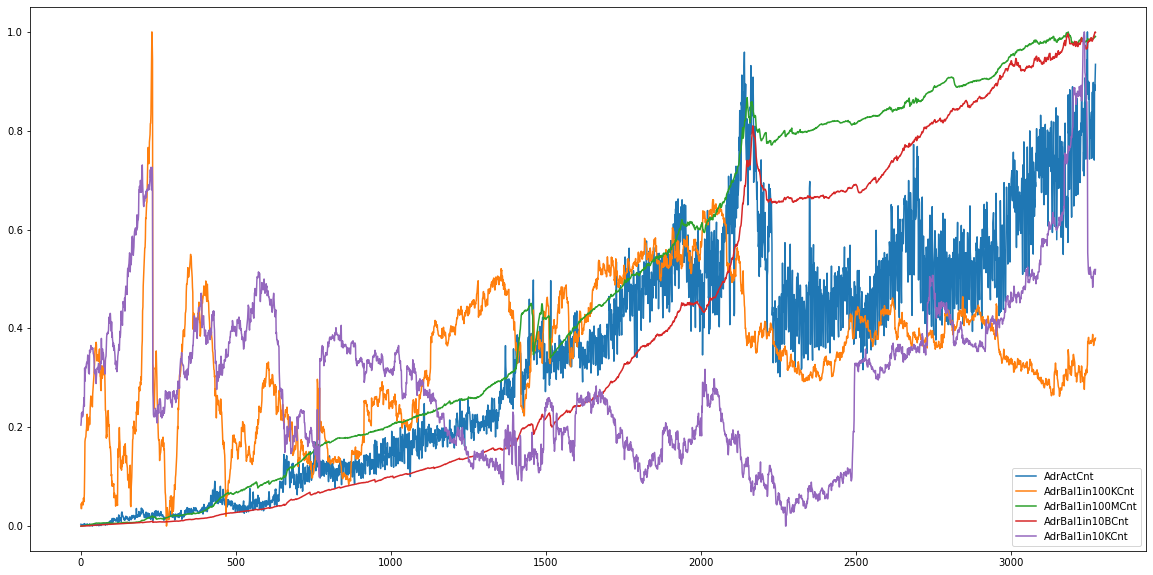
\includegraphics[scale=0.34]{Chapter5/metrics_1.png}
	\caption{Algunas métricas de la blockchain obtenidas para el análisis}
	\label{fig5}
\end{figure}

\subsection{Selección de métricas}

Antes de obtener los resultados del análisis de regresión hay que tratar con la multicolinealidad de los datos, siguiendo los pasos de \autoref{ssec:metrics} para el método VIF la correlación obtenida entre las métricas de la blockchain se muestra en la \autoref{fig6}, después de seleccionar aquellas que tuvieran una correlación mayor a $0.9$ como valor absoluto con al menos otra variable con el método de Pearson se obtuvo el subconjunto de características de la \autoref{fig7}. 

\begin{figure}[!h]
	\centering
	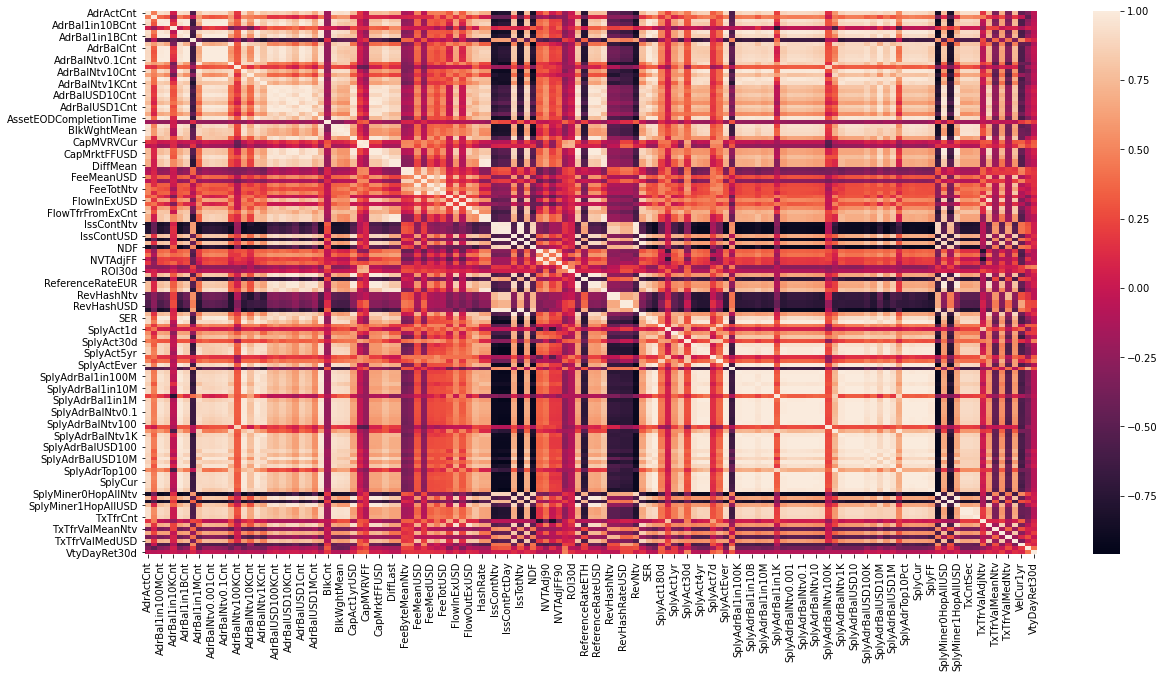
\includegraphics[scale=0.4]{Chapter5/corr_map.png}
	\caption{Correlación entre todas las métricas obtenidas}
	\label{fig6}
\end{figure}

\begin{figure}[!h]
	\centering
	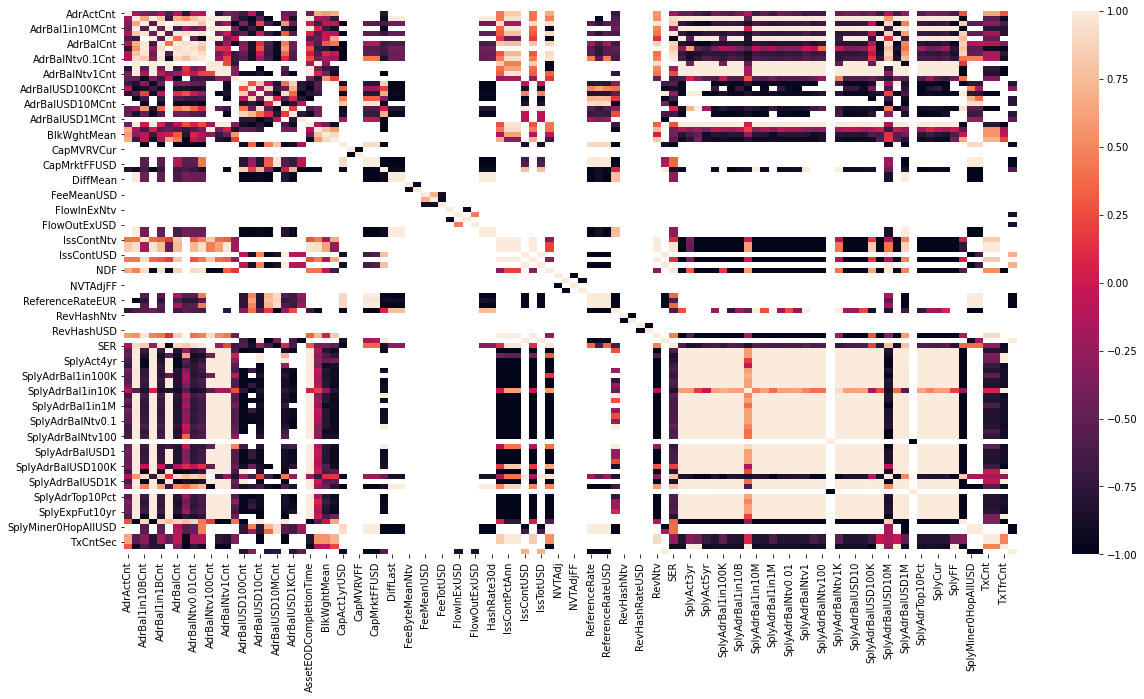
\includegraphics[scale=0.4]{Chapter5/corr_map2.png}
	\caption{Características de la blockchain con una correlación como valor absoluto mayor a 0.9}
	\label{fig7}
\end{figure}

Con las características obtenidas se calcula el VIF de las mismas como se muestra en la figura \autoref{subfig1}. La métrica con mayor multicolinealidad en los datos fue RevHashNtv mostrando mayor dependencia lineal en el supuesto de independencia. Esta variable es descartada y el VIF se calcula nuevamente. Se repite el proceso hasta obtener la tabla final de la figura \autoref{subfig2}, que son los datos a utilizar junto con aquellos que tienen poca correlación entre sí.

\begin{figure}[!h]
	\centering
	\subfloat[VIF con todas las métricas seleccionadas]
	{
		\label{subfig1}
		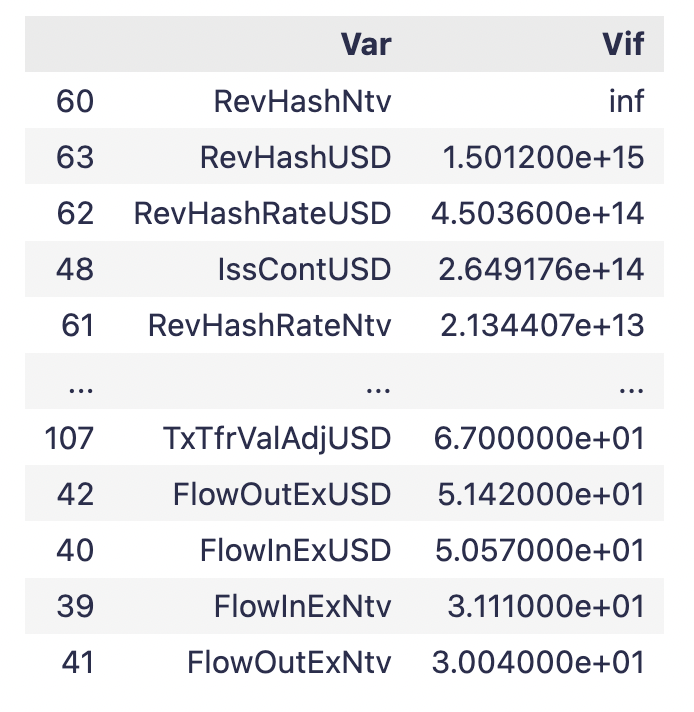
\includegraphics[width=0.45\columnwidth]{Chapter5/VIF.png}
	}
	\qquad
	\subfloat[Caracteristicas con VIF menor a cinco]
	{
		\label{subfig2}
		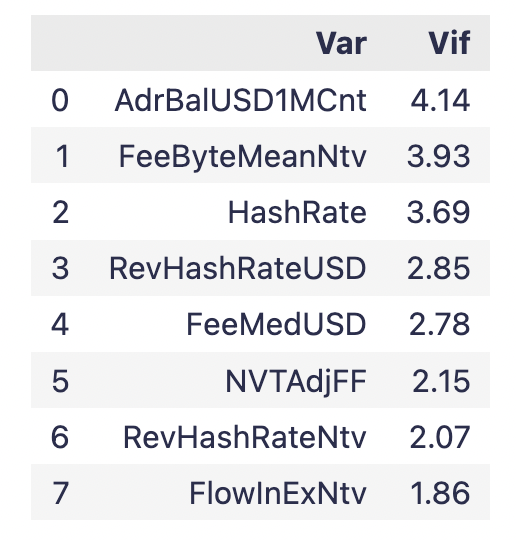
\includegraphics[width=0.45\columnwidth]{Chapter5/VIF2.png}
	}
	\caption{Tabla inicial y final después de aplicar el método VIF para eliminar multicolinealidad en los datos}
	\label{fig8}
\end{figure}

El análisis de regresión utilizando mínimos cuadrados ordinarios da la información mostrada en la \autoref{fig10}. Se puede ver que las variables con mayor peso en la predicción por el valor de sus coeficientes son \textit{AdrBalUSD1MCnt} y \textit{HashRate}.
Filtrando estas variables por su significación estadística se obtienen las características mostradas en la \autoref{fig11}. Estas variables son usadas en el análisis de componentes principales.


Los componentes principales de los datos con valores atípicos y sin valores atípicos se muestran en la \autoref{fig12} y \autoref{fig13} respectivamente. Se puede ver como hay una reducción en el número de puntos fuera del dominio de aplicabilidad (área verde), y como la gran mayoría de puntos se ajusta mejor dentro de los límites del mismo en los datos sin valores atípicos multivariados. El propósito del dominio de aplicabilidad es definir las fronteras donde el modelo puede ser utilizado y ofrecer predicciones confiables \parencite{karApplicabilityDomainStep2018}.

\begin{figure}
	\centering
	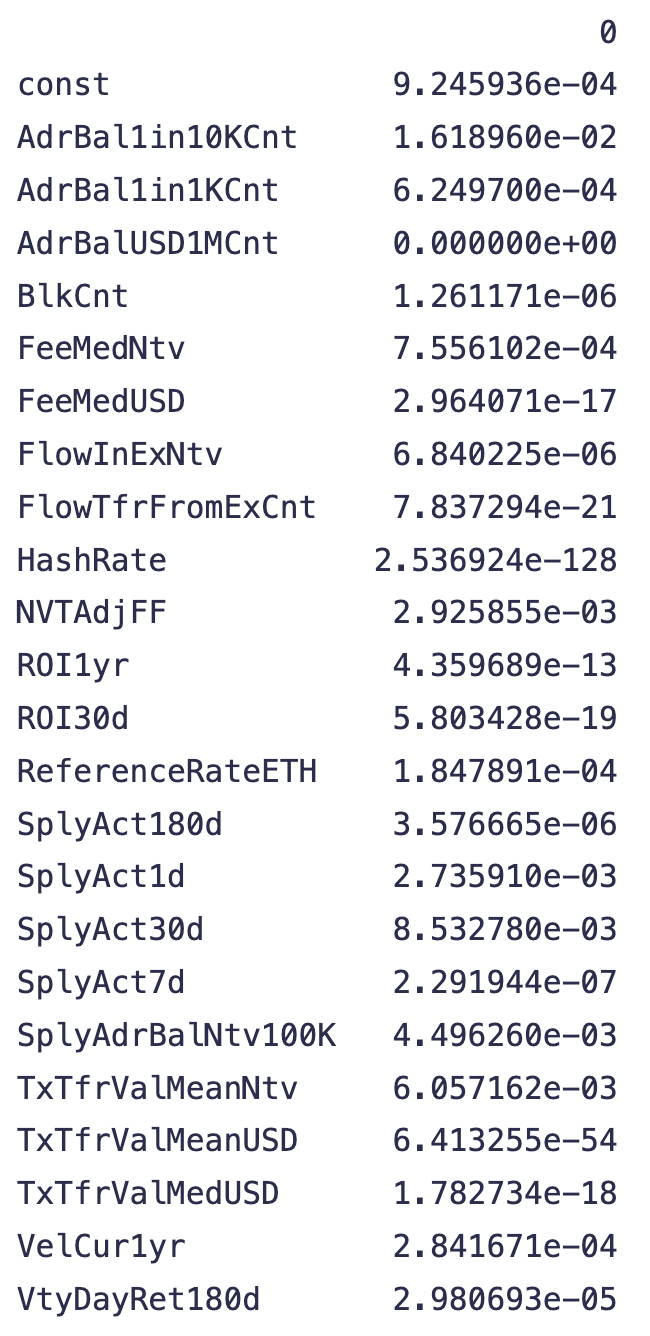
\includegraphics[scale=0.5]{Chapter5/p-val.png}
	\caption{Variables con valor p menor que 0.05}
	\label{fig11}
\end{figure}

\begin{figure}
	\centering
	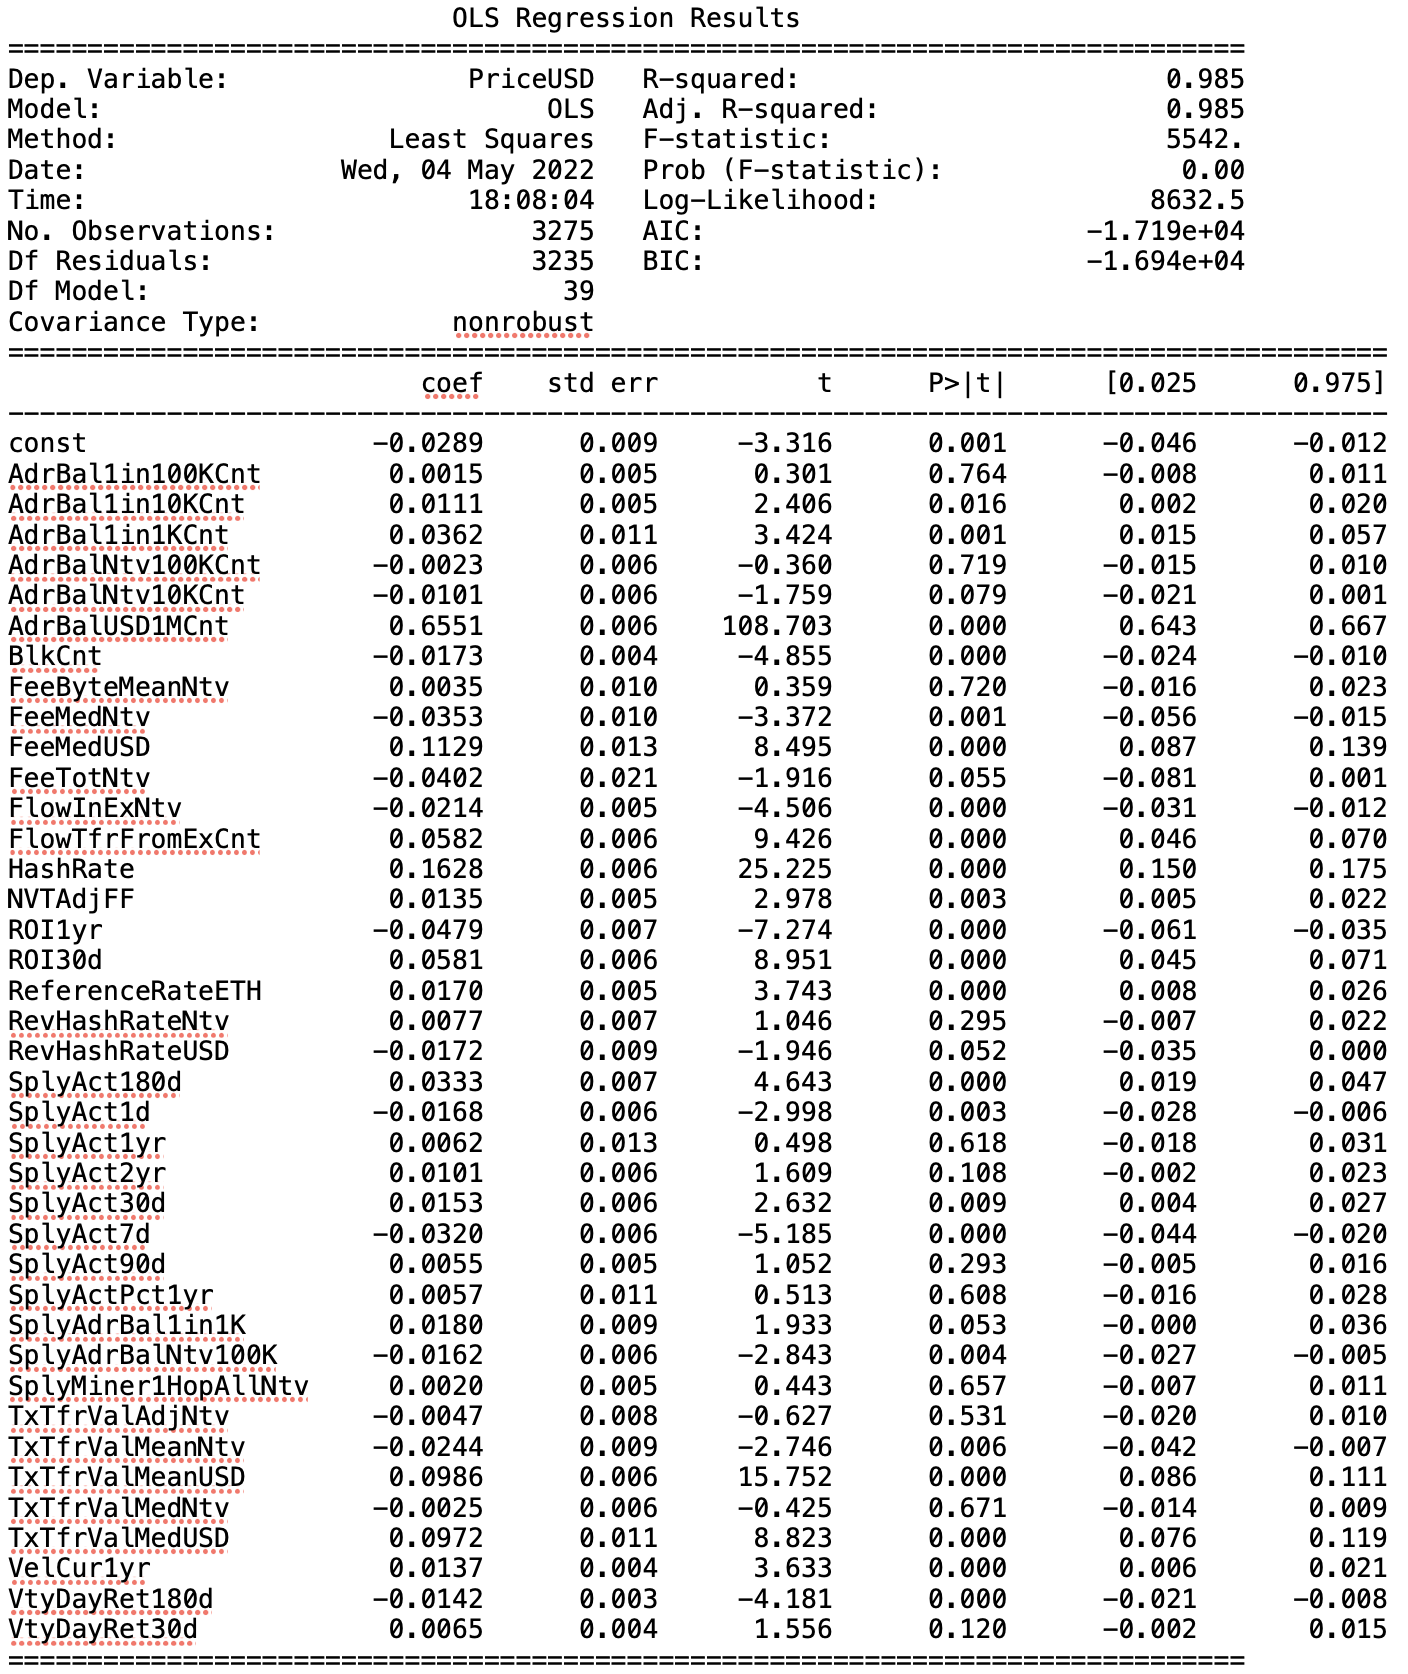
\includegraphics[scale=0.7]{Chapter5/OLS.png}
	\caption{Resultados del análisis de regresión}
	\label{fig10}
\end{figure}

\begin{figure}
	\centering
	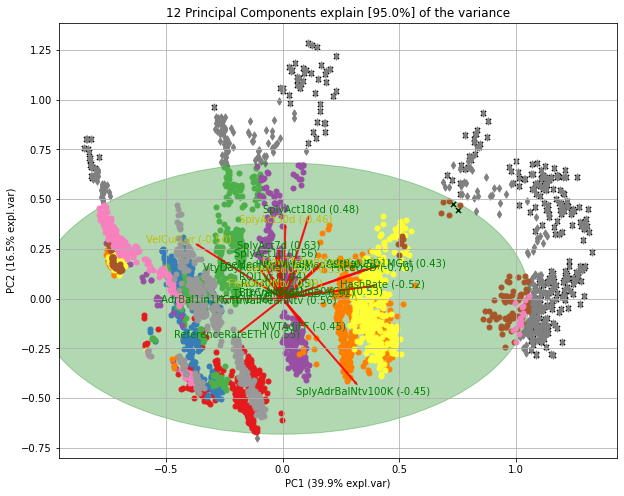
\includegraphics[scale=0.6]{Chapter5/pca_val_atipi.png}
	\caption{Componentes principales con valores atípicos multivariados}
	\label{fig12}
\end{figure}

\begin{figure}
	\centering
	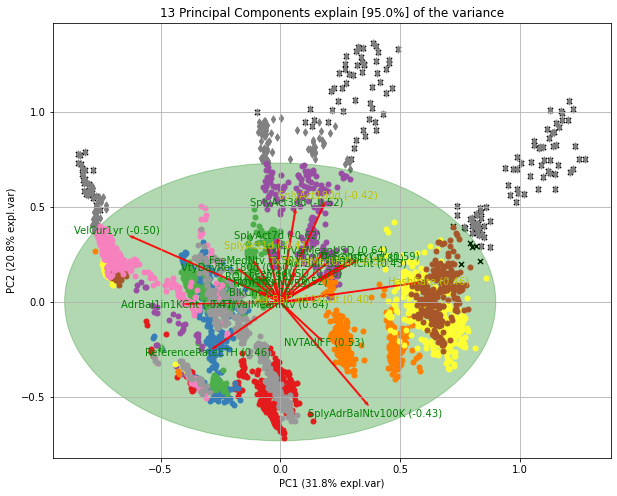
\includegraphics[scale=0.6]{Chapter5/pca_sin_va_atipi.png}
	\caption{Componentes principales sin valores atípicos multivariados}
	\label{fig13}
\end{figure}

Entonces, seleccionando aquellas variables que tienen la misma dirección y mayor o igual magnitud que el precio se obtienen los componentes principales de la \autoref{fig14}. Estas variables son: \textit{HashRate}, \textit{SplyAct180d} y \textit{SplyAct30d}. 

Realizando un dendrograma de correlación con las variables obtenidas se observa que el precio y hashrate pertenecen al mismo grupo, significando esto que es la variable que más afecta en la varianza del precio y que además está altamente correlacionada con el mismo. \textit{Hashrate} es la velocidad media a la que los mineros resuelven hashes durante el día. La velocidad del hash es la velocidad a la que se completan los cálculos de todos los mineros de la red. Esta velocidad se deriva de la dificultad de minado y de la velocidad en la que el bloque fue emitido. 

\begin{figure}
	\centering
	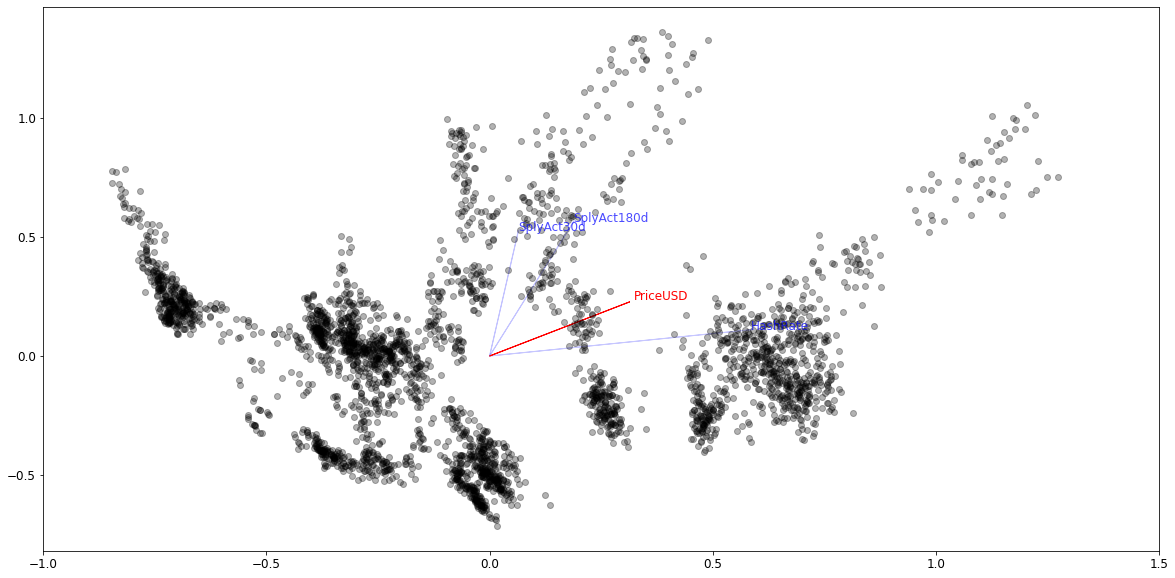
\includegraphics[scale=0.4]{Chapter5/pca_price.png}
	\caption{Métricas obtenidas que influye en la varianza del precio}
	\label{fig14}
\end{figure}

\begin{figure}
	\centering
	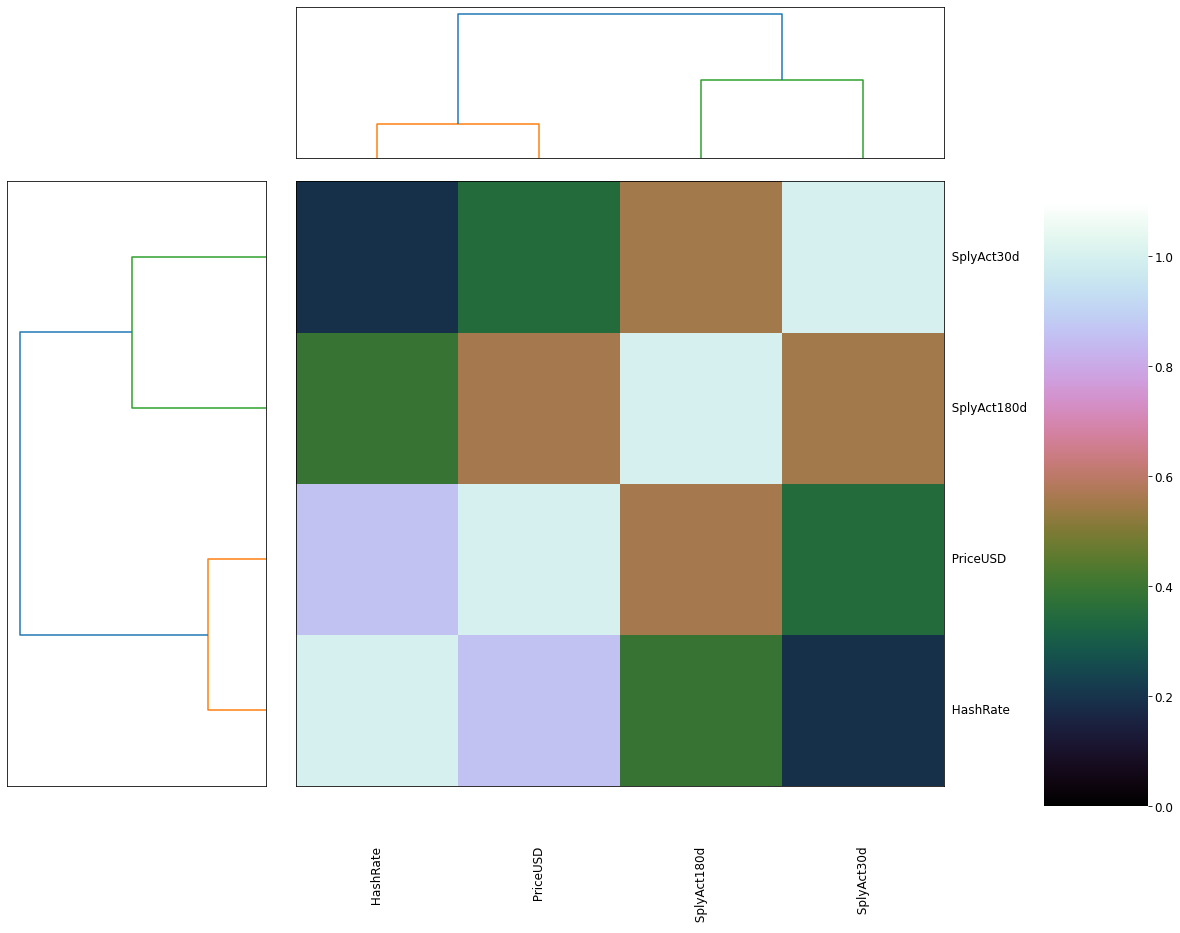
\includegraphics[scale=0.3]{Chapter5/dendo.png}
	\caption{Dendrograma de correlación con las métricas obtenidas por el PCA}
	\label{fig15}
\end{figure}

\section{Predicción del precio}

\subsection{Datos y pre-procesamiento}
Los datos descargados y procesados en formato OHLCV tienen la estructura mostrada en \autoref{fig16}, después de realizar el análisis de métricas de la blockchain detallado en la \autoref{Metodologia} se llega al conjunto de datos final mostrado en la \autoref{fig17}.

\begin{figure}[h!]
	\centering
	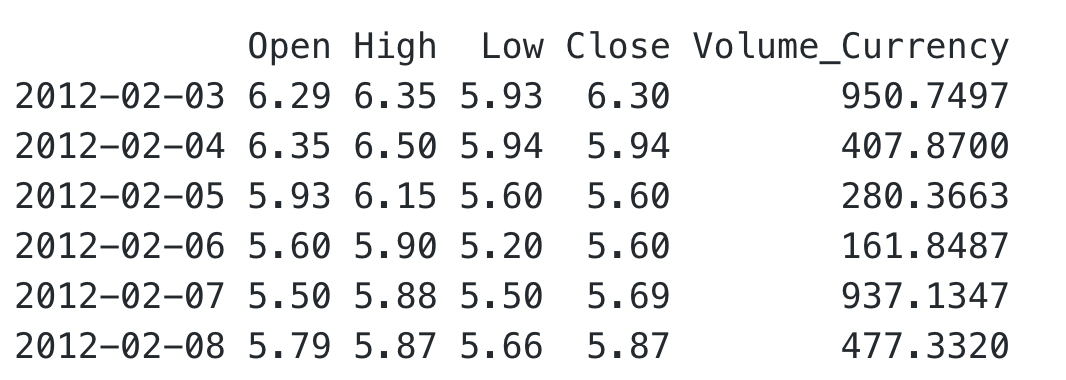
\includegraphics[scale=0.5]{Chapter5/ohlcv.png}
	\caption{Características financieras en formato OHLCV}
	\label{fig16}
\end{figure}

\begin{figure}[h!]
	\centering
	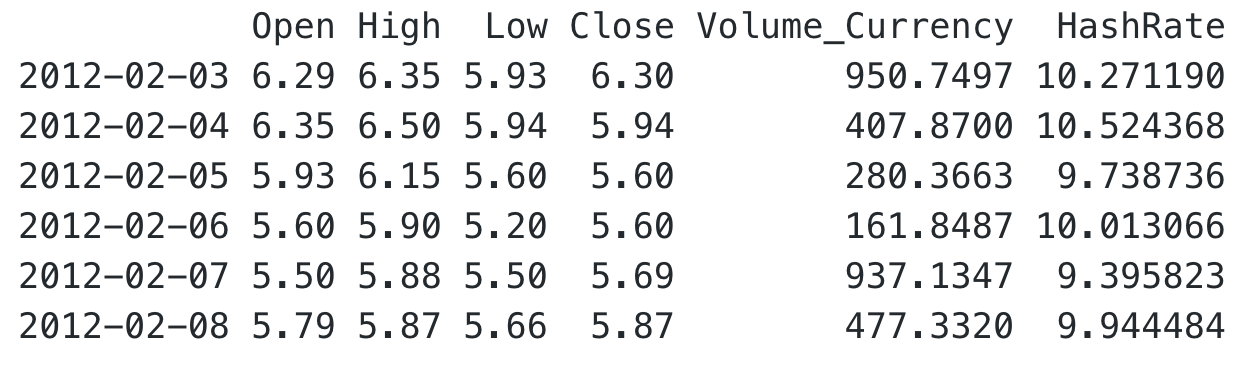
\includegraphics[scale=0.5]{Chapter5/ohlcv_complete.png}
	\caption{Conjunto de datos final con la métrica obtenida por el análisis de la blockchain}
	\label{fig17}
\end{figure}

La volatilidad del precio de cierre del activo se muestra en la \autoref{fig18}. En esta se puede ver como a partir del 2017 el precio empieza a despegar de forma exponencial, llegando a valer en 2018 casi \$20,000 dólares y a su vez ocurriendo su primer crac debido a la salida y poco apoyo de grandes financieros como Goldman Sachs o a la división de la comunidad creando un fork con una nueva visión de la moneda \parencite{peterssonWhyBitcoinCrashed2018}. Sea como fuere, la criptomoneda comenzó una etapa lenta de recuperación con caídas de por medio como la de 2019 o 2020 debido a sanciones de grandes países como China, aun así, desde finales de 2020 el precio ha vuelto a su crecimiento exponencial debido a la aceptación de cada vez más empresas y el público en general pero manteniendo su gran volatilidad. Actualmente, a inicios de mayo de 2022, el precio ronda aproximadamente los \$40,000 dólares manteniendo cierta estabilidad a pesar de la crisis económica causada por la COVID-19 y la invasión de Rusia a Ucrania.

\begin{figure}[h!]
	\centering
	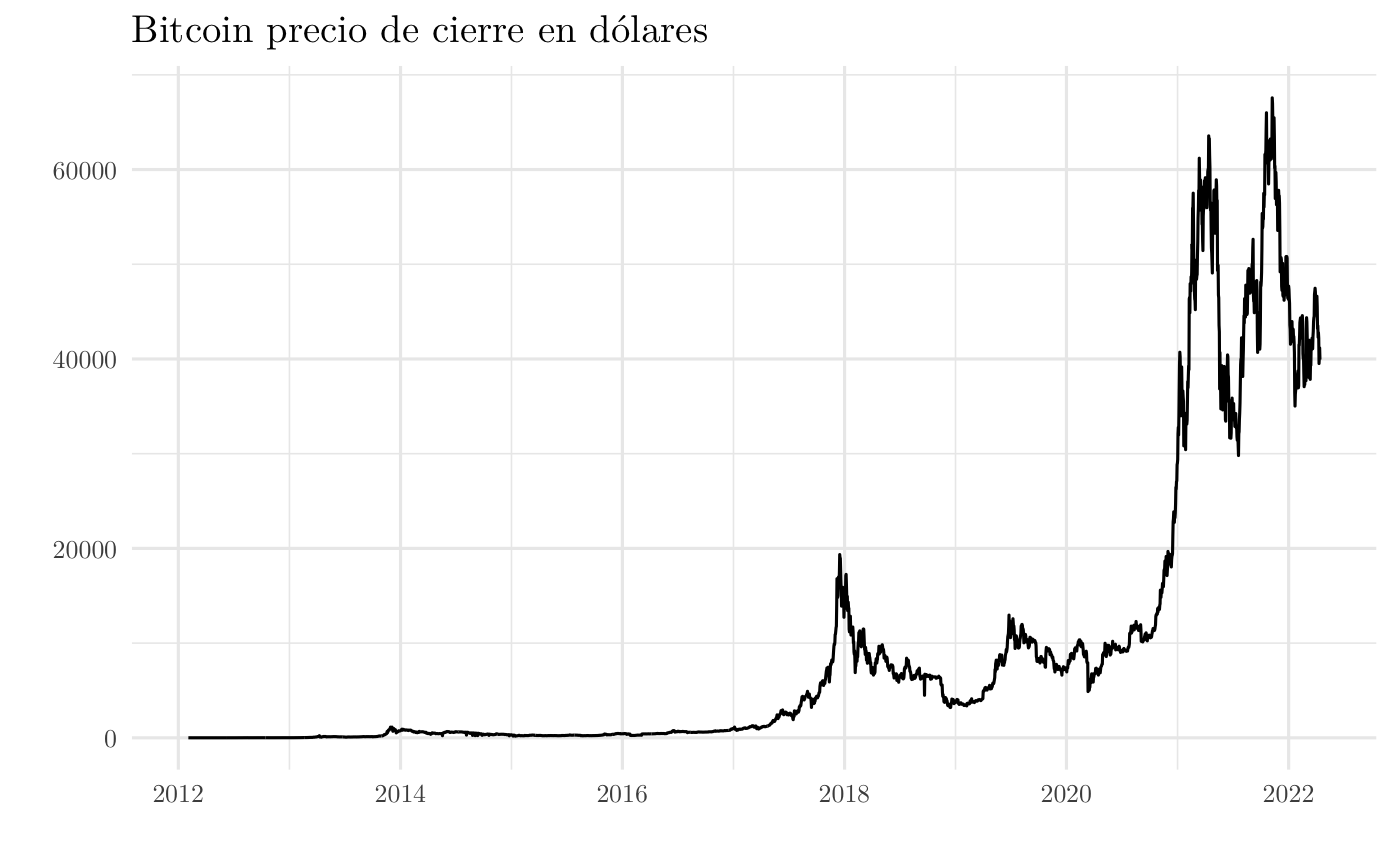
\includegraphics[scale=0.35]{Chapter5/btc_price.png}
	\caption{Serie de tiempo del precio del bitcoin en dólares}
	\label{fig18}
\end{figure}

\subsection{Selección de modelo}

La correlación entre las variables financieras se muestra en la \autoref{fig19}, donde se puede observar que todas las características cuentan con una correlación muy alta y por lo tanto todas son tomadas en cuenta para el análisis de precio. Estas variables son transformadas como se muestra en la \autoref{met:prediccion}. Los resultados se pueden observar en la \autoref{fig20}. 

\begin{figure}[h!]
	\centering
	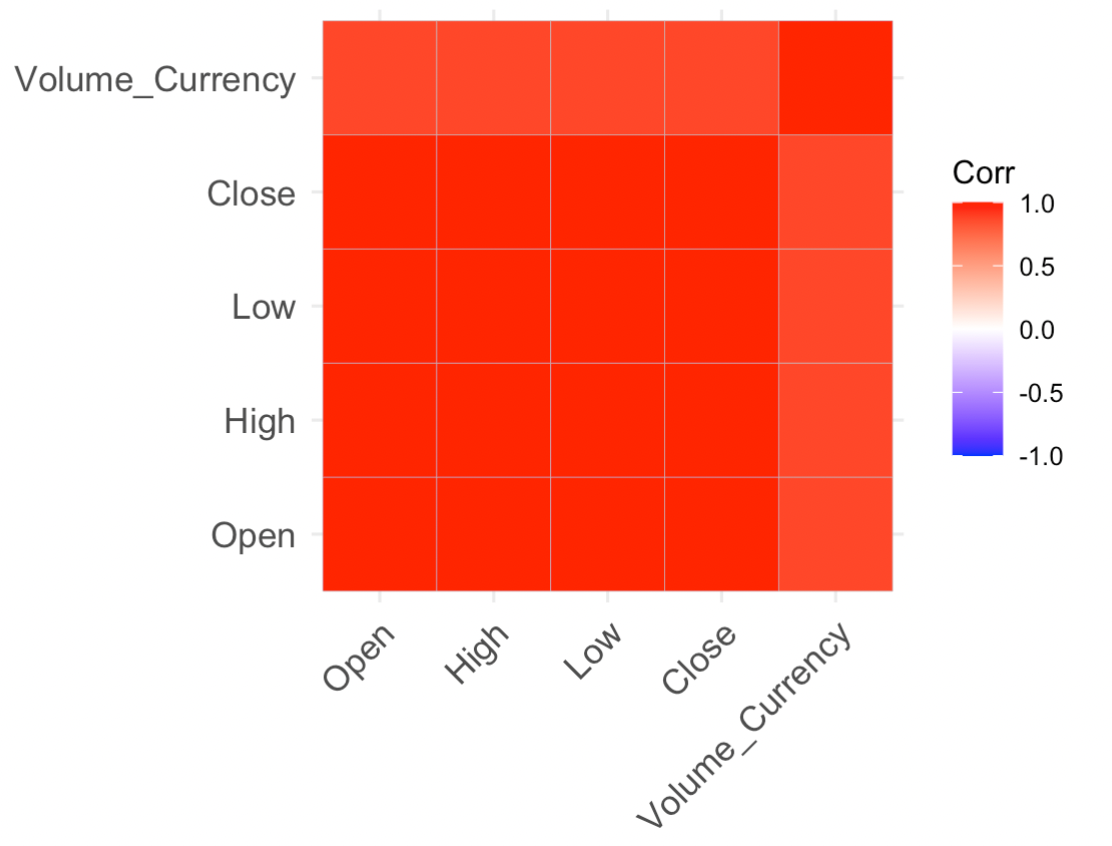
\includegraphics[scale=0.5]{Chapter5/finance_corr.png}
	\caption{Correlación entre métricas financieras}
	\label{fig19}
\end{figure}

\begin{figure}[!h]
	\centering
	\subfloat[Transformación logaritmica]
	{
		\label{subfig3}
		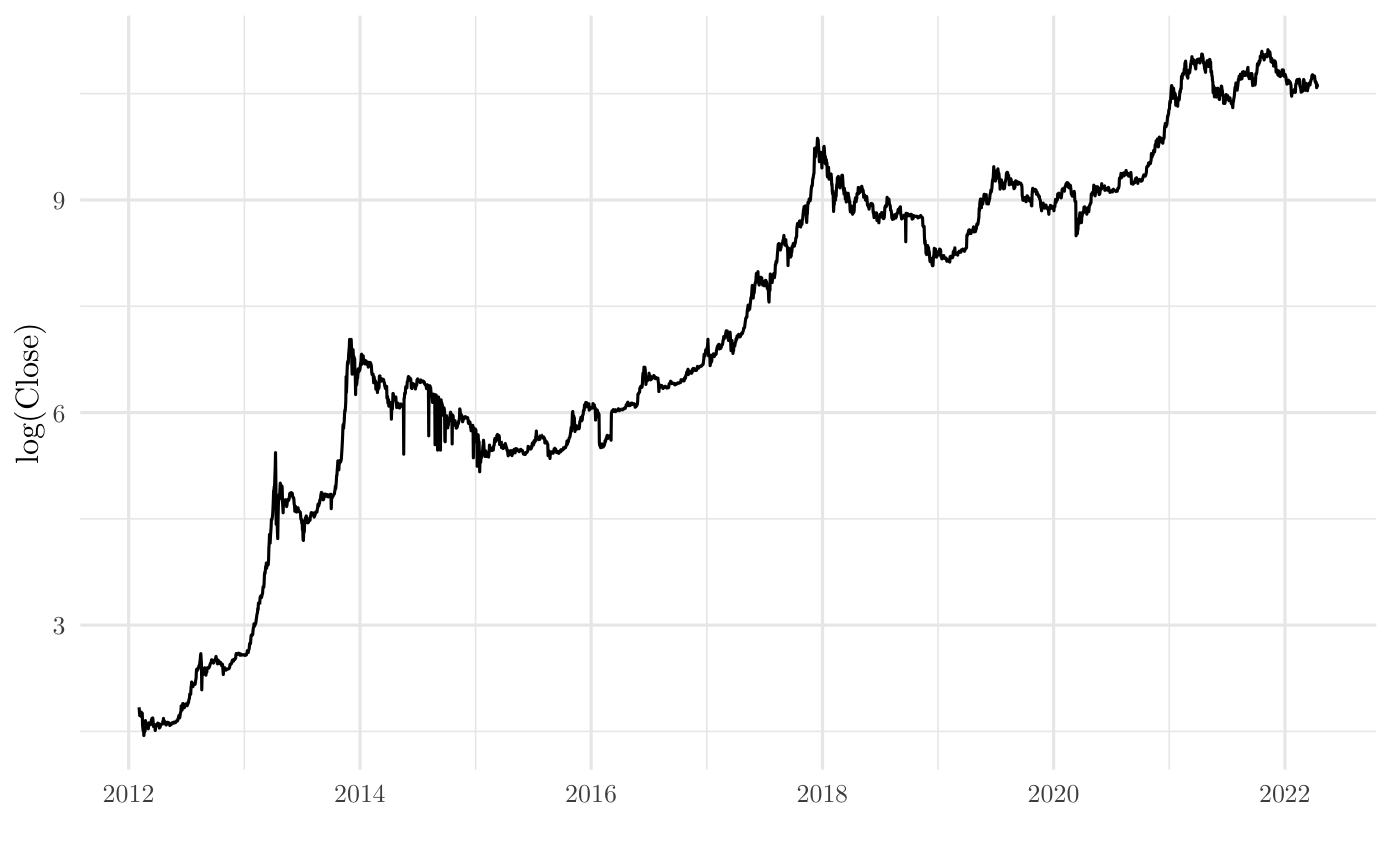
\includegraphics[width=0.45\columnwidth]{Chapter5/log_close.png}
	}
	\qquad
	\subfloat[Transformación BoxCox]
	{
		\label{subfig4}
		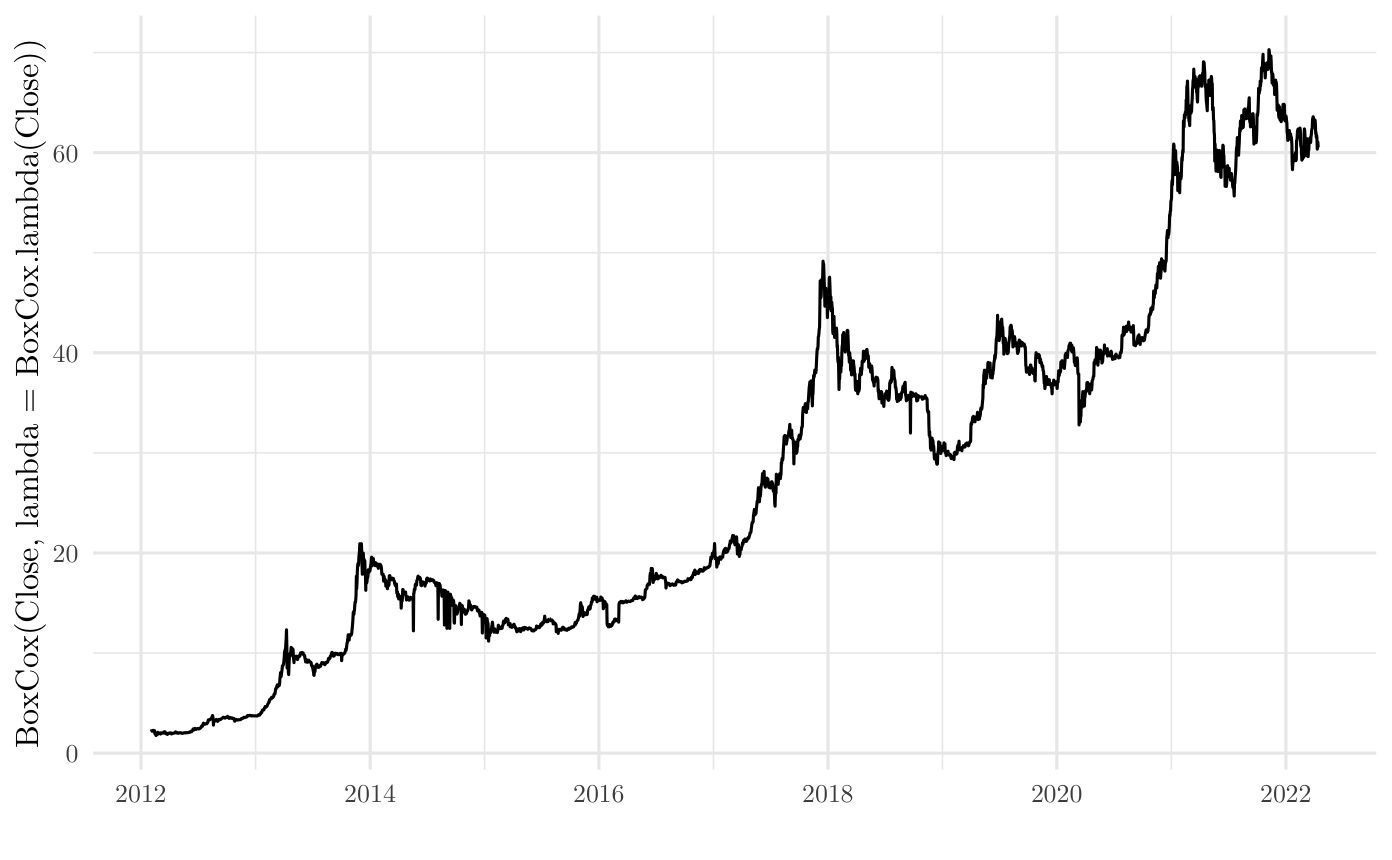
\includegraphics[width=0.45\columnwidth]{Chapter5/boxcox_close.png}
	}
	\qquad
	\subfloat[Retornos diarios del precio]
	{
		\label{subfig5}
		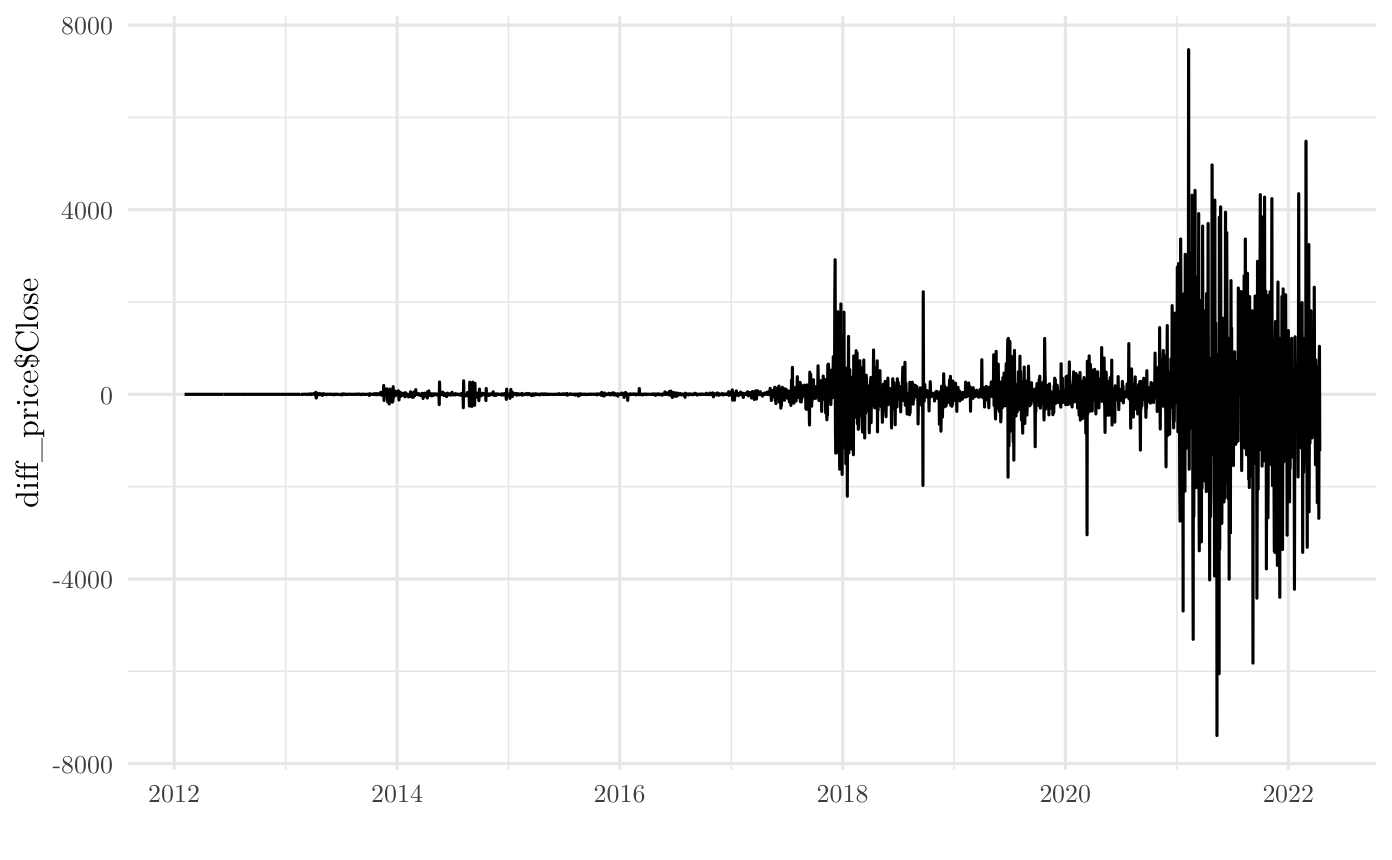
\includegraphics[width=0.45\columnwidth]{Chapter5/diff_close.png}
	}
	\qquad
	\subfloat[Retornos logaritmicos del precio]
	{
		\label{subfig6}
		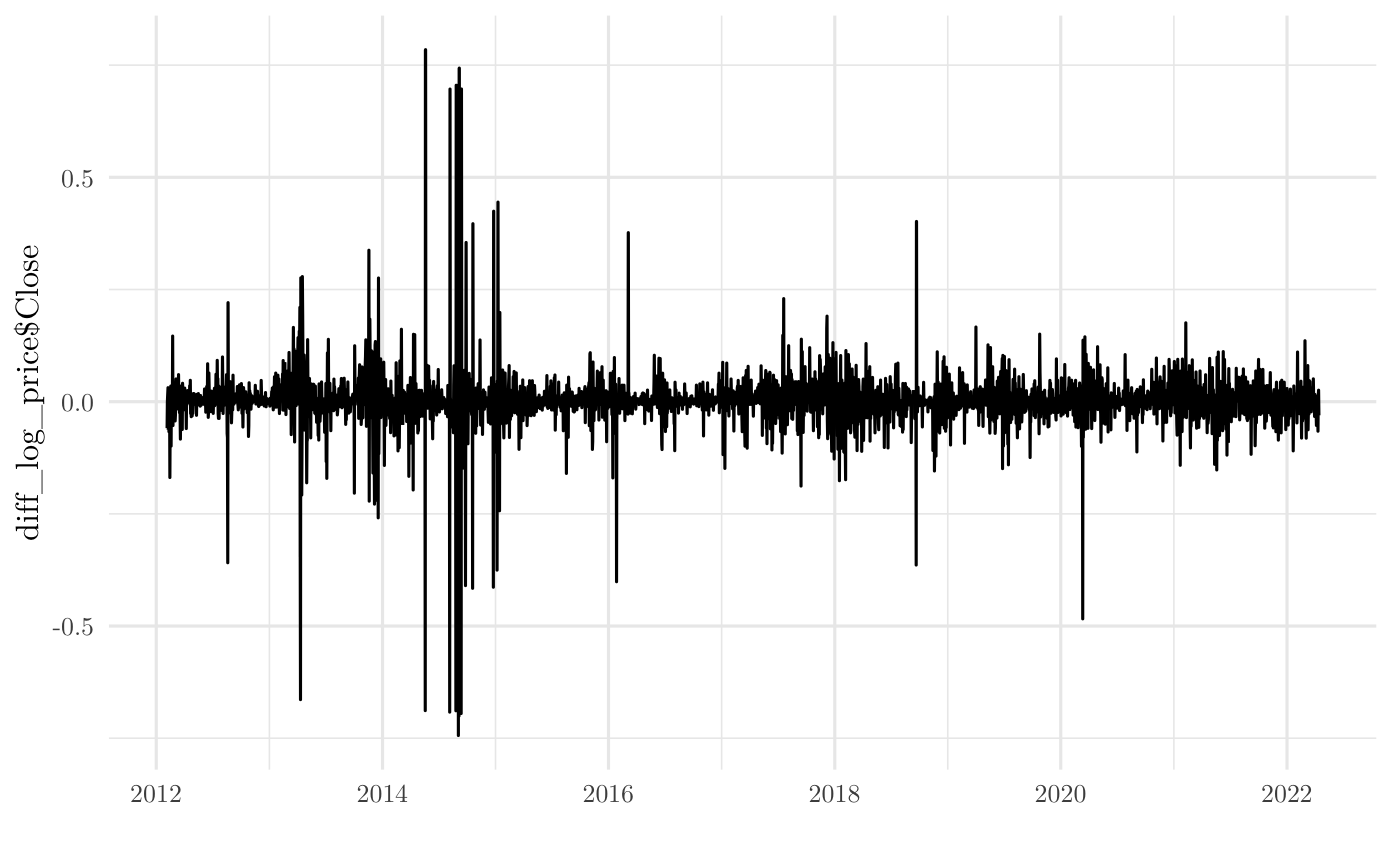
\includegraphics[width=0.45\columnwidth]{Chapter5/diff_log_price.png}
	}
	\caption{Transformaciones matemáticas aplicadas a los datos}
	\label{fig20}
\end{figure}

El parámetro lambda encontrado que mejor estabiliza la varianza en la transformación BoxCox es $\lambda = 0.2689427$, aunque la transformación logaritmica muestra una mejor tendencia a simple vista, por otro lado, las diferencias del precio muestran que en los últimos años han habido mayores rendimientos, sin embargo, si la comparamos con las diferencias logarítmicas el porcentaje de rendimientos no es mayor que el de finales del 2014. 

Después de entrenar los datos transformados con los distintos modelos seleccionados y calculando sus indicadores de error y exactitud, se elabora la \autoref{tab:Table4}. Se observa que el modelo con el menor indice de error y exactitud es Random Forest alcanzando un error de \$38.63 dólares.
En la \autoref{fig21} se pude ver la predicción sobre el conjunto de datos de prueba, los puntos negros son los datos originales y la linea roja los datos predichos. Si se realiza el mismo ejercicio sobre únicamente las características financieras con el modelo RF se alcanza un error de \$56.77 dólares, mostrándose que agregando esta única característica puede mejorar la predicción hasta \$18.14 dólares.
 
\begin{table}
	\centering
	\begin{adjustbox}{width=0.83\textwidth}
	\begin{tabular}{m{5cm} m{3.5cm} m{3cm} m{3cm} }
		\toprule
		\textbf{Transformación} & \textbf{Modelo} & \textbf{RMSE} & \textbf{Theil’s U}\\
		\midrule
		Original&Naive & 237.2850  & 0.05137089\\
		&SES   & 237.2542  & 0.05136421\\
		&Holt  & 237.2228  & 0.05135741\\
		&ETS   & 255.9911  & 0.05542065\\
		&ARIMA & 237.2850  & 0.05137089\\
		&RTS   & 82.86021   & 0.01793877\\
		&SVM   & 142.1834   & 0.03078192\\
		&RF    & \textbf{39.38410}   & \textbf{0.00852643}\\
		&LSTM  & 1.40e+07  & 3049.5840\\ \\
		log	&Naive & 2.372850  & 0.05137089\\
		&SES   & 246.9256  & 0.05345801\\
		&Holt  & 247.6223  & 0.05360884\\
		&ETS   & 247.6223  & 0.05360884\\
		&ARIMA & 247.7399 & 0.05363431\\
		&RTS   & 89.22367   & 0.01931643\\
		&SVM   & 385.0302   & 0.08335690\\
		&RF    & \textbf{38.62311}   & \textbf{0.00836168}\\
		&LSTM  & 2.74e+14  & 5.938e+10\\ \\
		BoxCox	&Naive & 2.372850  & 0.05137089\\
		&SES   & 242.2361  & 0.05244277\\
		&Holt  & 242.3319  & 0.05246350\\
		&ETS   & 250.4998  & 0.05423181\\
		&ARIMA & 242.7126 & 0.05254592\\
		&RTS   & 85.04896   & 0.01841263\\
		&SVM   & 183.3686   & 0.03969827\\
		&RF    & \textbf{38.73046}   & \textbf{0.00838493}\\
		&LSTM  & 2.43e+09  & 52683.350\\ \\
		diff		&Naive & 336.2168  	& 0.07278906\\
		&SES   & 237.2766  	& 0.05136907\\
		&Holt  & 237.2176  	& 0.05135629\\
		&ETS   & 237.2766 	& 0.05136907\\
		&ARIMA & 237.2852  	& 0.05137092\\
		&RTS   & 317.0049   & 0.06862979\\
		&SVM   & 328.3989   & 0.07109653\\
		&RF    & 320.6893	& 0.06942740\\
		&LSTM  & 27824.87  	& 6.02393013\\ \\
		diff(log)	&Naive & 237.2976  	& 0.05137361\\
		&SES   & 237.2964  	& 0.05137335\\
		&Holt  & 237.2964  	& 0.05137335\\
		&ETS   & 237.2964  	& 0.05137335\\
		&ARIMA & 237.2960 	& 0.05137327\\
		&RTS   & 237.2942  	& 0.05137287\\
		&SVM   & 237.2944  	& 0.05137291\\
		&RF    & 237.2939  	& 0.05137281\\
		&LSTM  & 237.2968	& 0.05137345\\
		\bottomrule
		\hline
	\end{tabular}
	\end{adjustbox}
	\caption{Resultados de la comparación de los modelos durante la fase de entrenamiento estimando RMSE y Theil’s U.}
	\label{tab:Table4}
\end{table}  
\section{Análisis topológico de datos}

\begin{figure}
	\centering
	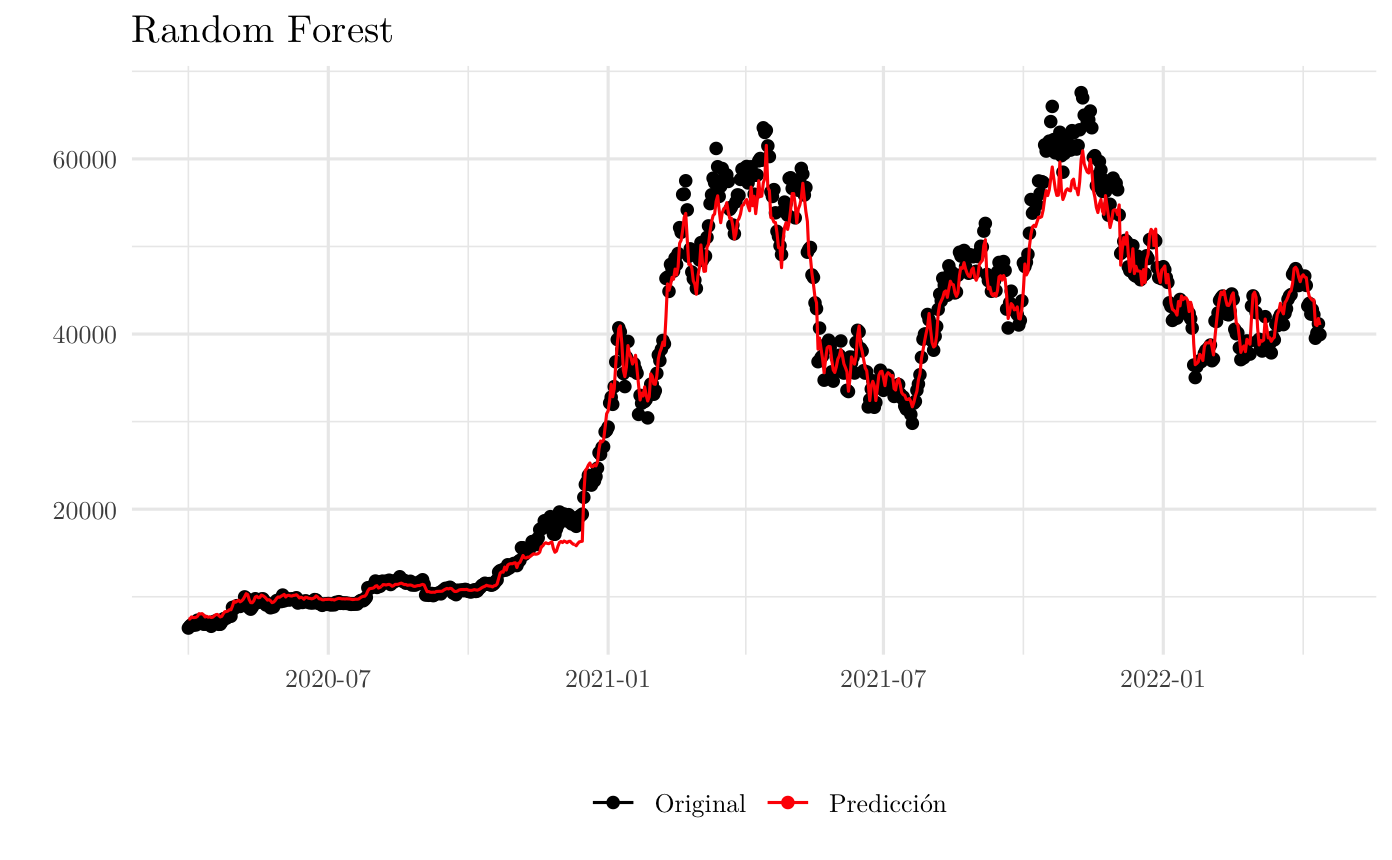
\includegraphics[scale=0.35]{Chapter5/pred_RF.png}
	\caption{Predicción sobre el conjunto de prueba}
	\label{fig21}
\end{figure}

\subsection{Norma $C^1$}

Para encontrar un crac en un periodo de tiempo especifico se recomienda segmentar la serie de tiempo en intervalos pequeños que inicien y terminen en las correspondientes caídas críticas \parencite{gideaTopologicalRecognitionCritical2020}, sin embargo, para la toma de decisiones de inversión se intentó capturar la mayor cantidad de caídas en todo el periodo establecido. Después de aplicar la metodología de la \autoref{met_tda} se obtuvieron los normas $L^1$ de los panoramas de persistencia de las nubes de datos generados con una ventana deslizante de 50 días como recomienda Guidea y col. \parencite*{gideaTopologicalRecognitionCritical2020} en su artículo. La \autoref{fig22} muestra los cambios en la forma de los datos en periodos de tiempo específicos, entonces, antes de una transición crítica los valores absolutos de las diferencias también toman valores cada vez más altos, siendo la suma de estos la norma $C^1$, que tiene la ventaja de crecer mucho en un instante de tiempo previo al actual si se acerca a un cambio rápido en la geometría de los datos. La \autoref{fig23} nos muestra los resultados de aplicar TDA al precio de cierre del bitcoin y calcular la norma $C^1$. La explicación de los picos máximos y su relación con las caídas más pronunciadas en el precio se detallaran más adelante en la \autoref{res_clasificacion}.

\begin{figure}
	\centering
	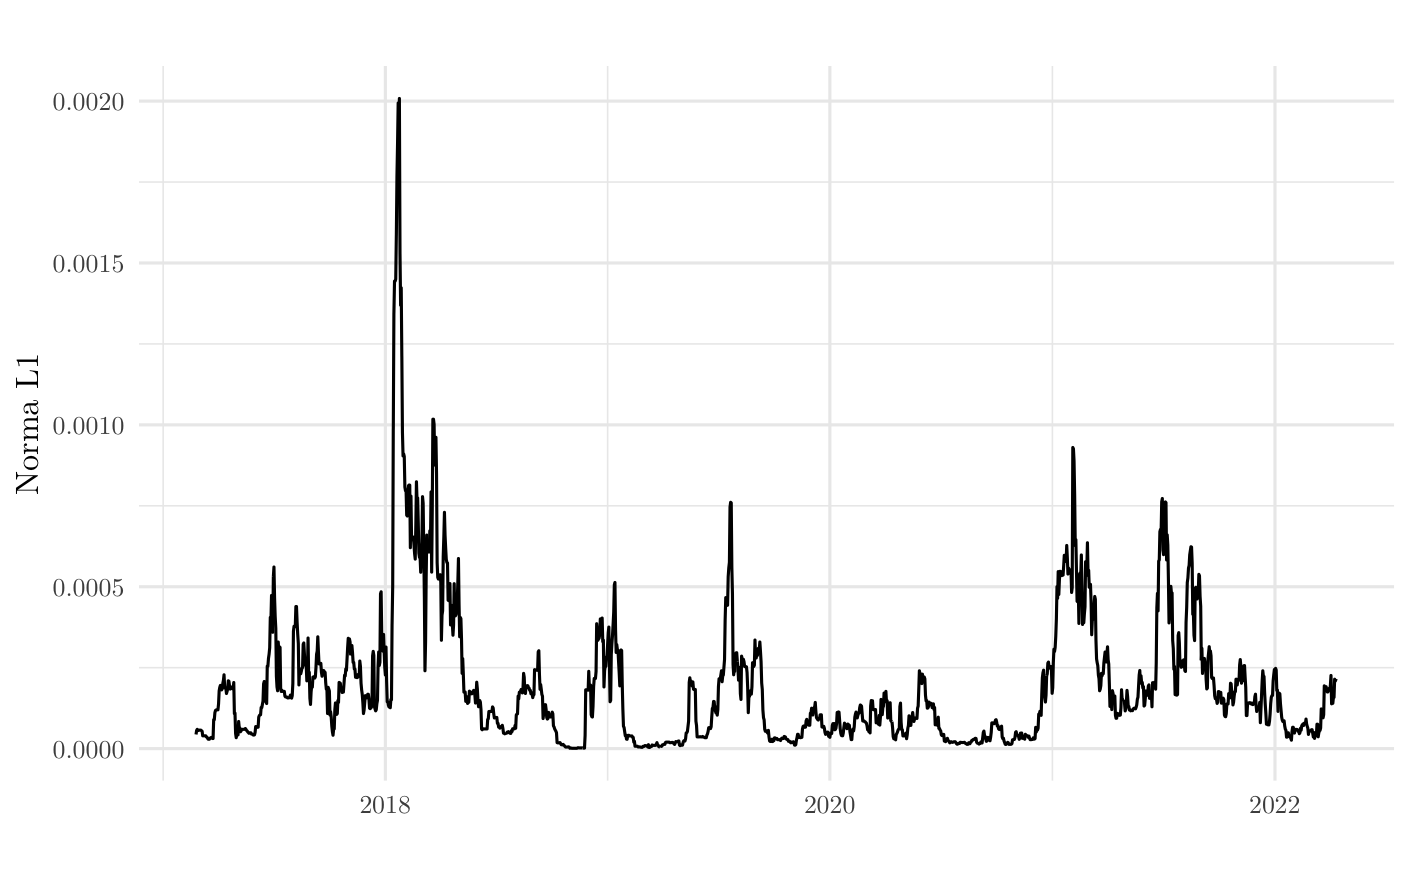
\includegraphics[scale=0.3]{Chapter5/norm_l1.png}
	\caption{Norma $L^1$ de los datos totales}
	\label{fig22}
\end{figure}

\begin{figure}
	\centering
	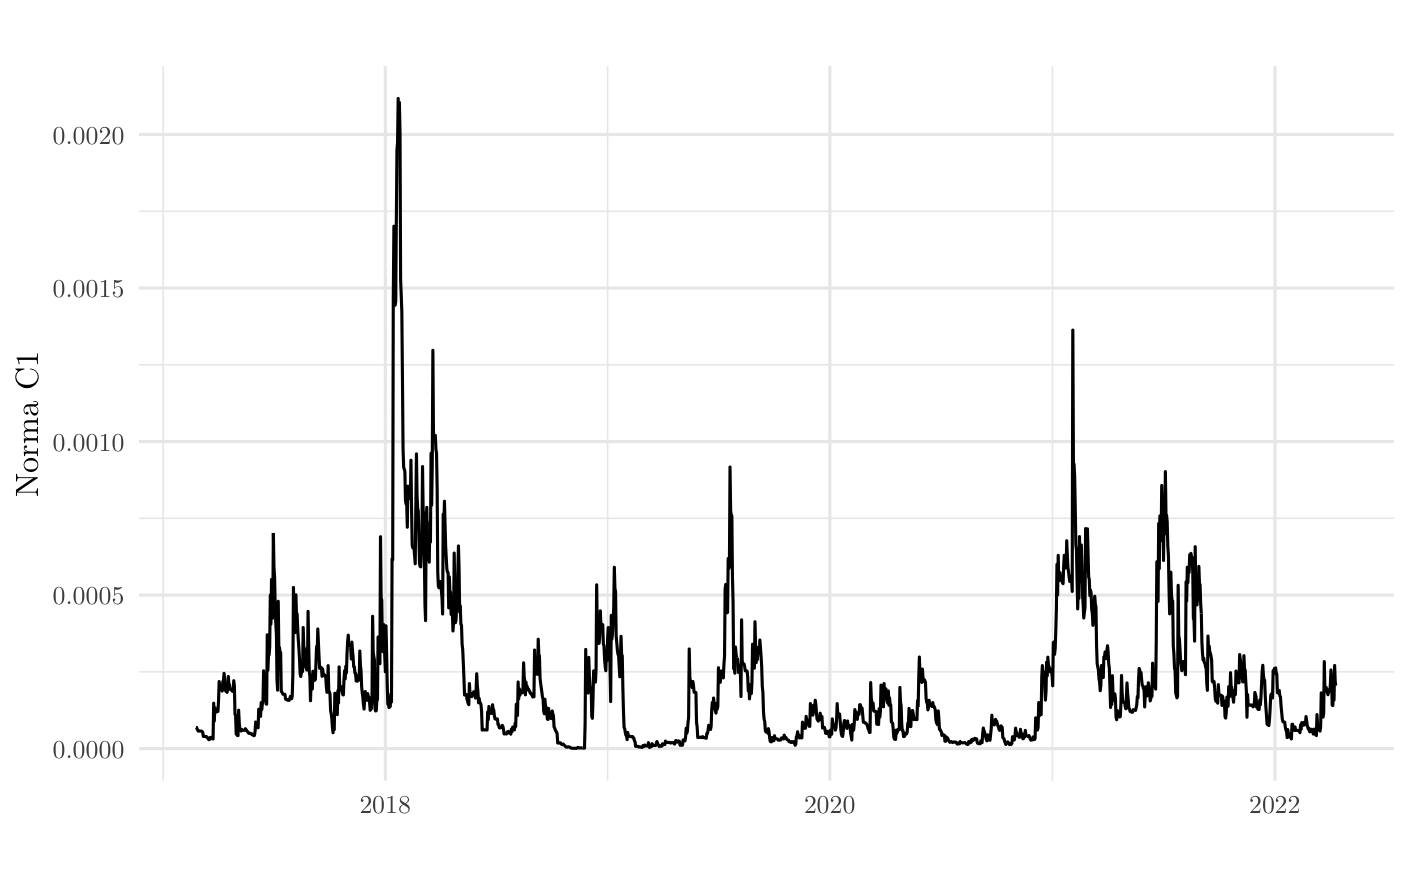
\includegraphics[scale=0.3]{Chapter5/norm_c1.png}
	\caption{Norma $C^1$ de los datos totales}
	\label{fig23}
\end{figure}

\subsection{Cluster de riesgo}

Tomando ventaja de la metodología para la detección de cracs económicos se estudian los últimos 90 días del la serie de tiempo del precio y se realiza un análisis de caídas, para ello primero se cargan los datos de los últimos tres meses y se calcula la norma $C^1$ de los datos como se muestra en la \autoref{fig24}, luego se calculan los posibles clusters de riesgo usando K-means como se explica en la \autoref{met_tda} y se selecciona el agrupamiento según los criterios antes especificados en la metodología. En este caso se obtuvieron los clusters de la \autoref{fig25} donde se puede deducir que el cluster de riesgo es el uno y se comprueba colocando el agrupamiento sobre los datos originales como en la \autoref{fig26}. Esto se realiza de forma automática y será de ayuda para complementar la toma de decisiones de inversión de la sección siguiente.

\begin{figure}
	\centering
	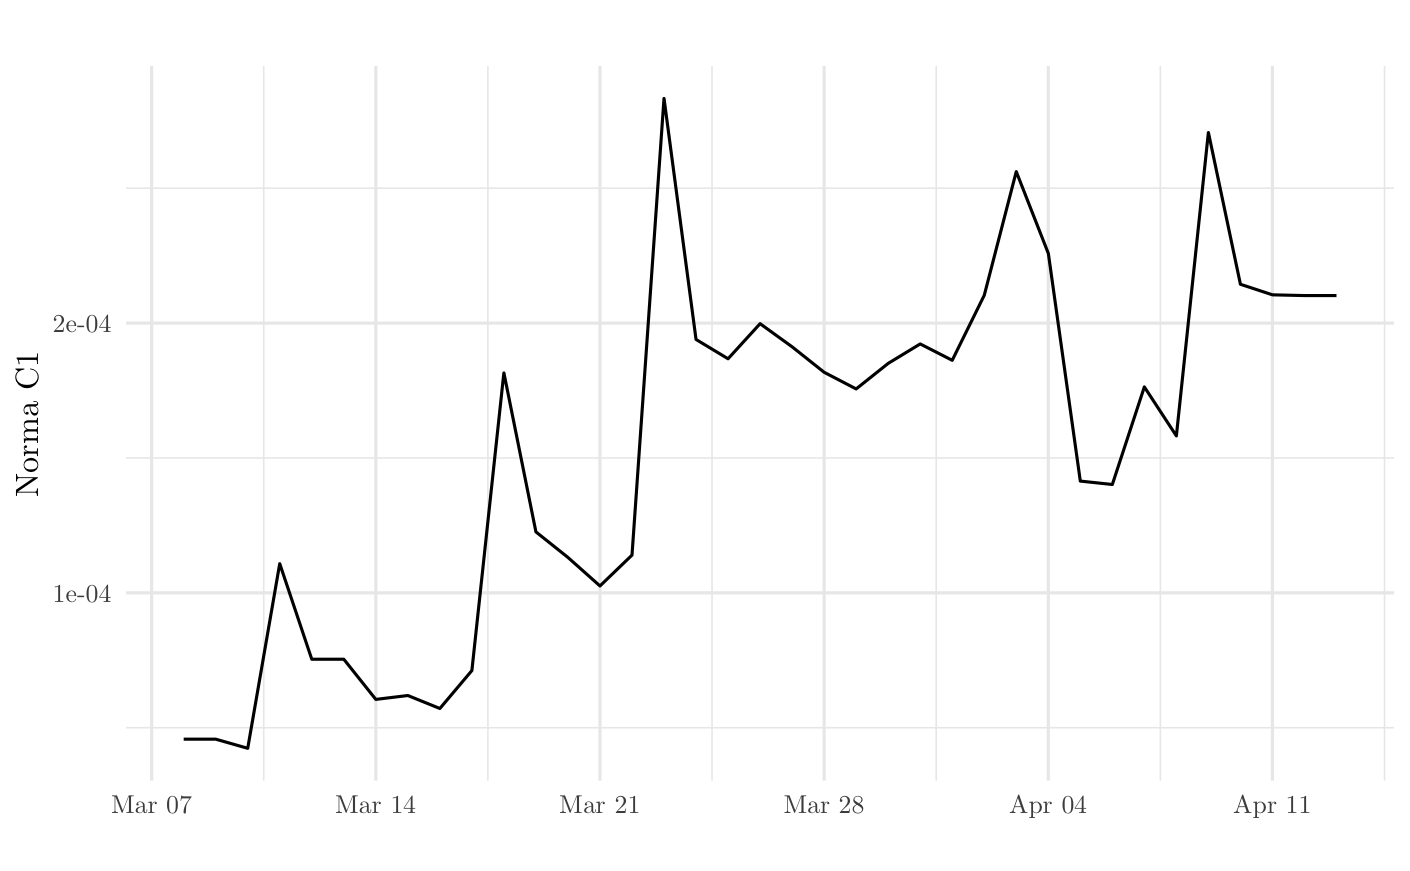
\includegraphics[scale=0.3]{Chapter5/norma_c1_3meses.png}
	\caption{Norma $C^1$ desde enero hasta abril de 2022}
	\label{fig24}
\end{figure}

\begin{figure}[h!]
	\centering
	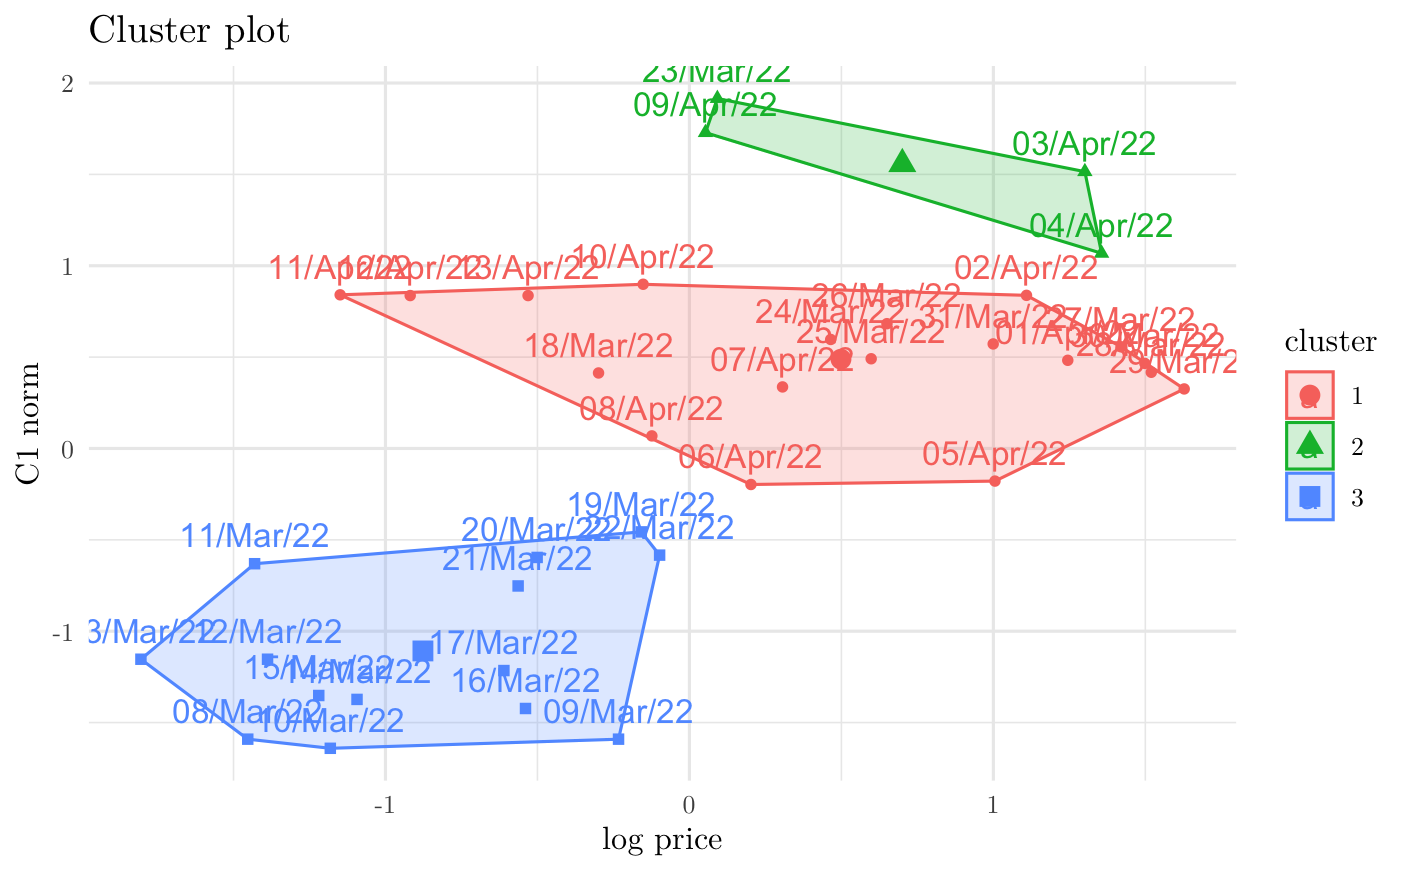
\includegraphics[scale=0.3]{Chapter5/cluster_riesgo.png}
	\caption{Agrupamientos generados usando K-means para detectar el cluster de riesgo de caídas}
	\label{fig25}
\end{figure}

\begin{figure}[h!]
	\centering
	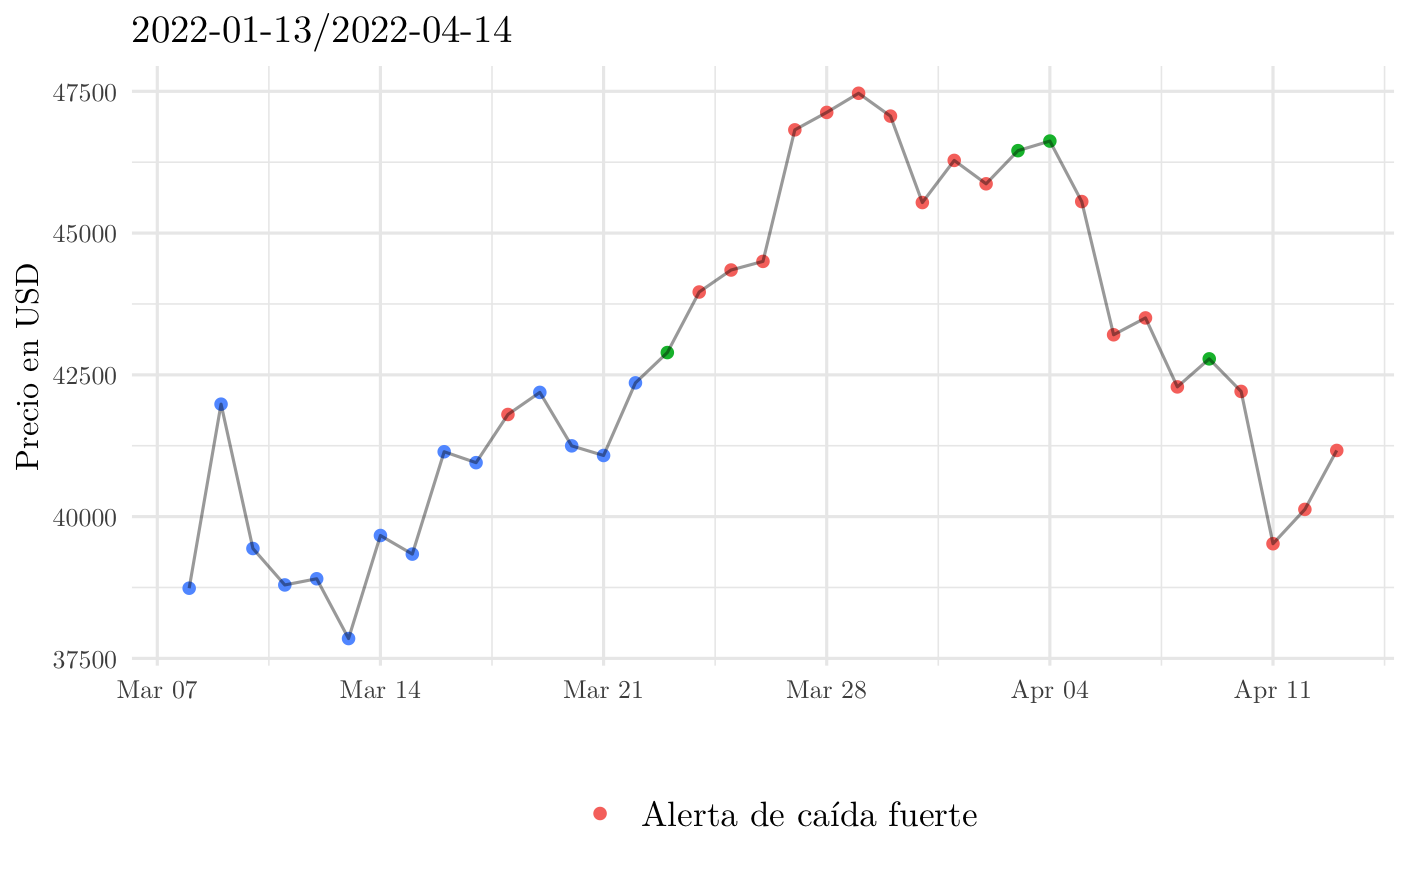
\includegraphics[scale=0.3]{Chapter5/pred_TDA.png}
	\caption{Cluster de riesgo sobre datos del precio originales}
	\label{fig26}
\end{figure}


\section{Clasificación}
\label{res_clasificacion}

\subsection{Transformaciones}
Ya que los datos utilizados son los mismos que en la predicción, estos se cargan directamente para ser transformados, la \autoref{fig27} muestra los datos originales, las normas $C^1$ obtenidas anteriormente y los datos transformados por la entropía de Shannon. 

\begin{figure}[h!]
	\centering
	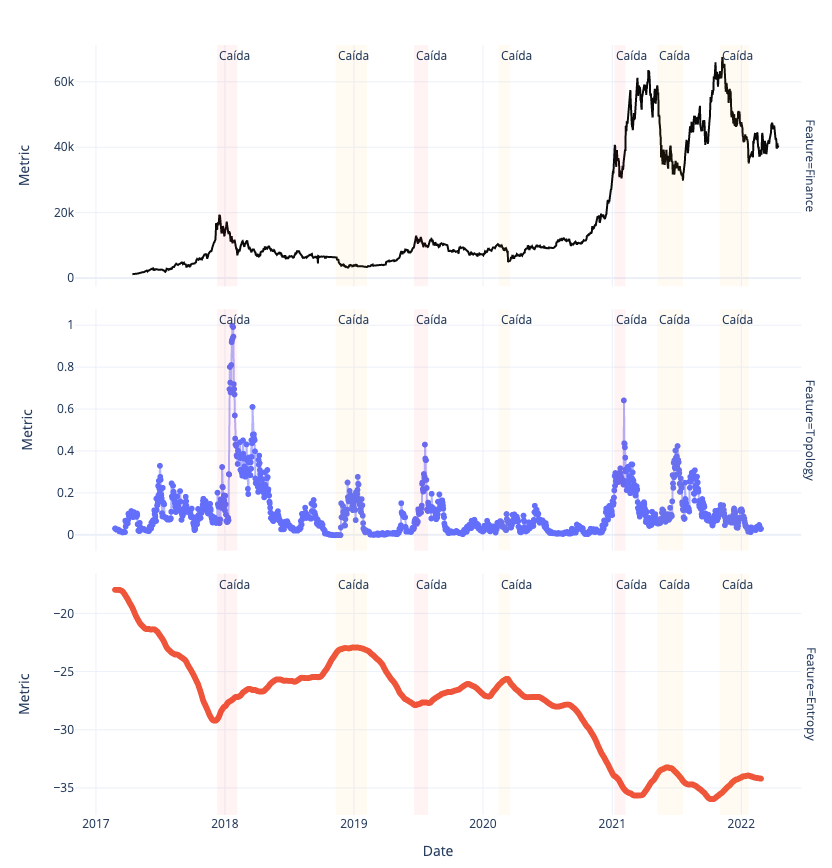
\includegraphics[scale=0.55]{Chapter5/clasifica_transf.png}
	\caption{Características obtenidas de la entropía y el análisis topológico y su relación con las caídas del precio}
	\label{fig27}
\end{figure}
\vspace{1cm}
Como se puede observar en las caídas en rojo, el análisis topológico de datos nos ayuda a prever caídas significativas después de un crecimiento constante en periodos cortos de tiempo. Entre mayor sea la norma $C^1$ mayor será la caída después del aumento del precio. Como se muestra en el crac del 2018, en una semana el precio bajo un 26\% con respecto al actual. A mediados del 2019 el precio sufrió una caída aproximada del 25\% en 7 días mostrando una característica topológica igualmente alta. Por otro lado, a inicios de 2021, del 14 de enero al 21 de enero hubo una caída significativa del 29\% en 7 días. Si se nota la entropía calculada, ésta caracteriza las bajadas del precio con un pequeño valle en la serie de tiempo.

Si la caída ocurre mientras el precio se mantiene relativamente constante o en un periodo largo de tiempo como en los periodos de 2019, 2020, 2021 y 2022 (caídas en naranja) la norma $C^1$ muestra un aumento pero no de forma significativa. La entropía captura mesetas en estos periodos de tiempo que entre más pronunciadas, mayor es la norma $C^1$.
\subsection{Selección de cluster de inversión}

Con las características anteriores se crea un plano que tiene por eje $x$ la entropía normalizada y en el eje $y$ la norma $C^1$ igualmente normalizada. Se agrupan los puntos con el algoritmo K-means de tal forma que estos nos ayuden a detectar las subidas y bajadas del precio para caracterizar la toma de decisiones de inversión como se observa en la \autoref{fig28}.

\begin{figure}[h!]
	\centering
	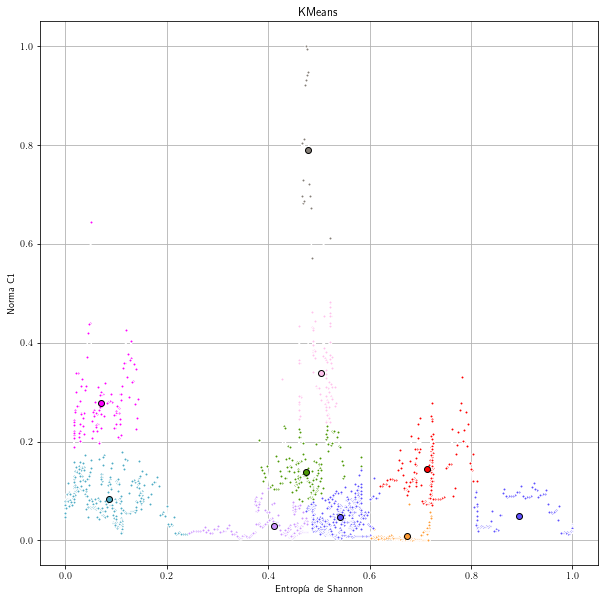
\includegraphics[scale=0.5]{Chapter5/calsifica_kmeans.png}
	\caption{Clusters generados a partir de la entropía y la norma $C^1$ para la toma de decisiones de inversión}
	\label{fig28}
\end{figure}

Estos agrupamientos son llevados a los datos originales donde se lleva a cabo la selección manual de los clusters de comprar, vender o arriesgar. Cuando el precio baja (o hay una caída) se recomienda comprar, cuando sube se recomienda vender

\begin{figure}[h!]
	\centering
	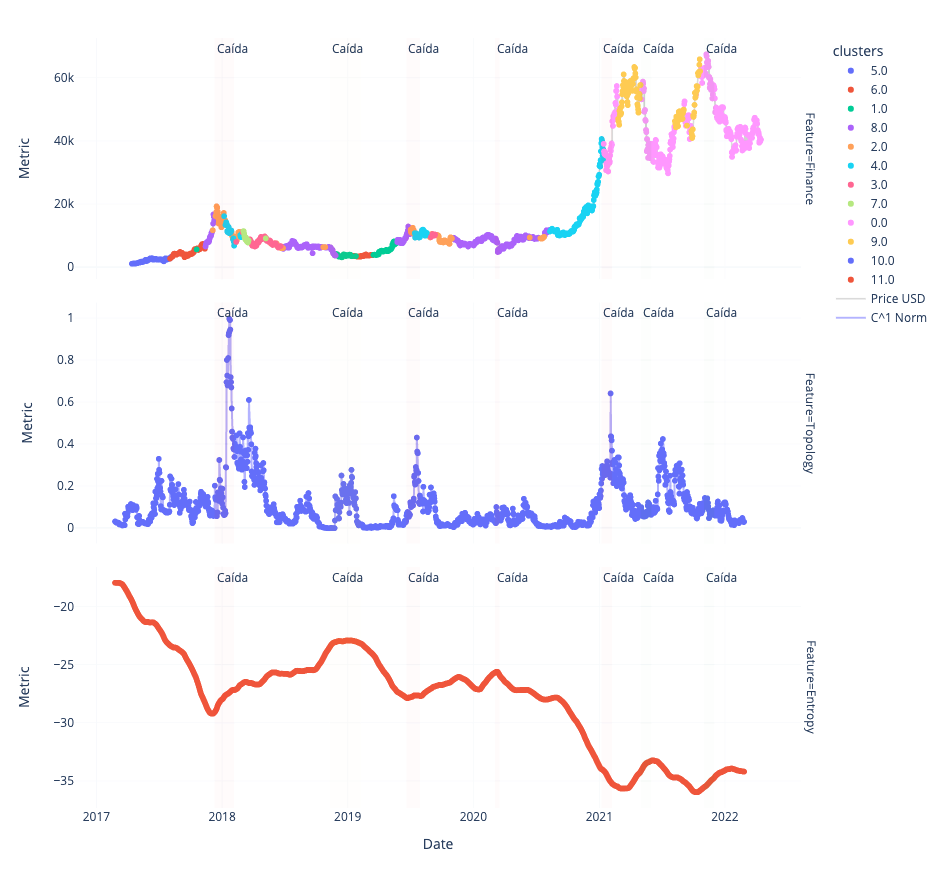
\includegraphics[scale=0.5]{Chapter5/clasifica_inv2.png}
	\caption{Clusters sobre datos del precio originales para la elección manual de los agrupamientos de inversión}
	\label{fig29}
\end{figure}

Los agrupamientos seleccionados para comprar fueron: 2,3,7,0, para vender: 4,5,6,8,9, y arriesgar: 1.
Las imagenes generadas a partir de los datos originales y sus respectivos agrupamientos se muestran en la \autoref{fig30}. 

\begin{figure}[h!]
	\centering
	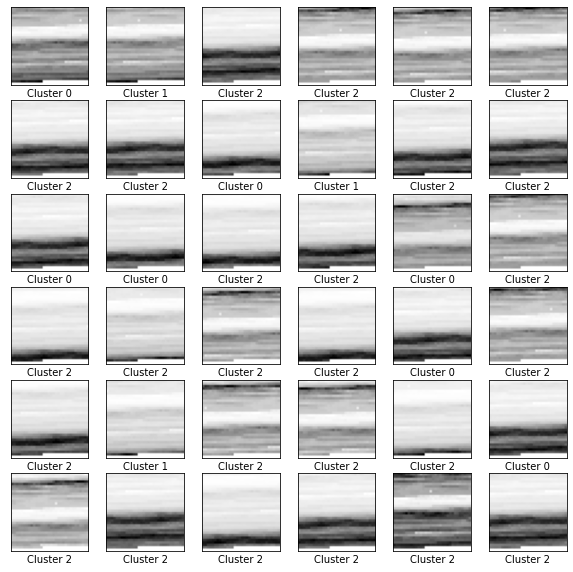
\includegraphics[scale=0.5]{Chapter5/IMG_cluster.png}
	\caption{Imágenes generadas a partir de la serie de tiempo}
	\label{fig30}
\end{figure}

\subsection{Modelo de clasificación}

Despues del entrenamiento con el 80\% de los datos se alcanza una exactitud del 95.76\% sobre los datos de entrenamiento como se observa en la \autoref{fig31}.

\begin{figure}[h!]
	\centering
	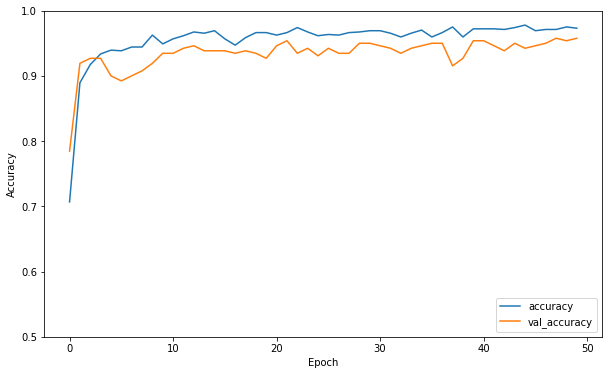
\includegraphics[scale=0.6]{Chapter5/exactitud_clas.png}
	\caption{Exactitud sobre el conjunto de entrenamiento (azul) y el conjunto de prueba (naranja)}
	\label{fig31}
\end{figure}

El modelo es guardado y cargado para realizar predicciones sobre intervalos mayores a 32 días, de tal forma que se realiza una recomendación de inversión utilizando el color rojo para vender, el verde para comprar y el naranja para arriesgar. La linea punteada en la \autoref{fig32} muestran los promedios móviles de 30 días sobre los datos para ayudar a entender mejor la recomendación de inversión. 

\begin{figure}[h!]
	\centering
	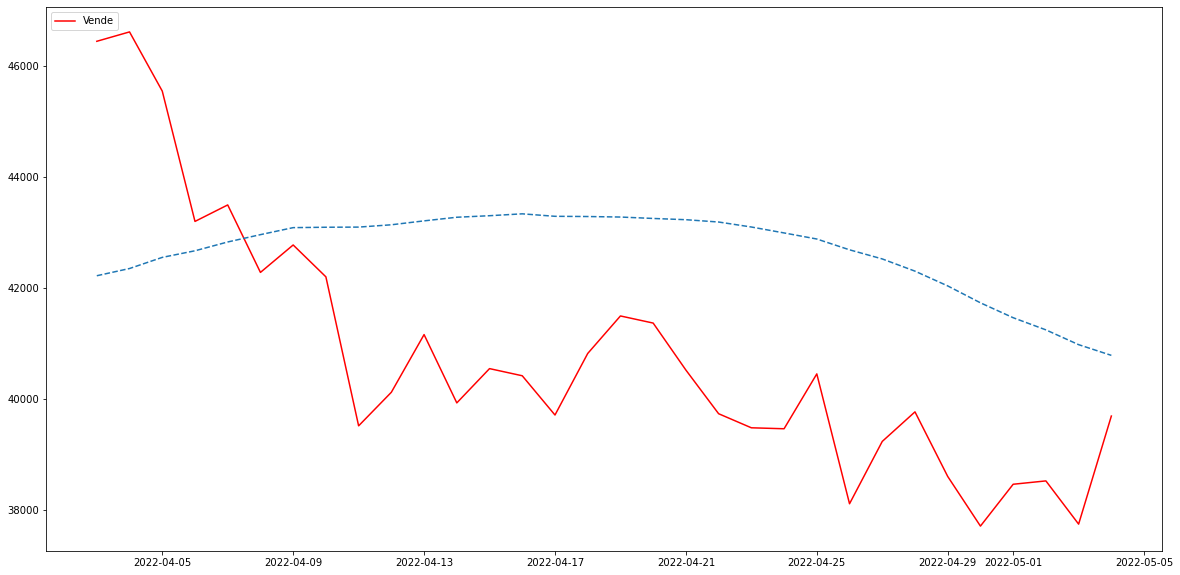
\includegraphics[scale=0.4]{Chapter5/reco.png}
	\caption{Recomendación de inversión del mes de abril a mayo de 2022}
	\label{fig32}
\end{figure}

\begin{figure}[h!]
	\centering
	\subfloat[Crac del 2018]
	{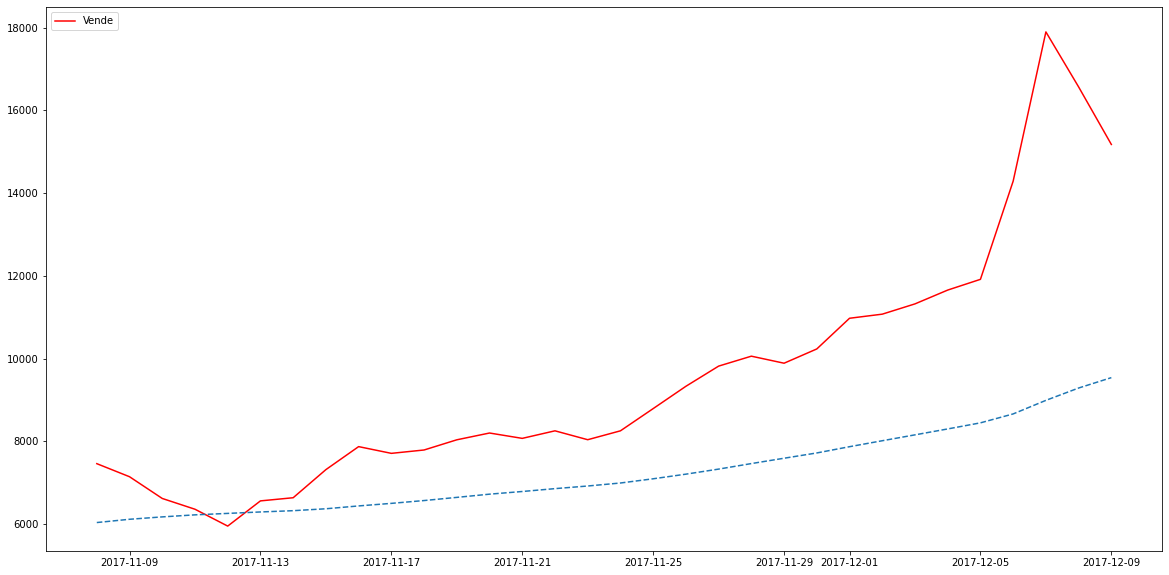
\includegraphics[width=0.47\columnwidth]{Chapter5/2018_crac_vende.png}}
	\qquad
	\subfloat[Mínimos despues del crac del 2018]
	{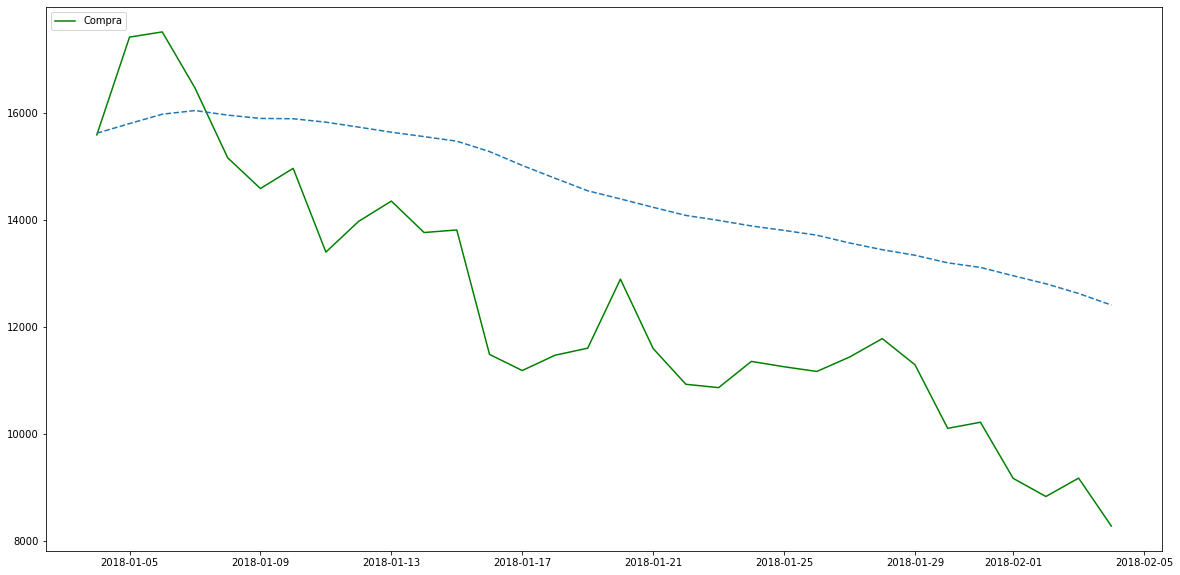
\includegraphics[width=0.47\columnwidth]{Chapter5/2018_crac_compra.png}}
	\qquad
	\subfloat[Crac del mediados del 2021]
	{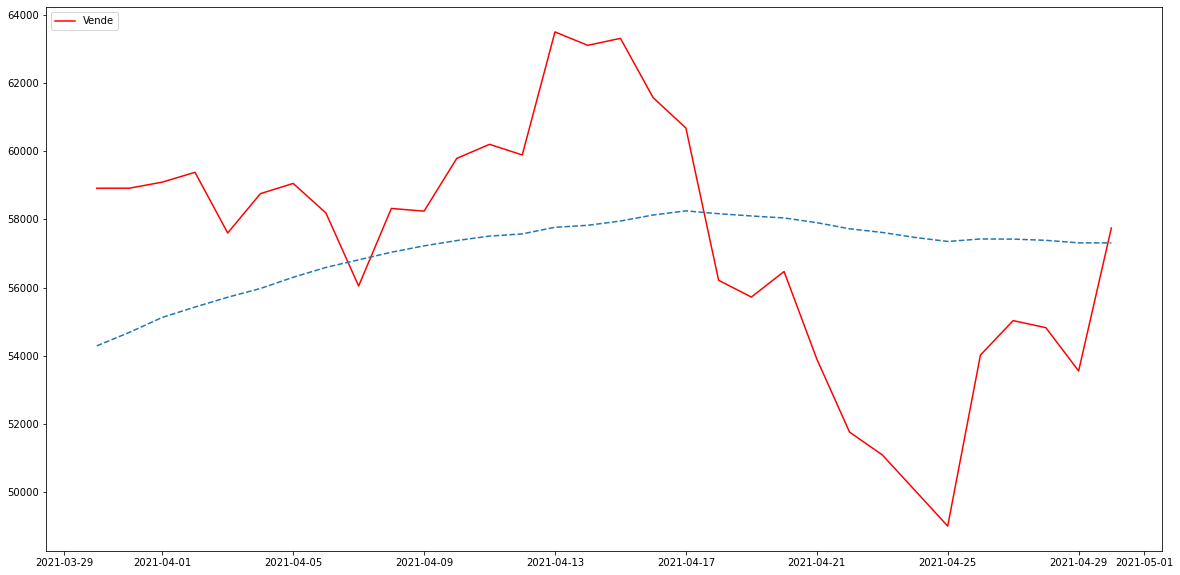
\includegraphics[width=0.47\columnwidth]{Chapter5/2021_crac_vende.png}}
	\qquad
	\subfloat[Mínimos despues del crac del 2021]
	{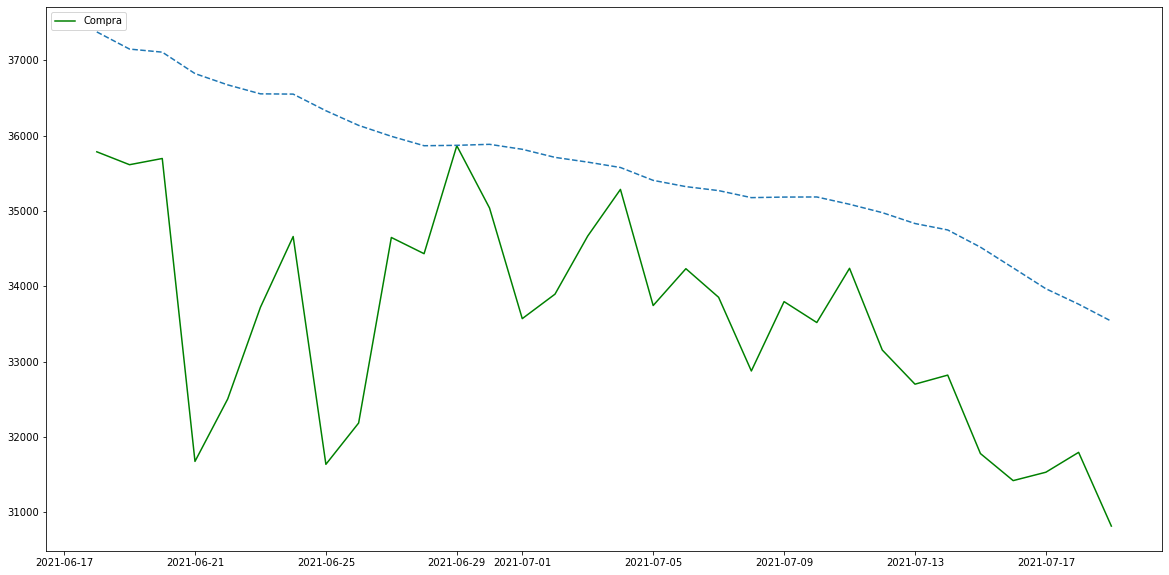
\includegraphics[width=0.47\columnwidth]{Chapter5/2021_crac_compra.png}}
	
	\caption{Recomendaciones de inversión en los intervalos de caídas criticas del precio.}
	\label{fig33}
\end{figure}

En este caso, en un intervalo del cinco de abril al cinco de mayo de 2022, el algoritmo recomienda vender, ocurriendo en los tres días siguientes una caída desde \$39,700 dólares a \$34,500 dólares.

En las caídas drásticas de periodos anteriores  también se realiza una correcta predicción como se muestra en la \autoref{fig33}. Se llega a predecir correctamente y con anticipación el crac de 2018 y 2021 con sus respectivos precios mínimos después de las caídas ayudando a tomar la decisión de realizar una compra.

\chapter[Conclusión]{Conclusiones y trabajo futuro}{Conclusiones y trabajo futuro}\label{Intro}

\noindent
\rule{0.49\textwidth}{0.75pt} $_{\bigcirc}$ \rule{0.49\textwidth}{0.75pt}\\
\lipsum[1]
\lipsum[2]\\
\noindent
\rule{0.49\textwidth}{0.75pt} $_{\bigcirc}$ \rule{0.49\textwidth}{0.75pt}\\
\clearpage

\section{Conclusión}

\lipsum




\end{spacing}


%%% Note that if you want to add more chapters, which might be needed for showing another/more contributory chapters, make a copy of any folder of Chapter2/3 and rename it and include before including the conclusion.

%\renewcommand{\chaptername}{Chapter} %%%%%%%%%%%%%%%%%%%%%%%%%%%%
%
%   \addcontentsline{toc}{chapter}{Index} % added by Sandipan for registering 'Index' in the table of contents
%    \clearpage{\pagestyle{empty}\cleardoublepage}
%    \printindex       % added by Sandipan for printing the index
%    \renewcommand{\chaptername}{Chapter}

%\cmt{
\renewcommand{\chaptername}{Appendix} %%%%%%%%%%%%%%%%%%%%%%%%%%%%
\begin{spacing}{1}
\begin{appendix}
%%%%%%%%%%%%%%%%%%%%%%%%%%%% APPENDIX %%%%%%%%%%%%%%%%%%%%%%%%%%%%
\chapter[Appendix A]{Métricas de la Blockchain}{Métricas de la Blockchain}\label{appen1}
\vskip 10pt
\noindent

\begin{table}[h!]
	\begin{tabular}{|l|m{12cm}|}
		\hline
		\textbf{Métrica}&\textbf{Definición}\\
		\hline
		AdrActCnt         & El recuento de sumas de direcciones únicas que estaban activas en la red (ya sea como destino o fuente de un cambio de libro mayor) ese día. \\
		\hline
		AdrBal1in100KCnt  & La suma de direcciones únicas que poseen al menos una en Xth del suministro actual de unidades nativas al final de ese día                   \\
		\hline
		AdrBal1in100MCnt  & La suma de direcciones únicas que poseen al menos una en Xth del suministro actual de unidades nativas al final de ese día.                  \\
		\hline
		AdrBal1in10BCnt   & La suma de direcciones únicas que poseen al menos una en Xth del suministro actual de unidades nativas al final de ese día.                  \\
		\hline
		AdrBal1in10KCnt   & La suma de direcciones únicas que poseen al menos una en Xth del suministro actual de unidades nativas al final de ese día.                  \\
		\hline
		AdrBal1in10MCnt   & La suma de direcciones únicas que poseen al menos una en Xth del suministro actual de unidades nativas al final de ese día.                  \\
		\hline
		AdrBal1in1BCnt    & La suma de direcciones únicas que poseen al menos una en Xth del suministro actual de unidades nativas al final de ese día.                  \\
		\hline
		AdrBal1in1KCnt    & La suma de direcciones únicas que poseen al menos una en Xth del suministro actual de unidades nativas al final de ese día.                  \\
		\hline
		AdrBal1in1MCnt    & La suma de direcciones únicas que poseen al menos una en Xth del suministro actual de unidades nativas al final de ese día.                  \\
		\hline
		AdrBalCnt         & El recuento de sumas de direcciones únicas que tengan cualquier cantidad de unidades nativas al final de ese día                             \\
		\hline
		AdrBalNtv0.001Cnt & El recuento de sumas de direcciones únicas que tengan al menos X unidades nativas al final de ese día.                                       \\
		\hline
		AdrBalNtv0.01Cnt  & El recuento de sumas de direcciones únicas que tengan al menos X unidades nativas al final de ese día.                                       \\
		\hline
		AdrBalNtv0.1Cnt   & El recuento de sumas de direcciones únicas que tengan al menos X unidades nativas al final de ese día.                                       \\
		\hline
		AdrBalNtv100Cnt   & El recuento de sumas de direcciones únicas que tengan al menos X unidades nativas al final de ese día.\\
		\hline                                     
	\end{tabular}
\end{table}

\newpage
\begin{table}[h!]
	\begin{tabular}{|l|m{12cm}|}
		\hline
		\textbf{Métrica}&\textbf{Definición}\\
		\hline
		AdrActCnt         & El recuento de sumas de direcciones únicas que estaban activas en la red (ya sea como destino o fuente de un cambio de libro mayor) ese día. \\
		\hline
		AdrBal1in100KCnt  & La suma de direcciones únicas que poseen al menos una en Xth del suministro actual de unidades nativas al final de ese día                   \\
		\hline
		AdrBal1in100MCnt  & La suma de direcciones únicas que poseen al menos una en Xth del suministro actual de unidades nativas al final de ese día.                  \\
		\hline
		AdrBal1in10BCnt   & La suma de direcciones únicas que poseen al menos una en Xth del suministro actual de unidades nativas al final de ese día.                  \\
		\hline
		AdrBal1in10KCnt   & La suma de direcciones únicas que poseen al menos una en Xth del suministro actual de unidades nativas al final de ese día.                  \\
		\hline
		AdrBal1in10MCnt   & La suma de direcciones únicas que poseen al menos una en Xth del suministro actual de unidades nativas al final de ese día.                  \\
		\hline
		AdrBal1in1BCnt    & La suma de direcciones únicas que poseen al menos una en Xth del suministro actual de unidades nativas al final de ese día.                  \\
		\hline
		AdrBal1in1KCnt    & La suma de direcciones únicas que poseen al menos una en Xth del suministro actual de unidades nativas al final de ese día.                  \\
		\hline
		AdrBal1in1MCnt    & La suma de direcciones únicas que poseen al menos una en Xth del suministro actual de unidades nativas al final de ese día.                  \\
		\hline
		AdrBalCnt         & El recuento de sumas de direcciones únicas que tengan cualquier cantidad de unidades nativas al final de ese día                             \\
		\hline
		AdrBalNtv0.001Cnt & El recuento de sumas de direcciones únicas que tengan al menos X unidades nativas al final de ese día.                                       \\
		\hline
		AdrBalNtv0.01Cnt  & El recuento de sumas de direcciones únicas que tengan al menos X unidades nativas al final de ese día.                                       \\
		\hline
		AdrBalNtv0.1Cnt   & El recuento de sumas de direcciones únicas que tengan al menos X unidades nativas al final de ese día.                                       \\
		\hline
		AdrBalNtv100Cnt   & El recuento de sumas de direcciones únicas que tengan al menos X unidades nativas al final de ese día.\\
		\hline
	\end{tabular}
	\caption{Métricas de la blockchain y su definición.}
	\label{tab:TableAppen1}                                     
\end{table}

%	\begin{table}
%			\centering
%			\begin{tabular}{p{5cm} p{5cm}  }
%				\toprule
%				\textbf{ID} & \textbf{ID}\\
%				\midrule
%				AdrActCnt  &  AdrBal1in100KCnt \\
%				AdrBal1in100MCnt & AdrBal1in10BCnt \\
%				AdrBal1in10KCnt & AdrBal1in10MCnt \\
%				AdrBal1in1BCnt & AdrBal1in1KCnt \\
%				AdrBal1in1MCnt & AdrBalCnt \\
%				AdrBalNtv0.001Cnt & AdrBalNtv0.01Cnt\\
%				AdrBalNtv0.1Cnt & AdrBalNtv100Cnt \\
%				AdrBalNtv100KCnt & AdrBalNtv10Cnt\\
%				AdrBalNtv10KCnt & AdrBalNtv1Cnt \\
%				AdrBalNtv1KCnt & AdrBalNtv1MCnt \\
%				AdrBalUSD100Cnt & AdrBalUSD100KCnt \\
%				AdrBalUSD10Cnt & AdrBalUSD10KCnt \\
%				AdrBalUSD10MCnt & AdrBalUSD1Cnt \\ 
%				AdrBalUSD1KCnt & AdrBalUSD1MCnt \\
%				AssetEODCompletionTime & BlkCnt \\
%				BlkSizeMeanByte & BlkWghtMean \\
%				BlkWghtTot & CapAct1yrUSD \\
%				CapMVRVCur & CapMVRVFF \\
%				CapMrktCurUSD & CapMrktFFUSD \\
%				CapRealUSD & DiffLast \\
%				DiffMean & FeeByteMeanNtv \\
%				FeeMeanNtv & FeeMeanUSD \\
%				FeeMedNtv & FeeMedUSD \\
%				FeeTotNtv & FeeTotUSD \\
%				FlowInExNtv & FlowInExUSD \\
%				FlowOutExNtv & FlowOutExUSD \\
%				FlowTfrFromExCnt & HashRate \\
%				HashRate30d & IssContNtv \\
%				IssContPctAnn & IssContPctDay \\
%				IssContUSD & IssTotNtv \\
%				IssTotUSD & NDF,NVTAdj \\
%				NVTAdj90 & NVTAdjFF \\
%				NVTAdjFF90 & PriceBTC \\
%				PriceUSD & ROI1yr \\
%				ROI30d & RevAllTimeUSD \\
%				RevHashNtv & RevHashRateNtv \\
%				RevHashRateUSD & RevHashUSD \\
%				RevNtv & RevUSD \\
%				SER & SplyAct10yr \\
%				SplyAct180d & SplyAct1d \\
%				SplyAct1yr & SplyAct2yr \\
%				SplyAct30d & SplyAct3yr \\
%				SplyAct4yr & SplyAct5yr \\
%				SplyAct7d & SplyAct90d \\
%				SplyActEver & SplyActPct1yr \\
%				SplyAdrBal1in100K & SplyAdrBal1in100M \\
%				SplyAdrBal1in10B & SplyAdrBal1in10K \\
%				SplyAdrBal1in10M & SplyAdrBal1in1B \\
%				SplyAdrBal1in1K & SplyAdrBal1in1M \\
%				SplyAdrBalNtv0.001 & SplyAdrBalNtv0.01 \\
%				SplyAdrBalNtv0.1 & SplyAdrBalNtv1 \\
%				SplyAdrBalNtv10 & SplyAdrBalNtv100 \\
%				SplyAdrBalNtv100K & SplyAdrBalNtv10K \\
%				SplyAdrBalNtv1K & SplyAdrBalNtv1M \\
%				SplyAdrBalUSD1 & SplyAdrBalUSD10 \\
%				SplyAdrBalUSD100 & SplyAdrBalUSD100K \\
%				SplyAdrBalUSD10K & SplyAdrBalUSD10M \\
%				SplyAdrBalUSD1K & SplyAdrBalUSD1M \\
%				SplyAdrTop100 & SplyAdrTop10Pct \\
%				SplyAdrTop1Pct & SplyCur \\
%				SplyExpFut10yr & SplyFF \\
%				SplyMiner0HopAllNtv & SplyMiner0HopAllUSD \\
%				SplyMiner1HopAllNtv & SplyMiner1HopAllUSD \\
%				TxCnt & TxCntSec \\
%				TxTfrCnt & TxTfrValAdjNtv \\
%				TxTfrValAdjUSD & TxTfrValMeanNtv \\
%				TxTfrValMeanUSD & TxTfrValMedNtv \\
%				TxTfrValMedUSD & VelCur1yr \\
%				VtyDayRet180d & VtyDayRet30d\\
%				\bottomrule \\
%				\end{tabular}
%			\caption{Métricas utilizadas en el estudio.}
%			\label{tab:Table11}
%			\end{table}





%\chapter[Appendix A]{Legendre Polynomials}{Legendre Polynomials}\label{appen1}
\begin{spacing}{1.25}
\vskip 20pt
\noindent
\rule{0.49\textwidth}{0.75pt} $_{\Diamond}$ \rule{0.49\textwidth}{0.75pt}\\
{\Large{\textbf{Preface}}}\\
\\
\rule{0.49\textwidth}{0.75pt} $_{\Diamond}$ \rule{0.49\textwidth}{0.75pt}
\end{spacing}
\newpage

\textbf{Legendre's Differential Equation and Its Solution}\\\\


\rule{0.46\textwidth}{0.75pt} $_{\Diamond}$ \rule{0.46\textwidth}{0.75pt}\\



\chapter[Metodología del estado del arte]{Metodología del estado del arte}{Metodología del estado del arte}\label{appen3}
\renewcommand{\tablename}{Tabla}


\section{Metodología SLR}

La revisión sistemática de literatura (SLR) es un método que nos permite interpretar y sintetizar de forma adecuada la información obtenida de un tema de investigación. Dado que se ejecuta una manera sistemática sus ventajas son un incremento en la posibilidad de tener mejores resultados en la búsqueda de información \parencite{kitchenhamSystematicLiteratureReviews2009}. Hay tres fases principales en una SLR: (1) Planificación de revisión, (2) Realización de la revisión, (3) Reporte de resultados.

\paragraph{Planificación de revisión}

Esta fase se centra en: (1) La identificación de la necesidad de realizar el SLR, (2) formular las preguntas de investigación que guían la ejecución del SLR, (3) generar la búsqueda de cadenas, y (4) la selección de las fuentes de información para la extracción de los estudios primarios.

\paragraph{Realización de la revisión}

La segunda fase del SLR corresponde a la definición de los criterios de inclusión y exclusión, la ejecución de un proceso de selección de estudios y la evaluación de la calidad de los mismos, lo que da lugar a la selección de los estudios primarios.\\

La metodología se aplicará a tres factores clave de la tesis: el pronóstico del precio, análisis de métricas de la blockchain y la clasificación de precios de la criptomoneda. 


\section{Pronóstico del precio del bitcoin}

\subsection{Planificación de revisión}
\subsubsection{Identificar la necesidad de realizar el SLR}
Tener un enfoque sistemático a la hora de comparar y escoger un algoritmo para la predicción del bitcoin es crucial por la cantidad de datos e información que se pueden obtener hoy día con actualización constante. Una buena comprensión de las variables explicativas, formateo de datos y métodos para comparar los modelos es fundamental a la hora de comprender el modelo propuesto.

\subsubsection{Definiendo las preguntas de investigación}
Las preguntas de investigación para este estudio son las siguientes:

\begin{itemize}
	\item ¿Cuál es el estado del arte de modelos estadísticos para pronósticos del bitcoin?
	\item ¿Cómo implementar trading con bitcoin?
	\item ¿Cuales son los modelos de pronósticos más utilizados?
	\item ¿Qué modelos de aprendizaje máquina se están utilizando?
	\item ¿Cuál es el mejor modelo para realizar pronóstico del bitcoin?
\end{itemize}

\subsubsection{Generar las cadenas de búsqueda}
Para facilitar la búsqueda de los estudios primarios se identificaron las palabras clave resultantes de las preguntas de investigación. Resultaron en las siguientes:

\begin{itemize}
	\item Bitcoin
	\item Machine learning
	\item Trading
	\item Forecasting
\end{itemize}

Combinando las palabras clave con el uso de conectores lógicos “AND” y “OR”, la siguiente cadena de búsqueda es obtenida:\\

\centerline{Bitcoin \textbf{AND} (machine learning \textbf{OR} trading \textbf{OR} forecasting)}

\subsubsection{Selección de fuentes de información}
Las siguientes fuentes de información fueron seleccionadas para la extracción de los estudios:
\begin{itemize}
	\item Google Scholar
	\item IEEE Xplorer
	\item ELSEVIER Science
	\item Springer Link
\end{itemize}

\subsection{Realización de la revisión}
\subsubsection{Criterio de inclusión y exclusión}
Para filtrar los estudios no relevantes para esta investigación se definen los criterios de inclusión y exclusión, que da lugar a los presentados en la \autoref{tab:Table1}.

\begin{table}[h!]
	\centering
	\begin{tabular}{ | m{7cm}| m{7cm} | }
		\hline
		\textbf{Criterio de inclusión} & \textbf{Criterio de exclusión}\\
		\hline
		
		Los primeros estudios mas relevantes según los filtros de búsqueda de las fuentes de información seleccionadas.& Estudios no relevantes según los filtros de búsqueda de las fuentes de información.\\
		
		\hline
		El título contiene la palabra clave ``Bitcoin'' y al menos otra palabra clave. &  El título no contiene ninguna palabra clave\\ 
		\hline
		Abstract está relacionado con predicción de precios del bitcoin usando machine learning o métodos estadísticos. & Estudios que no están relacionados con la predicción del
		bitcoin.\\
		\hline
		Estudios que contienen enfoques de metodologías, modelos, métodos, técnicas de predicción del bitcoin. & Estudios relacionados con el bitcoin pero no tienen un
		enfoque en ciencia de datos.\\
		\hline
		Estudios que contengan resultados sobre la predicción del precio del bitcoin con sus respectivos indicadores de error y comparación con otros métodos. & Estudios con resultados sobre la predicción del bitcoin pero sin comparación de modelos.\\
		\hline
		Estudios publicados entre 2016 y 2020. & Estudios publicados antes del 2016.\\
		\hline
	\end{tabular}
	\caption{Criterios de inclusión y exclusión}
	\label{tab:Table1}
\end{table}

\subsubsection{Selección de estudios primarios}
El protocolo SLR \parencite{kitchenhamSystematicLiteratureReviews2009} sugiere definir un proceso de selección de estudios para obtener los estudios primarios, estructurado de la siguiente manera: (1) aplicar y adaptar la cadena de búsqueda a cada fuente de datos, (2) filtrar los estudios aplicando los primeros criterios de inclusión a cada fuente de información, (3) aplicar el resto de los criterios de inclusión y exclusión, y (4) seleccionar los estudios primarios. Después de aplicar los criterios de inclusión y exclusión como parte del proceso de selección de estudios, se seleccionaron 8 estudios primarios para esta investigación como se ve en la \autoref{fig1}.\\

\begin{figure}[!h]
	\centering
	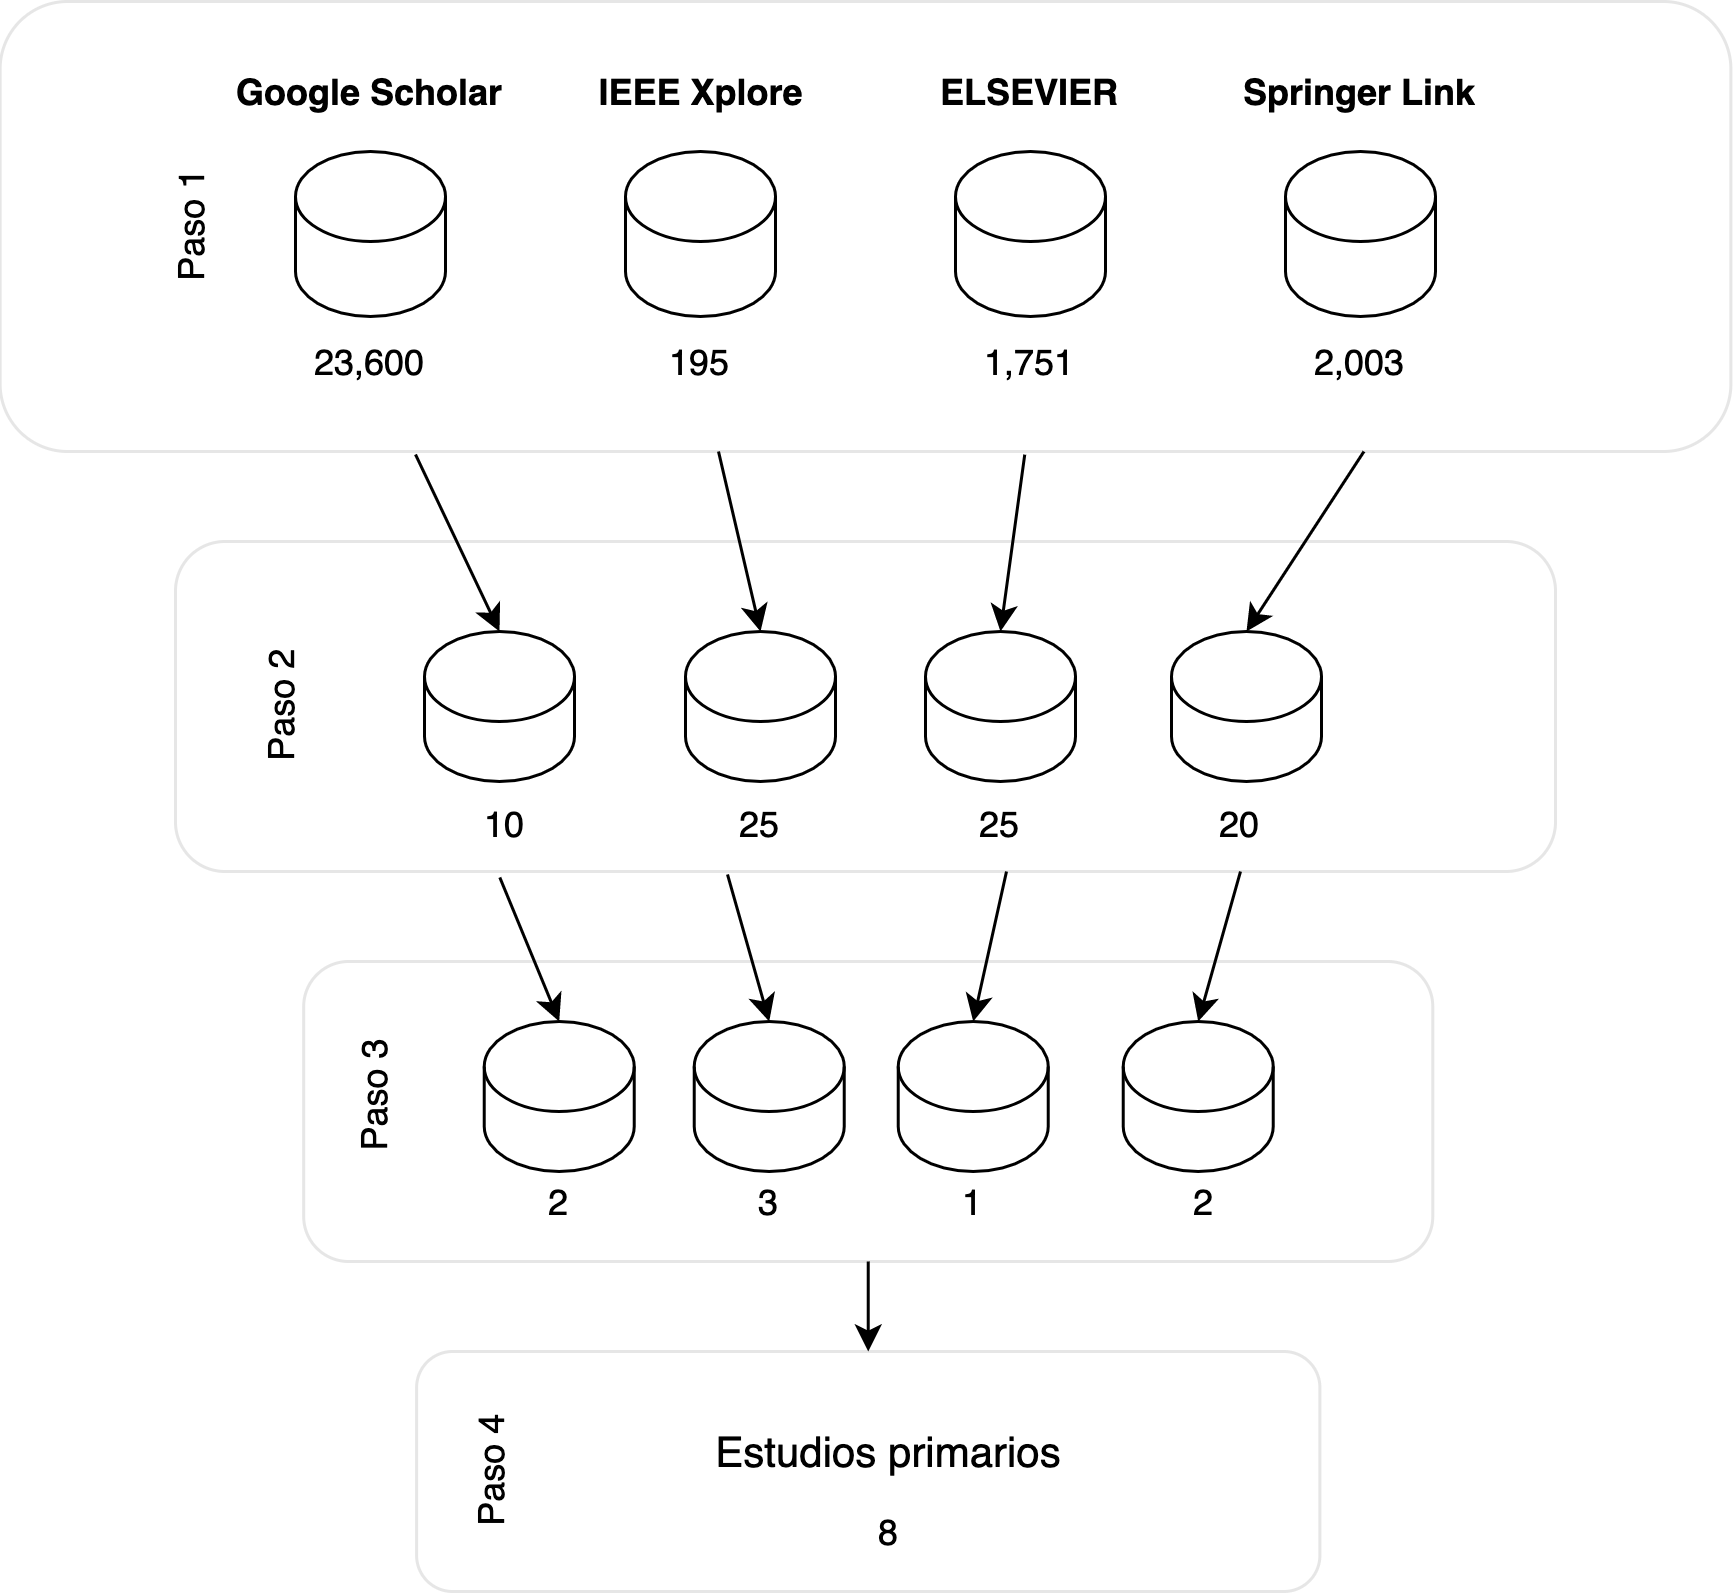
\includegraphics[width=0.7\linewidth]{Chapter2/SelecEstudiPrim_1.png}
	\caption{Selección de estudios primarios y resultados}
	\label{fig1}
\end{figure}

\vspace{-0.5cm}

\subsubsection{Evaluación de la calidad del estudio}
Al evaluar la calidad del estudio, se garantiza que la información contenida en cada uno de los estudios primarios sea pertinente y valiosa para la investigación. En la \autoref{tab:Table2} se presenta la evaluación de la calidad de los estudios que se aplicarán.

\begin{table}[!h]
	\centering
	\begin{tabular}{ | m{2cm}| m{12cm} | }
		\hline
		\textbf{ID} & \textbf{Evaluación de la calidad del estudio}\\
		\hline
		PC1 & ¿El estudio cuenta con una base teórica que explique los métodos utilizados?\\
		\hline
		PC2 & ¿El estudio detalla el método con el cuál pronostica y que variables explicativas utiliza para hacer la predicción?\\
		\hline
		PC3 & ¿El estudio compara modelos de predicción para pronosticar el precio del bitcoin?\\
		\hline
		PC4 & ¿El estudio utiliza algoritmos de machine learning para realizar la predicción?\\
		\hline
		PC5 & ¿El estudio muestra un modelo con mejor rendimiento comparado con los demás?\\
		\hline
	\end{tabular}
	\caption{Evaluación de la calidad del estudio}
	\label{tab:Table2}
\end{table}

Después de evaluar los estudios primarios utilizando las evaluaciones de calidad antes mencionadas quedaron \textbf{6 estudios primarios} \parencite{tandonBitcoinPriceForecasting2019,chenBitcoinPricePrediction2020,mudassirTimeseriesForecastingBitcoin2020,felizardoComparativeStudyBitcoin2019,mcnallyPredictingPriceBitcoin2018,phaladisailoedMachineLearningModels2018}.

\section{Análisis de métricas de la blockchain}
\subsection{Planificación de revisión}
\subsubsection{Identificar la necesidad de realizar el SLR}

Tener un enfoque sistemático de las métricas que más influyen en el precio del bitcoin es crucial por la cantidad de datos e información que se pueden obtener hoy día con actualización constante, más tratándose de un campo tecnológico con evolución persistente.
Una buena comprensión de las variables explicativas ayuda a mejorar y ahorrar esfuerzos en el entendimiento del asenso y descenso del precio de esta criptomoneda.

\subsubsection{Definiendo las preguntas de investigación}
Las preguntas de investigación son las siguientes:
\begin{itemize}
	\item ¿Con qué métodos se están seleccionando las mejores métricas de la blockchain para predicción del precio?
	\item Actualmente, ¿cuales son las métricas de la blockchain que más influyen en el precio del bitcoin?
	\item ¿Cuánto mejora la predicción con las métricas de la blockchain?
\end{itemize}

\subsubsection{Generar las cadenas de búsqueda}
Para facilitar la búsqueda de los estudios primarios se identificaron las palabras clave resultantes de las preguntas de investigación. Resultaron en las siguientes:
\begin{itemize}
	\item Bitcoin
	\item Blockchain
	\item Metrics
	\item Prediction
	\item Features
\end{itemize}
Combinando las palabras clave con el uso de conectores lógicos “AND” y “OR”, la siguiente cadena de búsqueda es obtenida:\\

\centerline{(Bitcoin \textbf{AND} blockchain \textbf{AND} metrics \textbf{AND} prediction)} 
\centerline{\textbf{OR} (Bitcoin \textbf{AND} features \textbf{AND} prediction)}

\subsubsection{Selección de fuentes de información}
Las siguientes fuentes de información fueron seleccionadas para la extracción de los estudios:\\
\vspace{-1cm}
\begin{itemize}
	\item IEEE Xplore
	\item ELSEVIER Science Direct
	\item Springer Link\\
\end{itemize}
\vspace{-1.5cm}
\subsection{Realización de la revisión}
\subsubsection{Criterio de inclusión y exclusión}
Para filtrar los estudios no relevantes para esta investigación se definen los criterios de inclusión y exclusión, que da lugar a los presentados en la \autoref{tab:Table3}.\\

\begin{table}[h!]
	\centering
	\begin{tabular}{ | m{7cm}| m{7cm} | }
		\hline
		\textbf{Criterio de inclusión} & \textbf{Criterio de exclusión}\\
		\hline
		Los primeros estudios más relevantes según los filtros de búsqueda de las fuentes de información seleccionadas.& Estudios no relevantes según los filtros de búsqueda de las fuentes de información.\\
		\hline
		El titulo contiene la palabra Bitcoin o Blockchain y al menos otra palabra clave.&  El titulo no contiene ninguna palabra clave.\\ 
		\hline
		El estudio muestra el o los método utilizados para la selección de métricas.& El estudio no muestra el o los métodos utilizados para la selección de métricas.\\
		\hline
		Estudios publicados entre 2017-2021&Estudios publicados antes del 2017.\\
		\hline
	\end{tabular}
	\caption{Criterios de inclusión y exclusión}
	\label{tab:Table3}
\end{table}

\begin{figure}[H]
	\centering
	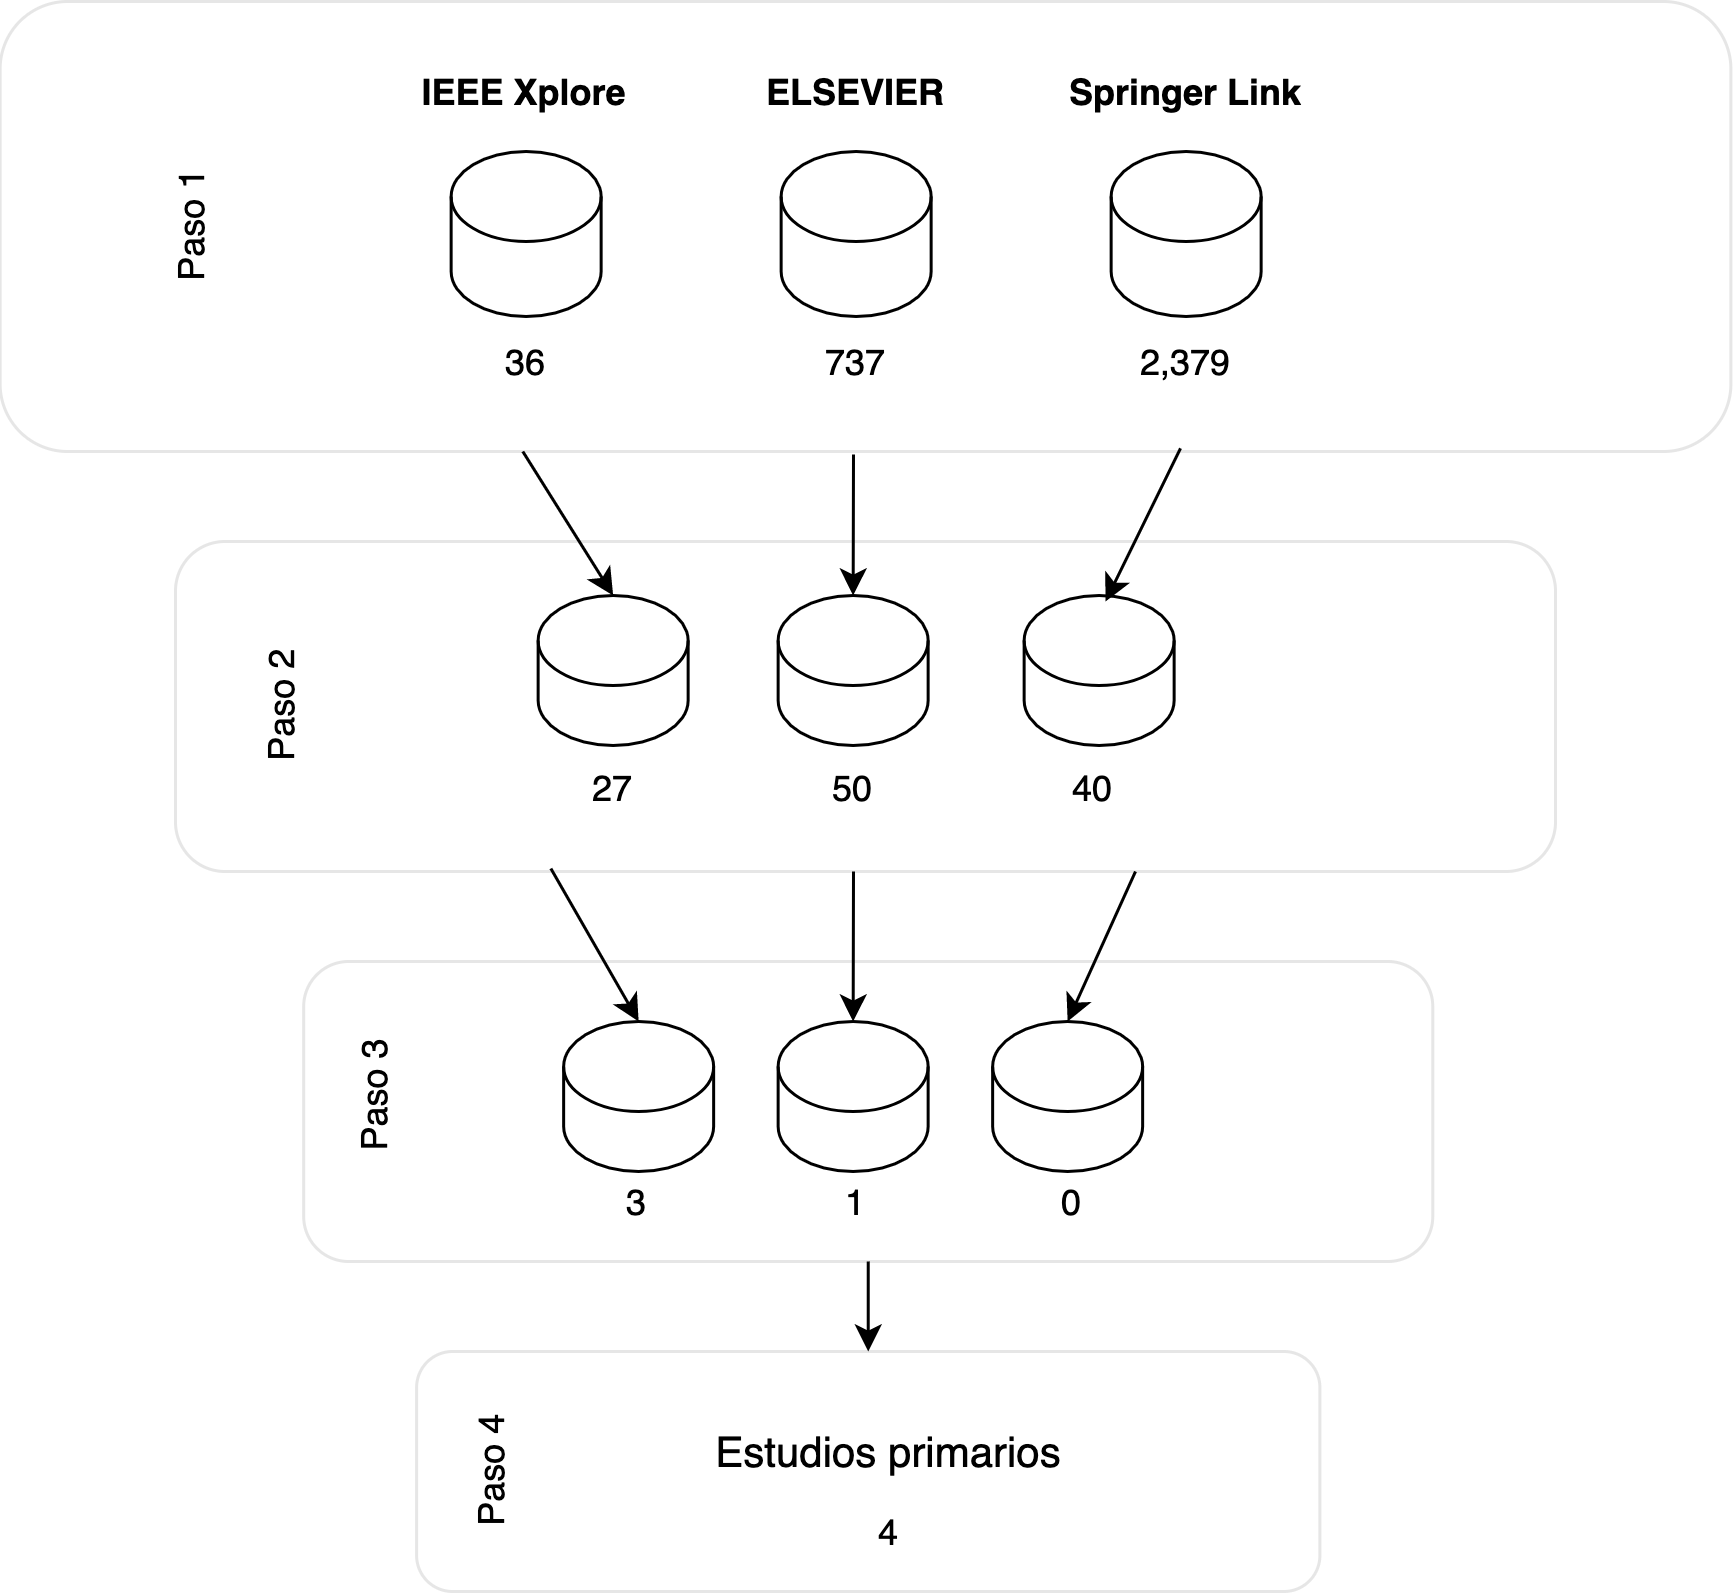
\includegraphics[width=0.7\textwidth]{Chapter2/SelecEstudiPrim_2.png}
	\caption{Selección de estudios primarios y resultados}
	\label{fig2}
\end{figure}
\vspace{-0.8cm}
\subsubsection{Selección de estudios primarios}
Después de aplicar los criterios de inclusión y exclusión como parte del proceso de selección de estudios, se seleccionaron 4 estudios primarios para esta investigación como se ve en la \autoref{fig2}.\\
\vspace{-1cm}
\subsubsection{Evaluación de la calidad del estudio}
Al evaluar la calidad del estudio, se garantiza que la información contenida en cada uno de los estudios primarios sea pertinente y valiosa para la investigación. En la \autoref{tab:Table5} se presenta la evaluación de la calidad de los estudios que se aplicarán.

\begin{table}[H]
	\centering
	\begin{tabular}{ | m{2cm}| m{12cm} | }
		\hline
		\textbf{ID} & \textbf{Evaluación de la calidad del estudio}\\
		\hline
		PC1 & ¿El estudio detalla y explica la metodología utilizada para encontrar las variables explicativas que mejoran la predicción?\\
		\hline
		PC2 & ¿El estudio concluye si agregar variables de la blockchain mejora o no la predicción del bitcoin?\\
		\hline
	\end{tabular}
	\caption{Evaluación de la calidad del estudio}
	\label{tab:Table5}
\end{table}

Después de evaluar los estudios primarios utilizando las evaluaciones de calidad antes mencionadas quedaron 3 estudios primarios \parencite{chenMachineLearningModel2021,jiBestFeatureSelection2019,saadCharacterizingBlockchainbasedCryptocurrencies2018}.

\section{Clasificación del precio para inversión}

\subsection{Planificación de revisión}
\subsubsection{Identificar la necesidad de realizar el SLR}

Un enfoque sistemático de los métodos de clasificación más utilizados es de suma importancia ya que por la existencia de una gran variedad de métodos y cambios constantes en los mismos con un ritmo acelerado pude ser abrumador, por lo anterior el entendimiento de los modelos de clasificación con un enfoque SLR puede impulsar la creación de nuevos modelos más robustos y con mejor precisión.\\

\subsubsection{Definiendo las preguntas de investigación}
Las preguntas de investigación para este estudio son las siguientes:
\begin{itemize}
	\item ¿Qué modelos de clasificación se están utilizando?
	\item ¿Cómo se clasifican los precios del bitcoin para la toma de decisiones de inversión?
	\item ¿Cuál es la mejor metodología para clasificación de precios del bitcoin?
\end{itemize}

\subsubsection{Generar las cadenas de búsqueda}
Para facilitar la búsqueda de los estudios primarios se identificaron las palabras clave resultantes de las preguntas de investigación. Resultaron en las siguientes:
\begin{itemize}
	\item Bitcoin
	\item Blockchain
	\item Investment
	\item Classification
	\item Deep Learning
\end{itemize}
Combinando las palabras clave con el uso de conectores lógicos “AND” y “OR”, la siguiente cadena de búsqueda es obtenida:\\

\centerline{(Bitcoin \textbf{AND} classification \textbf{AND} deep learning)} 
\centerline{\textbf{OR} (Bitcoin \textbf{AND} classification \textbf{AND} deep learning \textbf{AND} investment)}

\subsubsection{Selección de fuentes de información}
Las siguientes fuentes de información fueron seleccionadas para la extracción de los estudios:\\
\begin{itemize}
	\item IEEE Xplore
	\item ELSEVIER Science Direct
	\item Springer Link\\
\end{itemize}
\subsection{Realización de la revisión}
\subsubsection{Criterio de inclusión y exclusión}
Para filtrar los estudios no relevantes para esta investigación se definen los criterios de inclusión y exclusión, que da lugar a los presentados en la \autoref{tab:Table6}.\\

\begin{table}[h!]
	\centering
	\begin{tabular}{ | m{7cm}| m{7cm} | }
		\hline
		\textbf{Criterio de inclusión} & \textbf{Criterio de exclusión}\\
		\hline
		Los primeros estudios más relevantes según los filtros de búsqueda de las fuentes de información seleccionadas.& Estudios no relevantes según los filtros de búsqueda de las fuentes de información.\\
		\hline
		El titulo contiene la palabra Bitcoin o Blockchain y al menos otra palabra clave.&  El titulo no contiene ninguna palabra clave.\\ 
		\hline
		El abstract está relacionado con la clasificación del precios del Bitcoin.& Estudios que no estaban relacionados con la clasificación del precio del bitcoin.\\
		\hline
		Estudios que contienen resultados sobre la clasificación de precios del Bitcoin con sus respectivos indicadores de precisión.& Estudios que no muestran indicadores de precisión de la clasificación.\\
		\hline
		Estudios publicados entre 2017-2021&Estudios publicados antes del 2017.\\
		\hline
	\end{tabular}
	\caption{Criterios de inclusión y exclusión}
	\label{tab:Table6}
\end{table}

\begin{figure}[h!]
	\centering
	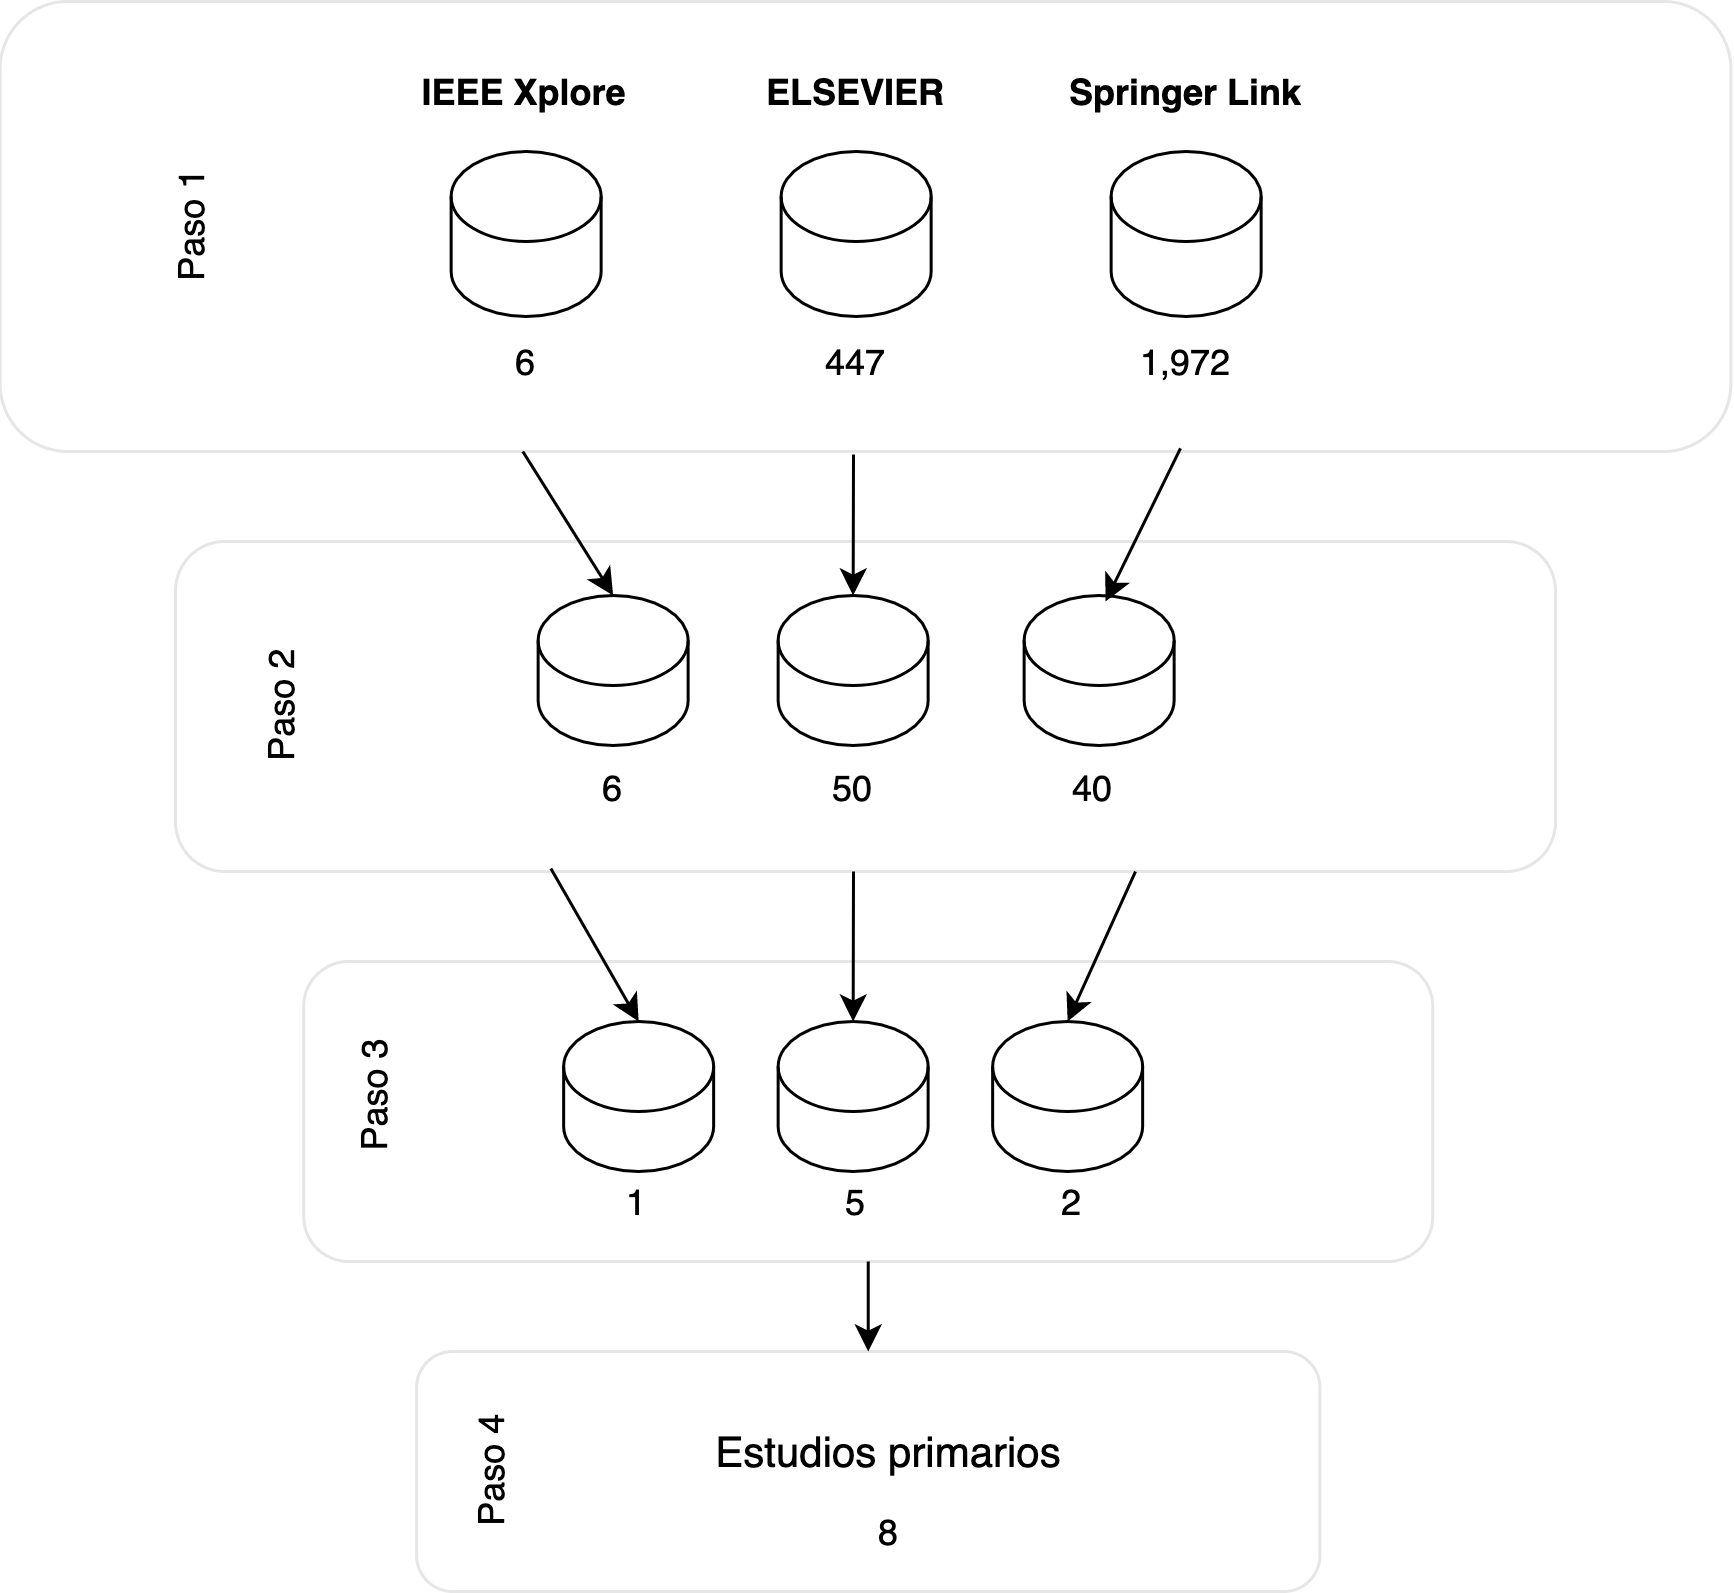
\includegraphics[width=0.7\textwidth]{Chapter2/SelecEstudiPrim_3.png}
	\caption{Selección de estudios primarios y resultados}
	\label{fig3}
\end{figure}

\subsubsection{Selección de estudios primarios}
Después de aplicar los criterios de inclusión y exclusión como parte del proceso de selección de estudios, se seleccionaron 8 estudios primarios para esta investigación como se ve en la \autoref{fig3}.\\

\subsubsection{Evaluación de la calidad del estudio}
Al evaluar la calidad del estudio, se garantiza que la información contenida en cada uno de los estudios primarios sea pertinente y valiosa para la investigación. En la \autoref{tab:Table7} se presenta la evaluación de la calidad de los estudios que se aplicarán.

\begin{table}[H]
	\centering
	\begin{tabular}{ | m{2cm}| m{12cm} | }
		\hline
		\textbf{ID} & \textbf{Evaluación de la calidad del estudio}\\
		\hline
		PC1 & ¿El estudio detalla la metodología utilizada para realizar la clasificación de los precios?\\
		\hline
		PC2 & ¿El estudio da una descripción de los modelos utilizados para realizar la clasificación?\\
		\hline
		PC3 & ¿El estudio muestra un modelo de clasificación con un mejor rendimiento comparado con los demás?\\
		\hline
	\end{tabular}
	\caption{Evaluación de la calidad del estudio}
	\label{tab:Table7}
\end{table}

Después de evaluar los estudios primarios utilizando las evaluaciones de calidad antes mencionadas quedaron 5 estudios primarios \parencite{ibrahimPredictingMarketMovement2021,jaquartShorttermBitcoinMarket2021,chenBitcoinPricePrediction2020,akyildirimPredictionCryptocurrencyReturns2021,pintelasInvestigatingProblemCryptocurrency2020}.

\section{Discusión de la metodología SLR}
En esta sección daremos respuesta a nuestras preguntas de investigación con base en los artículos primarios.

\subsection{Pronóstico del precio del bitcoin}

\textbf{\textit{1.- ¿Cuál es el estado del arte de modelos estadísticos para pronósticos de bitcoin?}}\\
Bitcoin es una criptomoneda altamente usada hoy día, por ello hay algunos modelos para la predicción de su precio, ya sea con modelos estadísticos más tradicionales como regresión lineal o métodos de deep learning como LSTM \parencite{tandonBitcoinPriceForecasting2019}. Sin embargo, algunos inversores no tratan al bitcoin como una moneda de acuerdo al criterio usado por los economistas y hacen una inversión especulativa \parencite{chenBitcoinPricePrediction2020}. Una pregunta natural sería que características tomar en cuenta a la hora de hacer la predicción. Ya que bitcoin no cuenta una tendencia clara y tienen una alta volatilidad entonces los métodos de deep learning son una solución efectiva \parencite{tandonBitcoinPriceForecasting2019}. Más aun, se puede demostrar que es una serie de tiempo no estacionaria \parencite{mudassirTimeseriesForecastingBitcoin2020} y por consiguiente mas conveniente los métodos de aprendizaje maquina, aunque, igualmente, dado que los datos financieros están en el formato OHLCV se muestra que todas las variables están altamente correlacionadas entre si y los métodos estadísticos mas tradicionales pueden ser efectivos \parencite{phaladisailoedMachineLearningModels2018}.\\

\textbf{\textit{2. ¿Cómo implementar trading con bitcoin?}}\\
Hay muchos enfoques a la hora de realizar la compra y venta de este activo, una cantidad numerosa de estudios han llegado a la conclusión de que usando indicadores técnicos del bitcoin se puede predecir con precisión los retornos generados \parencite{mudassirTimeseriesForecastingBitcoin2020}.\\
Por otro lado se tienen estudios que indican que una manera de hacer trading es calcular el cambio del precio en intervalos de una hora \parencite{phaladisailoedMachineLearningModels2018}, al final del día o cada treinta o noventa día basándose en el volumen del movimientos de los precios del bitcoin \parencite{mudassirTimeseriesForecastingBitcoin2020}. También se ha concluido que hacer trading tomando en cuenta las variables asociadas al precio como la apertura, valor máximo, mínimo y cierre, dan buenos resultado \parencite{felizardoComparativeStudyBitcoin2019,phaladisailoedMachineLearningModels2018}. Por ultimo se puede hacer ingeniería de características y tomar características de alta dimensionalidad para realizar trading en intervalos de cinco minutos \parencite{chenBitcoinPricePrediction2020} .\\

\textbf{\textit{3. ¿Cuáles son los modelos de pronósticos más utilizados?}}\\
Dada la naturaleza del precio del bitcoin los métodos de aprendizaje profundo son los favoritos en este caso RNN (Recurrent Neural Network) y LSTM \parencite{mcnallyPredictingPriceBitcoin2018}.\\

\textbf{\textit{4. ¿Qué modelos de aprendizaje máquina se estan utilizando?}}\\
En los estudios comparativos es frecuente utilizar los siguientes modelos: ARIMA, RTS, RF, SVM y LSTM \parencite{felizardoComparativeStudyBitcoin2019,phaladisailoedMachineLearningModels2018}.\\

\textbf{\textit{5. ¿Cuál es el mejor modelo para realizar pronóstico del bitcoin?}}

En la mitad de los estudios primarios seleccionados \parencite{mudassirTimeseriesForecastingBitcoin2020,chenBitcoinPricePrediction2020,mcnallyPredictingPriceBitcoin2018} el mejor modelo de predicción son las redes LSTM basados en la exactitud (accuracy) con una puntuación que va desde un 52.78\% \parencite{mcnallyPredictingPriceBitcoin2018}, hasta un 67.2\% \parencite{chenBitcoinPricePrediction2020}. En los demás estudios se tiene incertidumbre y especifican mas investigación.

\subsection{Análisis de métricas de la blockchain}

\textbf{\textit{1. ¿Con que métodos se están seleccionando las mejores métricas de la blockchain para predicción del precio?}}\\
En la literatura disponible se están utilizando diversas aproximaciones para la selección de métricas con mayor influencia. En los estudios primarios los métodos de correlación \parencite{jiBestFeatureSelection2019,saadCharacterizingBlockchainbasedCryptocurrencies2018} fueron los mas predominantes. En estos se calcula la correlación que existe entre el precio y las características de la blockchain, se seleccionan las que tienen el coeficiente más alto y a su vez mejoran los modelos de predicción que no incluyen las métricas propuestas.
Cambien existen métodos que utilizan análisis de sensibilidad y arboles aleatorios para reducir el subconjunto de predictores midiendo la importancia del factor tecnológico \parencite{chenMachineLearningModel2021}. En este se seleccionaron las métricas con el índice de importancia más alto.\\

\textbf{\textit{2. Actualmente, ¿cuales son las métricas de la blockchain que más influyen en el precio del bitcoin?}}\\
En \parencite{jiBestFeatureSelection2019} se encontró que entre 84 métricas obtenidas las mejores fueron aquellas relacionas con el indice de transacciones nVout que cuenta con cinco variables.
Por otro lado en \parencite{saadCharacterizingBlockchainbasedCryptocurrencies2018} utilizando igualmente análisis de correlación se obtuvo que las métricas con mayor influencia fueron las relacionadas con el número de carteras, la dificultad de minado, el hash rate y UTX's que es el conjunto de salidas de transacciones no gastadas.
Por último en \parencite{chenMachineLearningModel2021} las mejores características de la blockchain fueron la capitalización del mercado, el valor promedio de transacciones, la tasa promedio de transacciones, la dificultad de minado y el tamaño del bloque.\\

\textbf{\textit{3. ¿Cuánto mejora la predicción con las métricas de la blockchain?}}\\
En \parencite{saadCharacterizingBlockchainbasedCryptocurrencies2018,chenMachineLearningModel2021} se utilizo el modelo LSTM para la comparación en las mejoras, en \parencite{chenMachineLearningModel2021} se logró una reducción de hasta 73 dólares en términos del RMSE promedio, mientras que en el error medio absoluto (MAE) se logro una reducción de 606,69 hasta 548,15. Por otro lado en \parencite{saadCharacterizingBlockchainbasedCryptocurrencies2018} se alcanzó un MAE mínimo 0,0889 sobre el conjunto de validación.
En \parencite{jiBestFeatureSelection2019} se utilizo regresión lineal sobre series de tiempo y se alcanzo una precisión del 95,04\%, mostrando una mejora en comparación del estado del arte \parencite{mcnallyPredictingPriceBitcoin2018} donde se logró una precisión del 52,78 \%.

\subsection{Clasificación del precio para inversión}

\textbf{\textit{1. ¿Que modelos de clasificación se están utilizando?}}\\
El estados del arte de los estudios primarios nos muestran que los modelos de machine learning y deep learning son los más populares entre ellos destacando Random Forest (RF), Linear Regresion (LR), Support Machine Vector (SVM), XGBoost y Long short-term memory (LSTM) \parencite{ibrahimPredictingMarketMovement2021, jaquartShorttermBitcoinMarket2021,chenBitcoinPricePrediction2020,akyildirimPredictionCryptocurrencyReturns2021,pintelasInvestigatingProblemCryptocurrency2020}.\\

\textbf{\textit{2. ¿Cómo se clasifican los precios del bitcoin para la toma de decisiones de inversión?}}\\
En la mayoría de estudios la clasificación se realiza para trading, esto es, se clasifica el precio con base en si este sube o baja tomando en cuenta alguna característica que involucre pequeños periodos de tiempo. Se puede encontrar clasificación de precios que toman en cuenta si el precio incrementó en periodos de tiempo de 5, 15, 30, 60 minutos o diariamente \parencite{ibrahimPredictingMarketMovement2021, jaquartShorttermBitcoinMarket2021,chenBitcoinPricePrediction2020,pintelasInvestigatingProblemCryptocurrency2020}. También hay criterios que toman en cuenta si el precio de apertura del día es mayor o menor que el precio de cierre para realizar la clasificación \parencite{akyildirimPredictionCryptocurrencyReturns2021}.\\

\textbf{\textit{3. ¿Cuál es la mejor metodología para clasificación del precio del bitcoin?}}\\
De todos los estudios primarios estudiados el modelo que mejor precisión alcanzó fue LSTM alcanzando un 67,2\% de \textit{accuracy} sobre un intervalo de actualización de 5 minutos \parencite{chenBitcoinPricePrediction2020}. El método propuesto en este estudio se caracteriza por incluir características de alta dimensionalidad como métricas de la blockchain y del mercado.\\







% Atention!!! Include other appendixes if using this by copying  Appen1.tex file in the 'Appendix' folder before changing it.
\clearpage{\pagestyle{empty}\cleardoublepage} 
%%%%%%%%%%%%%%%%%%%%%%%%%%%%%%%%%%%%%%%%%%%%%%%%%%%%%%%%%%%%%
\end{appendix}
\end{spacing}
%}

\clearpage{\pagestyle{empty}\cleardoublepage}
\renewcommand{\chaptername}{Chapter}
\addcontentsline{toc}{chapter}{Referencias}
\chapter*{Referencias}\label{ref}
\chaptermark{Referencias}

%%%%%%%%%%%%%%%%%%%%%%%%%%%%%%%%%%%%%%%%%%%%%%%%%%%%%%%%%%%%%%%%%%%%%%%%%%%%%%%%%%%%%%%%%%%%%%%%%%%%%%%%%%%% For bibtex user. Non bib tex user can use the \bibitem for the references but should follow the same style as 'plain' bibliography style
\bibliographystyle{IEEEtran}
\bibliography{References/ThesisBib}
%%%%%%%%%%%%%%%%%%%%%%%%%%%%%%%%%%%%%%%%%%%%%%%%%%%%%%%%%%%%%%%%%%%%%%%%%%%%%%%%%%%%%%%%%%%%%%%%%%%%%%%%%%%% 




\clearpage{\pagestyle{empty}\cleardoublepage}
%\clearpage{\pagestyle{empty}\cleardoublepage}
%\renewcommand{\chaptername}{Chapter}
%\clearpage{\pagestyle{empty}\cleardoublepage}
\renewcommand{\chaptername}{Chapter}
\addcontentsline{toc}{chapter}{Referencias}
\chapter*{Referencias}\label{ref}
\chaptermark{Referencias}

%%%%%%%%%%%%%%%%%%%%%%%%%%%%%%%%%%%%%%%%%%%%%%%%%%%%%%%%%%%%%%%%%%%%%%%%%%%%%%%%%%%%%%%%%%%%%%%%%%%%%%%%%%%% For bibtex user. Non bib tex user can use the \bibitem for the references but should follow the same style as 'plain' bibliography style
\bibliographystyle{IEEEtran}
\bibliography{References/ThesisBib}
%%%%%%%%%%%%%%%%%%%%%%%%%%%%%%%%%%%%%%%%%%%%%%%%%%%%%%%%%%%%%%%%%%%%%%%%%%%%%%%%%%%%%%%%%%%%%%%%%%%%%%%%%%%% 




\clearpage{\pagestyle{empty}\cleardoublepage}
%\addcontentsline{toc}{chapter}{References}
%\chapter*{References}
%\chaptermark{References}
%%%%%%%%%\cmt{    

%\clearpage{\pagestyle{empty}\cleardoublepage}
%\addcontentsline{toc}{chapter}{List of Publications}
%\chapter*{Contribuciones}
\addcontentsline{toc}{chapter}{Contribuciones}
%\section*{Publicaciones}
%
%\begin{enumerate}
%	
%	\item One
%	\item Two	\textit{(Under revision)}
%	\item Three \textit{(Under review)}
%
%\end{enumerate}

\section*{Congresos}


\begin{enumerate}

	\item \textbf{Sesión de cartel}: "Bitcoin: Prónostico y clasificación para toma de decisiones de inversión'' G. Sacbe y A. Castañeda, en 4 Congreso Nacional de la Sociedad Matemática Mexicana ''Intégrate para derivar soluciones'' llevado a cabo el Del 18 al 22 de octubre 2021 en la sala virtual de la Escuela de Desarrollo de Habilidades Científicas y de Innovación.
	\item \textbf{Conferencia}: ''Análisis de métricas de la blockchain con mayor influencia en el precio del bitcoin y clasificación de la criptomoneda para toma de decisiones de inversión usando CNN'' G. Sacbe y Carballo Carlos en el Centro de Investigación en Matemáticas, durante la Escuela de Verano virtual en los meses de junio y agosto de 2021.
	\item \textbf{Sesión de cartel}: "Propuesta de Modelo de Machine Learning para pronósticos de la Criptomoneda Bitcoin'' G. Sacbe y Carballo Carlos durante la XIX Escuela de Probabilidad y Estadística en Guanajuato, Gto., México, el 23 de Abril de 2021.

\end{enumerate}

\section*{Otros}

\begin{enumerate}
	\item \textbf{Hackaton:} ''Mejorando la Toma de Decisiones para Inversionistas'' Equipo Bitmoney conformado por Ballesteros Leticia, Carballo Carlos, García Sacbe en Decred TalentLand Latinoamerica llevado a cabo durante del 17 de noviembre al 2 de diciembre de 2020.
\end{enumerate}



\noindent
\rule{0.49\textwidth}{0.75pt} $_{\bigcirc}$ \rule{0.49\textwidth}{0.75pt}\\








%\clearpage{\pagestyle{empty}\cleardoublepage}

%%%%%%%%%%%%%%%%%}
%\begin{spacing}{1.25}
%\addcontentsline{toc}{chapter}{Author's Biography}
%\chapter*{Author's Biography}
\noindent
%\begin{wrapfigure}{l}{45mm}
%  \includegraphics{HeadTail/author_white.eps}
%\end{wrapfigure}
\begin{spacing}{1.4}
{\LARGE Y}atendra Kumar Singh completed his Bachelor in Technology (B.Tech) from the Department of Electronics and Electrical Communication Engineering \footnote{\url{http://www.iitkgp.ac.in/departments/home.php?deptcode=EC}} of Indian Institute of Technology, Kharagpur, \footnote{\url{http://www.iitkgp.ac.in/}}India in 2001 and Master of Science (M.S.) with specialization in RF and Microwave Engineering in 2004, also from the same department. From 2005 to 2009, he worked towards his doctoral dissertation, which he defended in June 2010. His research interests include numerical techniques in electromagnetics, especially Method of Moments, microwave planar and waveguide filters, microwave characterization of dielectrics and EMI/EMC. Since his B.Tech final year till the end of doctoral program, he worked as a researcher and designer on various projects sponsored by Indian Space Research Organization (ISRO), Defense Research and Development Organization (DRDO). He served as a Co-Principal Investigator of two projects sponsored by DRDO during 2008-2010. He also served as a reviewer for the IEEE Transactions on Dielectrics and Electrical Insulation in 2010. He was awarded Young Scientist Award by the International Union of Radio Science (URSI) in 2008 and Young Engineers Award by Institution of Engineers (India) in 2009.
He can be contacted at: \url{yatendra@ece.iitkgp.ernet.in} \& \url{yatendar_ctm@yahoo.com}.
\end{spacing}




%\clearpage{\pagestyle{empty}\cleardoublepage}
%\end{spacing}

\end{document}

